\documentclass[11pt,letterpaper]{article}
\usepackage[utf8]{inputenc}
\usepackage[margin=2.3cm]{geometry}
\usepackage{amsmath,amssymb}
\usepackage{graphicx}
\usepackage{booktabs}
\usepackage{array}
\usepackage{rotating}
\usepackage{siunitx}
\usepackage[font=small,labelfont=bf]{caption}
\usepackage{subcaption}
\usepackage{xcolor}
\usepackage[most]{tcolorbox}
\usepackage{enumitem}
\usepackage{microtype}
\usepackage{circuitikz}
\usepackage[hidelinks]{hyperref}

\renewcommand{\figurename}{Figura}
\renewcommand{\tablename}{Tabla}
\renewcommand{\refname}{Referencias}
\renewcommand{\abstractname}{Resumen}
\renewcommand{\contentsname}{Contenido}
\sisetup{output-decimal-marker={.}, range-phrase={ a }, list-final-separator={ y }, list-pair-separator={ y }}
\definecolor{verdeclaro}{RGB}{198,239,206}
\newtcolorbox{resultado}{colback=verdeclaro,colframe=verdeclaro!60!black,boxrule=0.5pt,arc=2pt,left=6pt,right=6pt,top=4pt,bottom=4pt}
\setlist{itemsep=2pt,topsep=4pt}

\title{\textbf{Proyecto 2. Análisis y simulación de discontinuidades en interconectores de microcinta de alta frecuencia}\\[6pt]
\large Discontinuidad 1: curva de \ang{90}\quad$\cdot$\quad Discontinuidad 2: cambio abrupto de ancho\\[2pt] Discontinuidad 3: gap en serie\quad$\cdot$\quad Discontinuidad 4: cambio de material\\[2pt] Discontinuidad 5: unión en T}
\author{Orlando Arturo Palma León\\[2pt]
\small Maestría en Ciencias en Electrónica, Universidad de Sonora}
\date{19 de octubre de 2026}

\begin{document}
\maketitle

\begin{abstract}
Se analizó mediante simulación electromagnética de onda completa (Ansys HFSS) el efecto de cuatro discontinuidades geométricas y una de material sobre líneas de microcinta en sustrato Rogers RO4003C, entre \SI{0.1}{} y \SI{20}{GHz}. La \textbf{curva de \ang{90}} sin compensar refleja más del 1\,\% de la potencia ($|S_{11}|>-20$~dB) a partir de \SI{<<F20>>}{GHz} y alcanza un VSWR de <<VSWR20B>> a \SI{20}{GHz}. Un circuito equivalente extraído de HFSS muestra que la esquina conserva la capacitancia de un tramo recto de igual área, pero su inductancia serie es menos de la mitad, de modo que se comporta como un tramo corto de $Z_{eq}\approx\SI{<<ZEQB>>}{\ohm}$. El chaflán óptimo elimina la reflexión, pero no la radiación (\SI{<<RADB20>>}{\percent} sin chaflán y \SI{<<RADC20>>}{\percent} con chaflán a \SI{20}{GHz}), que se debe al cambio de dirección de la corriente. El \textbf{cambio abrupto de ancho} entre una línea de \SI{50}{\ohm} y una de \SI{100}{\ohm} se comporta de forma opuesta: su reflexión, $|\Gamma|\approx<<D2_GB01>>$ (VSWR $\approx<<D2_VB01>>$), está presente desde las frecuencias más bajas porque la fija el cociente de impedancias características, y cambia poco hasta \SI{20}{GHz}. Los elementos parásitos del escalón ($C\approx\SI{<<D2_CEXC>>}{fF}$ y $L\approx\SI{<<D2_LEXC>>}{pH}$) solo giran la fase de la reflexión unos \ang{<<D2_ANGB20ABS>>} a \SI{20}{GHz}. Una transición gradual de \SI{10}{mm} lleva la reflexión por debajo de $-20$~dB a partir de \SI{<<D2_FT20>>}{GHz}, cuando su longitud supera $<<D2_LTLGU>>\,\lambda_g$, pero no puede evitarla a frecuencias bajas. Ninguna de las dos variantes del cambio de ancho radia más de \SI{<<D2_PRADCMAX>>}{\percent}, porque la corriente no cambia de dirección. El \textbf{gap en serie} interrumpe el camino de conducción: refleja casi toda la potencia desde DC, y la única transmisión es la corriente de desplazamiento a través de la capacitancia entre los extremos, que crece unos 20~dB por década. Con una separación de \SI{0.1}{mm} ($C_g\approx\SI{<<D3_CG0P1>>}{fF}$) la transmisión pasa de \SI{<<D3_S21G1_1>>}{dB} a \SI{1}{GHz} a \SI{<<D3_S21G1_20>>}{dB} a \SI{20}{GHz}; al abrir el gap, $C_g$ cae a menos de \SI{1}{fF} y la capacitancia de cada extremo a tierra tiende a la de un extremo abierto. Los extremos abiertos radian del orden de 3 a 5\,\% de la potencia a \SI{20}{GHz}. En el \textbf{cambio de material} la tira continúa igual, pero sobre otro sustrato o con otro metal. Cambiar el sustrato deja intacta la inductancia por unidad de longitud y solo cambia la capacitancia, de modo que la unión es un escalón de impedancia casi ideal, $\Gamma_0=(n_1-n_2)/(n_1+n_2)$ con $n=\sqrt{\varepsilon_{\mathrm{eff}}}$: pasar a FR-4 refleja $|\Gamma|\approx<<D4_GB1_5>>$ ($-26$~dB) y pasar a RO3010 ($\varepsilon_r=10.2$) refleja $|\Gamma|\approx<<D4_GB2_5>>$ (VSWR $\approx<<D4_VB2_5>>$) desde DC, sin radiación ni parásitos apreciables por debajo de \SI{10}{GHz}. Si el segundo material ocupa un tramo de longitud $\ell$, el efecto se vuelve significativo cuando $\ell$ supera $\lambda_g/<<D4_LGF6>>$. Cambiar el cobre por estaño no produce una reflexión medible ($|S_{11}|<<<D4_GDMAX_HI>>$); su efecto es distribuido: la atenuación de la línea sube <<D4_DA5PCT>>\,\% a \SI{5}{GHz}. La \textbf{unión en T} de tres líneas de \SI{50}{\ohm} refleja un tercio de la onda desde DC, porque cada brazo ve los otros dos en paralelo; a alta frecuencia la capacitancia del cuadro de unión ($\approx\SI{<<D5_CE_B_T>>}{fF}$) y la inductancia del giro hacia la rama desequilibran el reparto, que a \SI{20}{GHz} envía el <<D5_PT21_20>>\,\% de la potencia de frente y el <<D5_PT31_20>>\,\% a la rama. Un divisor con salidas de \SI{100}{\ohm} elimina la reflexión de entrada hasta \SI{<<D5_FD20>>}{GHz}, y una rama abierta de \SI{8}{mm} corta la transmisión a \SI{<<D5_FN1>>}{GHz}, donde mide un cuarto de onda; esa frecuencia se predice con un error de \SI{<<D5_EFP1>>}{\percent} combinando la T, la línea y el extremo abierto de la discontinuidad 3.
\end{abstract}

\section{Objetivo}
Analizar mediante simulación el efecto que producen las discontinuidades geométricas y de material sobre la propagación de señales en una línea de microcinta, relacionando los resultados con la desadaptación de impedancias, la reflexión, la pérdida de inserción y los efectos capacitivos e inductivos parásitos. En este documento se estudian cinco: cuatro geométricas (una curva de \ang{90}, un cambio abrupto de ancho, un gap en serie y una unión en T) y un cambio de material a mitad de la línea.

\section{Pregunta de investigación}
¿Cómo afectan las discontinuidades geométricas y de material la reflexión y la transmisión de señales en interconectores de microcinta conforme aumenta la frecuencia? ¿A partir de qué región de frecuencia su efecto es significativo y cuál es la explicación electromagnética? Las Secciones~\ref{sec:d1} a~\ref{sec:d5} responden esta pregunta para cada discontinuidad, y la Sección~\ref{sec:comparacion} compara las respuestas.

\section{Marco teórico}

\subsection{La línea de microcinta}
La microcinta es una tira conductora de ancho $W$ sobre un sustrato dieléctrico de espesor $h$ y permitividad relativa $\varepsilon_r$, con un plano de tierra en la cara opuesta. Como parte del campo viaja en el aire y parte en el dieléctrico, el modo fundamental no es TEM puro sino cuasi-TEM, y se describe con una permitividad efectiva $\varepsilon_{\mathrm{eff}}$ comprendida entre 1 y $\varepsilon_r$ \cite{pozar}:
\begin{equation}
\varepsilon_{\mathrm{eff}} = \frac{\varepsilon_r+1}{2} + \frac{\varepsilon_r-1}{2}\,\frac{1}{\sqrt{1+12\,\frac{h}{W}}}.
\label{eq:eeff}
\end{equation}
La impedancia característica es
\begin{equation}
Z_0 =
\begin{cases}
\dfrac{60}{\sqrt{\varepsilon_{\mathrm{eff}}}}\ln\!\left(\dfrac{8h}{W}+\dfrac{W}{4h}\right), & W/h\leq 1,\\[12pt]
\dfrac{120\pi}{\sqrt{\varepsilon_{\mathrm{eff}}}\left[\frac{W}{h}+1.393+0.667\ln\!\left(\frac{W}{h}+1.444\right)\right]}, & W/h\geq 1,
\end{cases}
\label{eq:z0}
\end{equation}
y la longitud de onda guiada es
\begin{equation}
\lambda_g = \frac{\lambda_0}{\sqrt{\varepsilon_{\mathrm{eff}}}} = \frac{c}{f\sqrt{\varepsilon_{\mathrm{eff}}}}.
\label{eq:lg}
\end{equation}
En términos de un circuito distribuido, $Z_0=\sqrt{L'/C'}$ y la velocidad de fase es $1/\sqrt{L'C'}$, de modo que la inductancia y la capacitancia por unidad de longitud son $L'=Z_0\sqrt{\varepsilon_{\mathrm{eff}}}/c$ y $C'=\sqrt{\varepsilon_{\mathrm{eff}}}/(cZ_0)$. Una tira más angosta tiene menos capacitancia y más inductancia por unidad de longitud, y por lo tanto mayor impedancia.

\subsection{Parámetros de dispersión y figuras de mérito}
\label{sec:sparam}
Cada puerto se refiere a la impedancia de la línea conectada a él. Cuando ambas líneas son de \SI{50}{\ohm}, el coeficiente de reflexión a la entrada es simplemente $\Gamma=S_{11}$; cuando las líneas son distintas, $S_{11}$ es la reflexión que ve una onda que llega por la línea~1 si la línea~2 continúa indefinidamente, es decir, terminada en su propia impedancia. De $\Gamma$ se obtienen la razón de onda estacionaria y las pérdidas de retorno y de inserción:
\begin{equation}
\mathrm{VSWR} = \frac{1+|\Gamma|}{1-|\Gamma|}, \qquad
\mathrm{RL} = -20\log_{10}|S_{11}|, \qquad
\mathrm{IL} = -20\log_{10}|S_{21}|.
\label{eq:merito}
\end{equation}
La conservación de la energía en la red de dos puertos permite separar la potencia incidente en lo que se refleja, lo que se transmite y lo que se pierde dentro de la estructura (radiación más disipación en conductores y dieléctrico):
\begin{equation}
|S_{11}|^2 + |S_{21}|^2 + P_{\mathrm{rad}} + P_{\mathrm{dis}} = 1
\quad\Longrightarrow\quad
P \equiv 1-|S_{11}|^2-|S_{21}|^2 = P_{\mathrm{rad}} + P_{\mathrm{dis}}.
\label{eq:balance}
\end{equation}
La pérdida de inserción tiene así dos orígenes distintos: la potencia que se refleja (desadaptación) y la que se pierde ($P$). La parte debida solo a la reflexión es $\mathrm{IL}_{\mathrm{refl}}=-10\log_{10}\left(1-|S_{11}|^2\right)$.

\subsection{Discontinuidades y su circuito equivalente}
En una discontinuidad el campo no puede satisfacer las condiciones de frontera solo con el modo cuasi-TEM; se excitan además modos de orden superior que están por debajo de su frecuencia de corte y decaen rápidamente con la distancia. Estos modos evanescentes no transportan potencia, pero almacenan energía eléctrica $W_e$ y magnética $W_m$ en la vecindad de la discontinuidad. Por el teorema de Poynting complejo, la impedancia que ve la línea es \cite{pozar}
\begin{equation}
Z = \frac{P_\ell + 2j\omega\left(W_m - W_e\right)}{\frac{1}{2}|I|^2},
\label{eq:poynting}
\end{equation}
de modo que un exceso de energía eléctrica se manifiesta como una capacitancia y un exceso de energía magnética como una inductancia. Mientras la discontinuidad sea pequeña frente a $\lambda_g$, estas energías se pueden representar con elementos concentrados.

\paragraph{Curva de \ang{90}.} El modelo clásico es una red en T con una inductancia $L$ en cada rama serie y una capacitancia $C$ en paralelo \cite{gupta}. A primer orden en $\omega$, la matriz $ABCD$ de esa red es $\begin{pmatrix}1 & 2j\omega L\\ j\omega C & 1\end{pmatrix}$, y el coeficiente de reflexión resulta
\begin{equation}
S_{11} \approx \frac{j\omega}{2}\left(\frac{2L}{Z_0} - C Z_0\right)
\quad\Longrightarrow\quad
|\Gamma| \approx \frac{\omega\tau}{2}, \qquad \tau \equiv C Z_0 - \frac{2L}{Z_0}.
\label{eq:gamma_tau}
\end{equation}
Un tramo uniforme de línea de \SI{50}{\ohm} tiene $C Z_0 = 2L/Z_0$ y no refleja. La curva refleja porque rompe ese equilibrio, y \eqref{eq:gamma_tau} anticipa dos cosas: $|\Gamma|$ crece proporcionalmente a la frecuencia, y el signo de $\tau$ indica si la discontinuidad es capacitiva ($\tau>0$, $S_{11}$ en la mitad inferior de la carta de Smith) o inductiva. Una forma equivalente de verlo es asignar a la esquina una impedancia local $Z_{eq}=\sqrt{2L/C}$: si $Z_{eq}<Z_0$, la esquina actúa como un tramo corto de menor impedancia.

\paragraph{Cambio de ancho.} Aquí hay dos efectos superpuestos. El principal es que las líneas a cada lado tienen impedancias distintas, $Z_1$ y $Z_2$. Como el voltaje y la corriente deben ser continuos en la unión, pero cada línea impone su propio cociente $V/I$, aparece una onda reflejada con
\begin{equation}
\Gamma_0 = \frac{Z_2-Z_1}{Z_2+Z_1}, \qquad |S_{21}|^2 = 1-\Gamma_0^2,
\label{eq:gamma0}
\end{equation}
que no depende de la frecuencia. El segundo efecto son los elementos parásitos de la unión: una capacitancia en paralelo $C$, por el campo de borde de la parte de la tira ancha que no continúa, y una inductancia serie $L_s=L_1+L_2$, porque la corriente se concentra al pasar a la tira angosta (Figura~\ref{fig:circescalon}). Para $\omega L_s\ll Z$ y $\omega C Z\ll 1$, la impedancia vista desde cada lado es
\begin{equation}
Z_{\mathrm{ent},1} \approx Z_2 + j\omega\left(L_s - C Z_2^2\right), \qquad
Z_{\mathrm{ent},2} \approx Z_1 + j\omega\left(L_s - C Z_1^2\right),
\label{eq:zent}
\end{equation}
de modo que la reactancia parásita no cambia $|\Gamma|$ a primer orden, sino que gira su fase un ángulo
\begin{equation}
\Delta\phi_1 \approx \frac{2Z_1 X_1}{Z_2^2-Z_1^2}, \qquad X_1=\omega\left(L_s-CZ_2^2\right),
\label{eq:fase_escalon}
\end{equation}
y análogamente desde el puerto 2. Gupta et al.\ dan fórmulas cerradas para $C$ y $L_s$, válidas para $1.5\leq W_1/W_2\leq 3.5$ \cite{gupta}:
\begin{gather}
\frac{C}{\sqrt{W_1W_2}}\ [\mathrm{pF/m}] = \left(10.1\log\varepsilon_r+2.33\right)\frac{W_1}{W_2} - 12.6\log\varepsilon_r - 3.17, \nonumber\\[4pt]
\frac{L_s}{h}\ [\mathrm{nH/m}] = 40.5\left(\frac{W_1}{W_2}-1\right) - 75\log\frac{W_1}{W_2} + 0.2\left(\frac{W_1}{W_2}-1\right)^2,
\label{eq:gupta}
\end{gather}
con $L_s$ repartida entre $L_1$ y $L_2$ en proporción a la inductancia por unidad de longitud de cada línea.

\begin{figure}[htbp]
\centering
\begin{circuitikz}[scale=0.95, transform shape]
\draw (0,1.6) to[TL, l=$Z_1$] (2.1,1.6) to[L, l=$L_1$] (4.0,1.6) to[L, l=$L_2$] (5.9,1.6) to[TL, l=$Z_2$] (8.0,1.6);
\draw (4.0,1.6) to[C, l_=$C$, *-*] (4.0,0);
\draw (0,0) -- (8.0,0);
\draw[dashed, gray] (4.0,2.4) -- (4.0,1.9) node[pos=0, above] {\small plano del escalón};
\end{circuitikz}
\caption{Circuito equivalente del cambio de ancho: dos líneas de impedancias distintas unidas en un plano, con una capacitancia en paralelo y una inductancia serie a cada lado.}
\label{fig:circescalon}
\end{figure}

\paragraph{Gap en serie.} Si la tira se corta con una separación $s$, la corriente de conducción no puede continuar, y lo único que cruza el corte es la corriente de desplazamiento entre los dos extremos. El modelo es una red $\pi$ (Figura~\ref{fig:circgap}): una capacitancia serie $C_g$, por el campo que va de un extremo al otro, y una capacitancia $C_p$ de cada extremo a tierra, por el campo de borde \cite{gupta}. Su matriz de admitancias es
\begin{equation}
\mathbf{Y} = j\omega\begin{pmatrix} C_p+C_g & -C_g\\ -C_g & C_p+C_g\end{pmatrix},
\qquad
C_g = -\frac{\mathrm{Im}\{Y_{21}\}}{\omega}, \quad C_p = \frac{\mathrm{Im}\{Y_{11}+Y_{21}\}}{\omega},
\label{eq:ygap}
\end{equation}
y mientras $\omega C Z_0\ll 1$,
\begin{equation}
|S_{21}| \approx 2\omega C_g Z_0, \qquad S_{11} \approx e^{-2j\omega Z_0 (C_p+C_g)}.
\label{eq:sgap}
\end{equation}
Es decir, el gap refleja casi todo ($|S_{11}|\approx 1$), su transmisión crece 20~dB por década, y la fase de $S_{11}$ equivale a la de un circuito abierto situado un poco más allá del extremo. Cuando $s$ es grande, $C_g\to 0$ y cada extremo se comporta como un extremo abierto, cuya capacitancia de borde se expresa como una extensión equivalente de la línea, $C_{oc}=C'\Delta\ell$, con \cite{gupta}
\begin{equation}
\frac{\Delta\ell}{h} = 0.412\,\frac{\varepsilon_{\mathrm{eff}}+0.3}{\varepsilon_{\mathrm{eff}}-0.258}\,\frac{W/h+0.264}{W/h+0.8}.
\label{eq:dloc}
\end{equation}
Para gaps intermedios, Garg y Bahl ajustaron $C_g=C_o/2-C_e/4$ y $C_p=C_e/2$ a partir de las capacitancias de los modos par e impar \cite{gupta},
\begin{gather}
\frac{C_o}{W}\ [\mathrm{pF/m}] = \left(\frac{\varepsilon_r}{9.6}\right)^{0.8}\left(\frac{s}{W}\right)^{m_o} e^{k_o}, \qquad
\frac{C_e}{W}\ [\mathrm{pF/m}] = 12\left(\frac{\varepsilon_r}{9.6}\right)^{0.9}\left(\frac{s}{W}\right)^{m_e} e^{k_e}, \nonumber\\[4pt]
m_o = \frac{W}{h}\left(0.619\log\frac{W}{h}-0.3853\right), \qquad k_o = 4.26-1.453\log\frac{W}{h},
\label{eq:gargbahl}
\end{gather}
con $m_e=0.8675$, $k_e=2.043(W/h)^{0.12}$ para $0.1\leq s/W\leq 0.3$, y $m_e=1.565/(W/h)^{0.16}-1$, $k_e=1.97-0.03/(W/h)$ para $0.3\leq s/W\leq 1$; son válidas para $0.5\leq W/h\leq 2$ y $2.5\leq\varepsilon_r\leq 15$.

\begin{figure}[htbp]
\centering
\begin{circuitikz}[scale=0.95, transform shape]
\draw (0,1.6) to[TL, l=$Z_0$] (2.1,1.6) to[C, l=$C_g$, *-*] (4.6,1.6) to[TL, l=$Z_0$] (6.7,1.6);
\draw (2.1,1.6) to[C, l_=$C_p$] (2.1,0);
\draw (4.6,1.6) to[C, l=$C_p$] (4.6,0);
\draw (0,0) -- (6.7,0);
\end{circuitikz}
\caption{Circuito equivalente del gap en serie: una capacitancia de acoplamiento entre los extremos y una capacitancia de cada extremo a tierra.}
\label{fig:circgap}
\end{figure}

\paragraph{Cambio de material.} Si la tira conserva su forma pero continúa sobre otro sustrato, el campo magnético no cambia, porque los dieléctricos no son magnéticos y la corriente sigue la misma geometría: la inductancia por unidad de longitud $L'$ es la misma de ambos lados. Lo que cambia es la carga que hace falta para sostener el mismo voltaje, es decir, la capacitancia $C'$, que es proporcional a $\varepsilon_{\mathrm{eff}}$ para una geometría dada. Con $Z_0=\sqrt{L'/C'}$ y $L'$ fija, $Z_0\propto 1/\sqrt{\varepsilon_{\mathrm{eff}}}$, y el escalón \eqref{eq:gamma0} toma la forma
\begin{equation}
\Gamma_0 = \frac{n_1-n_2}{n_1+n_2}, \qquad n=\sqrt{\varepsilon_{\mathrm{eff}}},
\label{eq:gamman}
\end{equation}
la misma ley de la reflexión de la luz a incidencia normal en la superficie de un vidrio, con $n$ el índice efectivo de cada línea. En la práctica el segundo material ocupa un tramo de longitud $\ell$ y después la línea vuelve al material original o llega a una carga de \SI{50}{\ohm}. Las dos uniones reflejan $\Gamma_0$ y $-\Gamma_0$, y sumando sus reflexiones múltiples \cite{pozar}
\begin{equation}
\Gamma_{\mathrm{ent}} = \Gamma_0\,\frac{1-e^{-2j\beta_2\ell}}{1-\Gamma_0^2\,e^{-2j\beta_2\ell}}
\quad\Longrightarrow\quad
|\Gamma_{\mathrm{ent}}|\leq \frac{2|\Gamma_0|}{1+\Gamma_0^2},
\label{eq:tramo}
\end{equation}
que es nula cuando el tramo es eléctricamente corto ($\beta_2\ell\to 0$) y máxima cuando $\ell=\lambda_g/4$.

Si lo que cambia es el metal, ni $C'$ ni la inductancia externa cambian; solo cambia la impedancia de superficie del conductor, $Z_s=(1+j)R_s$, con $R_s=\sqrt{\pi f\mu_0/\sigma}$. Su parte real es una resistencia por unidad de longitud $R'$ que produce la atenuación $\alpha_c\approx R'/(2Z_0)$, y su parte imaginaria es una inductancia interna de reactancia igual a $R'$. Desarrollando $Z_0=\sqrt{(R'+j\omega L'+jR')/(j\omega C')}$ a primer orden en $R'/\omega L'$ y usando $\beta=\omega L'/Z_0$, el cambio de impedancia al pasar de un metal a otro da
\begin{equation}
|\Gamma_0| \approx \frac{\Delta\alpha_c}{\sqrt{2}\,\beta},
\label{eq:gsn}
\end{equation}
donde $\Delta\alpha_c$ es la diferencia de atenuación por conductor entre las dos líneas. Como $\Delta\alpha_c\propto\sqrt{f}$ y $\beta\propto f$, esta reflexión es diminuta y además disminuye con la frecuencia. La atenuación por el dieléctrico, que se usa para separar las dos pérdidas, es \cite{pozar}
\begin{equation}
\alpha_d = \frac{k_0\,\varepsilon_r\left(\varepsilon_{\mathrm{eff}}-1\right)\tan\delta}{2\sqrt{\varepsilon_{\mathrm{eff}}}\left(\varepsilon_r-1\right)}\ \ \mathrm{Np/m}.
\label{eq:alfad}
\end{equation}

\paragraph{Unión en T.} En una T se unen tres líneas en un mismo punto. Si la unión fuera ideal, las tres compartirían el mismo voltaje y las corrientes que entran sumarían cero, de modo que una onda que llega por la línea $i$ vería las otras dos en paralelo. Con las admitancias $Y_k=1/Z_k$ de las tres líneas, la matriz de dispersión de esa unión ideal es \cite{pozar}
\begin{equation}
S_{ij} = \frac{2\sqrt{Y_iY_j}}{Y_1+Y_2+Y_3} - \delta_{ij},
\label{eq:tideal}
\end{equation}
que no depende de la frecuencia. Si las tres líneas son de \SI{50}{\ohm}, cada una ve \SI{25}{\ohm}: $S_{11}=-1/3$ (VSWR $=2$, el 11\,\% de la potencia reflejada) y $S_{21}=S_{31}=2/3$ (el 44.4\,\% a cada brazo). Una red de tres puertos sin pérdidas y recíproca no puede estar acoplada en los tres puertos a la vez \cite{pozar}; lo que sí se puede es acoplar uno. En el \emph{divisor en T} la línea de entrada es de $Z_0$ y las dos salidas de $2Z_0$, de modo que $2Z_0\parallel 2Z_0=Z_0$ y la entrada no refleja; a cambio, cada salida ve $2Z_0\parallel Z_0$ y refleja $-1/2$, y las salidas quedan acopladas entre sí con $|S_{12}|=1/2$.

La T real tiene además los efectos de la unión: el cuadro de metal donde se cruzan las líneas, que tiene carga pero no pertenece a ninguna, y el giro de \ang{90} de la corriente que entra a la rama. Hammerstad propuso un modelo, implementado en el simulador Qucs, con una susceptancia $B_T$ en el nodo, transformadores ideales $1{:}T_a$ y $T_b{:}1$ en los brazos principales y tramos de línea $L_a$, $L_b$ y $L_2$ que desplazan los planos de referencia hasta los bordes del cuadro (Figura~\ref{fig:circt}) \cite{hammerstad,qucs}. Con $Z_{F0}=\SI{376.7}{\ohm}$, la impedancia $Z_k$ y la permitividad efectiva $\varepsilon_k$ de cada brazo ($a$, $b$ principales y 2 la rama, de ancho $W_2$),
\begin{gather}
D_k=\frac{Z_{F0}\,h}{Z_k\sqrt{\varepsilon_k}},\qquad f_{p,k}=0.4\,\frac{Z_k}{h}\ \mathrm{[GHz,\ mm]}, \nonumber\\[3pt]
d_a = 0.055\,D_2\,\frac{Z_a}{Z_2}\left[1-2\frac{Z_a}{Z_2}\left(\frac{f}{f_{p,a}}\right)^2\right],\qquad L_a=\frac{W_2}{2}-d_a, \nonumber\\[3pt]
d_2=\sqrt{D_aD_b}\left[0.5-r\left(0.05+0.7e^{-1.6r}+0.25\,r\,q-0.17\ln r\right)\right],\qquad L_2=\frac{W_a}{2}-d_2, \nonumber\\[3pt]
r=\frac{\sqrt{Z_aZ_b}}{Z_2},\qquad q=\frac{f^2}{f_{p,a}f_{p,b}}, \nonumber\\[3pt]
T_a^2 = 1-\pi\left(\frac{f}{f_{p,a}}\right)^2\left[\frac{1}{12}\left(\frac{Z_a}{Z_2}\right)^2+\left(0.5-\frac{d_2}{D_a}\right)^2\right], \nonumber\\[3pt]
B_T = \frac{5.5}{D_2Z_2}\,\frac{\varepsilon_r+2}{\varepsilon_r}\,\frac{1}{2}\left(\frac{d_aD_a}{T_a^2\lambda_a}+\frac{d_bD_b}{T_b^2\lambda_b}\right)
\left[1+0.9\ln r+4.5\,r\,q-4.4\,e^{-1.3r}-20\left(\frac{Z_2}{Z_{F0}}\right)^2\right],
\label{eq:hammerstad}
\end{gather}
y análogamente para el brazo $b$, con $\lambda_k$ la longitud de onda guiada de cada brazo.

\begin{figure}[htbp]
\centering
\begin{circuitikz}[scale=0.9, transform shape]
\draw (0,1.6) to[TL, l=$Z_a$] (1.8,1.6) to[TL, l=$L_a$] (3.4,1.6) to[twoport, t={$1{:}T_a$}] (5.0,1.6) -- (5.6,1.6);
\draw (5.6,1.6) to[twoport, t={$T_b{:}1$}] (7.2,1.6) to[TL, l=$L_b$] (8.8,1.6) to[TL, l=$Z_b$] (10.6,1.6);
\draw (5.6,1.6) to[C, l_=$jB_T$, *-] (5.6,0);
\draw (5.6,1.6) to[TL, l=$L_2$] (5.6,3.1) to[TL, l=$Z_2$] (5.6,4.6);
\draw (0,0) -- (10.6,0);
\end{circuitikz}
\caption{Modelo de la unión en T de Hammerstad: susceptancia en el nodo, transformadores en los brazos principales y tramos de línea que llevan los planos de referencia hasta los bordes del cuadro de unión.}
\label{fig:circt}
\end{figure}

Si la rama no lleva a ningún puerto y termina en circuito abierto, es un \emph{stub}: un tramo de longitud $\ell$ en paralelo con la línea. Su admitancia de entrada es $Y_s=jY_0\tan(\beta\ell_{\mathrm{ef}})$, con $\ell_{\mathrm{ef}}=\ell+\Delta\ell$ alargada por el extremo abierto \eqref{eq:dloc}, y la transmisión de la línea es
\begin{equation}
S_{21} = \frac{2}{2+jZ_0Y_0\tan\beta\ell_{\mathrm{ef}}}.
\label{eq:stub}
\end{equation}
A baja frecuencia el stub es una capacitancia $C'\ell_{\mathrm{ef}}$ en paralelo y refleja $|S_{11}|\approx\omega C'\ell_{\mathrm{ef}}Z_0/2$; cuando $\ell_{\mathrm{ef}}=\lambda_g/4$ su admitancia se vuelve infinita, pone un corto en la unión y la transmisión se anula. Lo mismo ocurre en $3\lambda_g/4$, $5\lambda_g/4$, etc.

\subsection{Compensación}
\paragraph{Chaflán.} La compensación habitual de la curva es recortar la esquina exterior. Douville y James determinaron experimentalmente el porcentaje óptimo de recorte de la diagonal \cite{douville}:
\begin{equation}
M = 52 + 65\,e^{-1.35\,W/h}\ \ (\%).
\label{eq:miter}
\end{equation}

\paragraph{Transición gradual.} Un cambio de ancho no se puede compensar con un recorte, porque su reflexión principal no viene de los parásitos sino de la diferencia de impedancias. Lo que sí se puede hacer es repartir el cambio a lo largo de una longitud $L_t$. En una transición exponencial, $\ln Z$ varía linealmente con la posición, $Z(x)=Z_1\exp\!\left[\frac{x}{L_t}\ln\frac{Z_2}{Z_1}\right]$, y el coeficiente de reflexión es \cite{pozar}
\begin{equation}
\Gamma = \frac{1}{2}\ln\!\left(\frac{Z_2}{Z_1}\right) e^{-j\beta L_t}\,\frac{\sin\beta L_t}{\beta L_t}.
\label{eq:taper}
\end{equation}
A baja frecuencia ($\beta L_t\to 0$) refleja lo mismo que el escalón; $|\Gamma|$ se anula por primera vez cuando $\beta L_t=\pi$, es decir, cuando $L_t=\lambda_g/2$.

\section{Metodología común}

\subsection{Sustrato y diseño de las líneas}
\label{sec:diseno}
Se eligió el laminado Rogers RO4003C, con $h=\SI{0.508}{mm}$, $\varepsilon_r=3.55$ y $\tan\delta=0.0027$, y conductores de cobre \cite{rogers}. Para la línea de \SI{50}{\ohm} ($W/h>2$), la síntesis de \cite{pozar} da
\begin{gather}
B = \frac{377\pi}{2Z_0\sqrt{\varepsilon_r}} = <<BVAL>>, \nonumber\\[4pt]
\frac{W}{h} = \frac{2}{\pi}\left[B-1-\ln(2B-1)+\frac{\varepsilon_r-1}{2\varepsilon_r}\left(\ln(B-1)+0.39-\frac{0.61}{\varepsilon_r}\right)\right] = <<WH>>,
\label{eq:sintesis}
\end{gather}
es decir, $W=\SI{<<WCALC>>}{mm}$, que se redondeó a $W=W_1=\SI{1.14}{mm}$. Con este valor, \eqref{eq:eeff} y \eqref{eq:z0} dan
\[
\varepsilon_{\mathrm{eff}} = <<EEFF>>, \qquad Z_0 = \SI{<<Z0>>}{\ohm},
\]
y por \eqref{eq:lg} la longitud de onda guiada es $\lambda_g=\SI{<<LG10>>}{mm}$ a \SI{10}{GHz} y $\lambda_g=\SI{<<LG20>>}{mm}$ a \SI{20}{GHz}. Para la línea de \SI{100}{\ohm} de la discontinuidad 2 ($W/h<2$) la síntesis es
\begin{equation}
A = \frac{Z_0}{60}\sqrt{\frac{\varepsilon_r+1}{2}} + \frac{\varepsilon_r-1}{\varepsilon_r+1}\left(0.23+\frac{0.11}{\varepsilon_r}\right) = <<D2_AVAL>>, \qquad
\frac{W}{h} = \frac{8e^A}{e^{2A}-2} = <<D2_WH100>>,
\label{eq:sintesis100}
\end{equation}
es decir, $W=\SI{<<D2_W100>>}{mm}$, redondeado a $W_2=\SI{0.29}{mm}$, con $\varepsilon_{\mathrm{eff}}=<<D2_E2Q>>$ y $Z_0=\SI{<<D2_Z2Q>>}{\ohm}$.

\subsection{Configuración de la simulación}
\label{sec:config}
Se usó Ansys Electronics Desktop Student 2025~R2 (HFSS, solución \emph{Driven Modal}). Todos los modelos se generaron con scripts de automatización, de modo que comparten exactamente la misma configuración:
\begin{itemize}
\item \textbf{Conductores:} láminas de espesor cero con conductividad finita de cobre para la traza y el plano de tierra (en la discontinuidad 4, uno de los casos lleva estaño en la segunda mitad de la traza).
\item \textbf{Frontera abierta:} caja de aire con frontera de radiación, a \SI{7}{mm} del borde de la traza más ancha a los lados y con altura total $14h=\SI{7.1}{mm}$.
\item \textbf{Puertos:} puertos de onda de un modo, de ancho $P_w=5W_1=\SI{5.7}{mm}$ y altura $8h=\SI{4.06}{mm}$, iguales en todos los diseños. El ancho se limitó para que el primer modo de caja del puerto, cuya frecuencia de corte se estima como $f_c\approx c/\left(2P_w\sqrt{\varepsilon_\perp}\right)\approx\SI{<<FC>>}{GHz}$ con $\varepsilon_\perp=\frac{8h}{7h+h/\varepsilon_r}$, quede fuera de la banda.
\item \textbf{Normalización y de-embedding:} en la curva, ambos puertos están sobre líneas de \SI{50}{\ohm} y los parámetros $S$ se renormalizaron a \SI{50}{\ohm}. En las demás discontinuidades cada puerto se dejó referido a la impedancia de su propia línea (Sección~\ref{sec:sparam}); renormalizar el puerto de la línea de \SI{100}{\ohm} a \SI{50}{\ohm} agregaría una segunda reflexión que no existe en el circuito real. En ambos casos los planos de referencia se desplazaron hacia adentro hasta la discontinuidad.
\item \textbf{Malla y barrido:} refinamiento adaptativo a \SI{20}{GHz} hasta $\max|\Delta S|<0.005$ en dos pases consecutivos, y barrido interpolante de \SI{0.1}{} a \SI{20}{GHz} con paso de \SI{50}{MHz}.
\item \textbf{Gemelos sin pérdidas:} de cada estructura se simuló además una copia con conductores perfectos y $\tan\delta=0$, cuyo uso se explica en la Sección~\ref{sec:validacion}.
\end{itemize}
La Tabla~\ref{tab:conv} resume la convergencia. La versión estudiantil limita el tamaño de la malla, y todos los diseños quedaron por debajo de ese límite. Solo la transición gradual sin pérdidas, la estructura más larga, se detuvo en el pase 14 (\num{<<D2_NMAX2>>} elementos), porque el pase siguiente (\num{70962} elementos) excedía el límite; en ese pase ya cumplía el criterio de convergencia. En el gap, cinco diseños llegaron al máximo de 15 pases con un solo pase bajo el criterio; su último $\max|\Delta S|$ es a lo sumo <<D3_DSMAX3>>, y los gemelos con y sin pérdidas dan los mismos parámetros del circuito dentro de la incertidumbre. Los <<D4_NDIS4>> diseños del cambio de material y los <<D5_NDIS5>> de la unión en T convergieron con el criterio completo, con a lo sumo \num{<<D5_NMAX5>>} elementos; el divisor sin pérdidas lo hizo en el último pase permitido.

\begin{table}[htbp]
\centering
\caption{Convergencia de la malla adaptativa.}
\label{tab:conv}
\footnotesize
\renewcommand{\arraystretch}{0.86}
\begin{tabular}{lccc}
\toprule
Diseño & Pases & Elementos & $\max|\Delta S|$ final \\
\midrule
\multicolumn{4}{l}{\textit{Discontinuidad 1: curva de \ang{90}}} \\
<<CONVROWS>>
\midrule
\multicolumn{4}{l}{\textit{Discontinuidad 2: cambio de ancho}} \\
<<D2_CONVROWS2>>
\midrule
\multicolumn{4}{l}{\textit{Discontinuidad 3: gap en serie}} \\
<<D3_CONVROWS3>>
\midrule
\multicolumn{4}{l}{\textit{Discontinuidad 4: cambio de material}} \\
<<D4_CONVROWS4>>
\midrule
\multicolumn{4}{l}{\textit{Discontinuidad 5: unión en T}} \\
<<D5_CONVROWS5>>
\bottomrule
\multicolumn{4}{l}{\footnotesize $^{*}$Un solo pase bajo el criterio: el pase 15 excedía el límite de malla de la versión estudiantil.}\\
\multicolumn{4}{l}{\footnotesize $^{\dagger}$Llegó al máximo de 15 pases con un solo pase bajo el criterio.}
\end{tabular}
\end{table}

\subsection{Validación del modelo y tratamiento del error numérico}
\label{sec:validacion}
Una primera versión del modelo (caja de aire con \SI{4}{mm} de margen y $8h$ de altura, criterio $\max|\Delta S|<0.02$) reproducía bien $S_{11}$ de la curva, pero el balance \eqref{eq:balance} de la línea recta mostraba una pérdida aparente de hasta 4\,\%, demasiado alta para un tramo de \SI{1.14}{mm}. Para encontrar su origen se simularon variantes de la referencia que aíslan una causa a la vez (Tabla~\ref{tab:diag}):
\begin{itemize}
\item La variante sin pérdidas conserva casi toda la pérdida aparente, así que no es pérdida física sino un artefacto del modelo.
\item Sin de-embedding la pérdida aumenta en \SI{<<DEEMB10>>}{\percent} (\SI{<<DEEMB10DB>>}{dB}) a \SI{10}{GHz}, del orden de la pérdida de cobre y dieléctrico estimada para los \SI{12}{mm} de alimentación (\SI{<<FEED10>>}{dB}). El de-embedding funciona correctamente.
\item Agrandar la caja de aire reduce el artefacto: la frontera de radiación demasiado cercana absorbía parte del campo cercano de la línea.
\item Refinar la malla cambió poco el resultado: el residuo que queda proviene de la transición entre el puerto, que tiene bordes conductores, y la línea abierta que lo rodea.
\end{itemize}

\begin{table}[htbp]
\centering
\caption{Pérdida aparente $P=1-|S_{11}|^2-|S_{21}|^2$ de la línea de referencia de la curva a \SI{10}{GHz} en las variantes de diagnóstico.}
\label{tab:diag}
\small
\begin{tabular}{llc}
\toprule
Variante & Cambio respecto al modelo inicial & $P$ (\%) \\
\midrule
<<DIAGROWS>>
\bottomrule
\end{tabular}
\end{table}

Ese residuo es común a todas las estructuras, porque todas tienen los mismos puertos y la misma alimentación. Por eso se eliminó por diferencia, usando los gemelos sin pérdidas. Si $P_X$ es la pérdida aparente de la estructura $X$ y $P_{X0}$ la de su gemelo sin pérdidas, entonces
\begin{equation}
P_{\mathrm{rad}} = P_{X0} - P_{A0}, \qquad P_{\mathrm{dis}} = P_X - P_{X0},
\label{eq:separacion}
\end{equation}
donde $A0$ es la referencia sin pérdidas. Por debajo de \SI{6}{GHz} la radiación de la curva debe ser nula, y ahí \eqref{eq:separacion} da valores dentro de $\pm\SI{<<PISO>>}{\percent}$, que se toma como la incertidumbre de $P_{\mathrm{rad}}$. Por la misma razón, el nivel de $|S_{11}|$ de la referencia (alrededor de $-30$ a \SI{-45}{dB}) es el piso por debajo del cual no se puede resolver la reflexión de una discontinuidad. En las demás discontinuidades se dio un paso más y el mismo residuo se quitó de los parámetros $S$ completos (Sección~\ref{sec:correccion}).

\subsection{Extracción del circuito equivalente de la curva}
\label{sec:extraccion}
Como las estructuras de la curva son simétricas y recíprocas ($S_{22}=S_{11}$, $S_{12}=S_{21}$), los parámetros $S$ se convirtieron a parámetros $Z$,
\begin{equation}
Z_{11} = Z_0\,\frac{(1+S_{11})(1-S_{22})+S_{12}S_{21}}{\Delta}, \qquad
Z_{21} = Z_0\,\frac{2S_{21}}{\Delta}, \qquad
\Delta = (1-S_{11})(1-S_{22})-S_{12}S_{21},
\label{eq:zparam}
\end{equation}
y de ellos se obtuvieron los elementos de la red en T de cada estructura,
\begin{equation}
C = -\frac{1}{\omega\,\mathrm{Im}\{Z_{21}\}}, \qquad
L = \frac{\mathrm{Im}\{Z_{11}-Z_{21}\}}{\omega}, \qquad
Z_{eq} = \sqrt{\frac{2L}{C}}.
\label{eq:LC}
\end{equation}
Para la referencia estos valores corresponden simplemente al tramo recto de longitud $W$ que queda entre los planos de referencia, lo que permite comparar la esquina contra un tramo recto de la misma área de metal. El cambio de ancho requiere otro procedimiento, que se describe en la Sección~\ref{sec:ajuste}.

%======================================================================
\section{Discontinuidad 1: curva de \ang{90}}
\label{sec:d1}

\subsection{Estructuras simuladas}
Se construyeron las tres estructuras de la Figura~\ref{fig:geo}, con la misma línea, el mismo sustrato y la misma caja de simulación:
\begin{itemize}
\item \textbf{Referencia:} línea recta de longitud $2L_1+W$, con $L_1=\SI{6}{mm}$. Es el caso ``Puerto 1 $\rightarrow$ línea uniforme de \SI{50}{\ohm} $\rightarrow$ Puerto 2'' que pide el proyecto.
\item \textbf{Curva de \ang{90}:} dos tramos de longitud $L_1$ unidos por una esquina cuadrada de $W\times W$, de modo que la longitud del eje es la misma que la de la referencia.
\item \textbf{Curva con chaflán:} la misma curva con la esquina exterior recortada según \eqref{eq:miter}, que da $M=<<MVAL>>\,\%$; se usó $M=55\,\%$.
\end{itemize}

\begin{figure}[htbp]
\centering
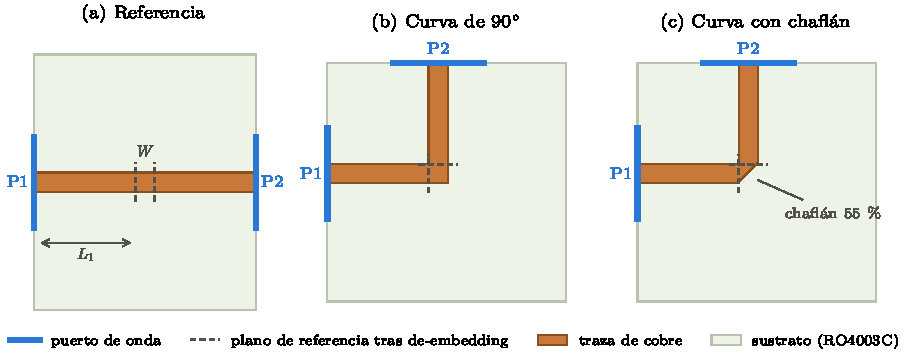
\includegraphics[width=\textwidth]{figuras/fig0_geometria.pdf}
\caption{Vista superior de las estructuras de la curva. Los planos de referencia (líneas punteadas) quedan, tras el de-embedding de $L_1$, en los bordes de la esquina; en la referencia encierran un tramo recto de longitud $W$.}
\label{fig:geo}
\end{figure}

La Figura~\ref{fig:hfss3d} muestra los modelos tal como quedaron construidos en HFSS: la traza de cobre sobre el sustrato, el plano de tierra en la cara inferior, los dos puertos de onda en las caras laterales y la caja de aire que cierra el dominio.

\begin{figure}[htbp]
\centering
\begin{subfigure}[b]{0.325\textwidth}
\centering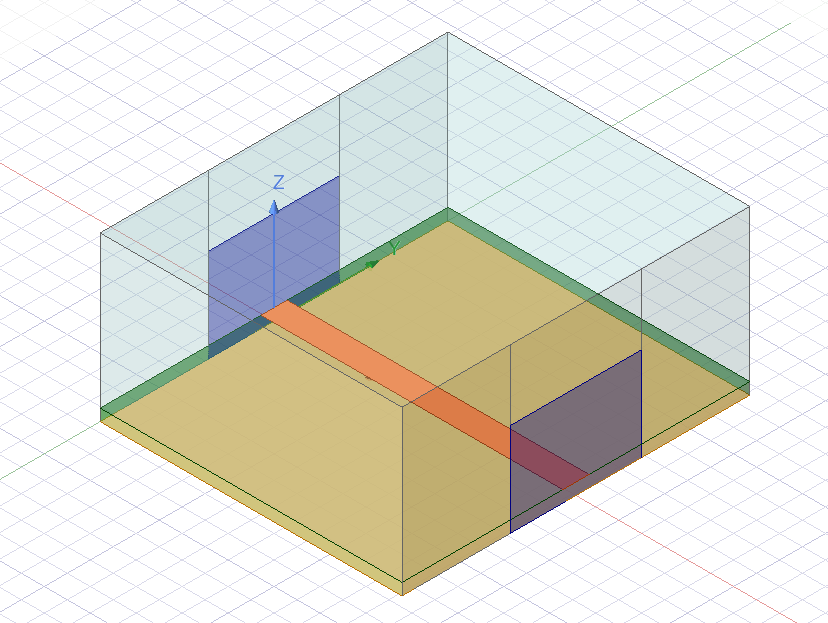
\includegraphics[width=\linewidth]{figuras/hfss3d_referencia.png}
\caption{Referencia}
\end{subfigure}\hfill
\begin{subfigure}[b]{0.325\textwidth}
\centering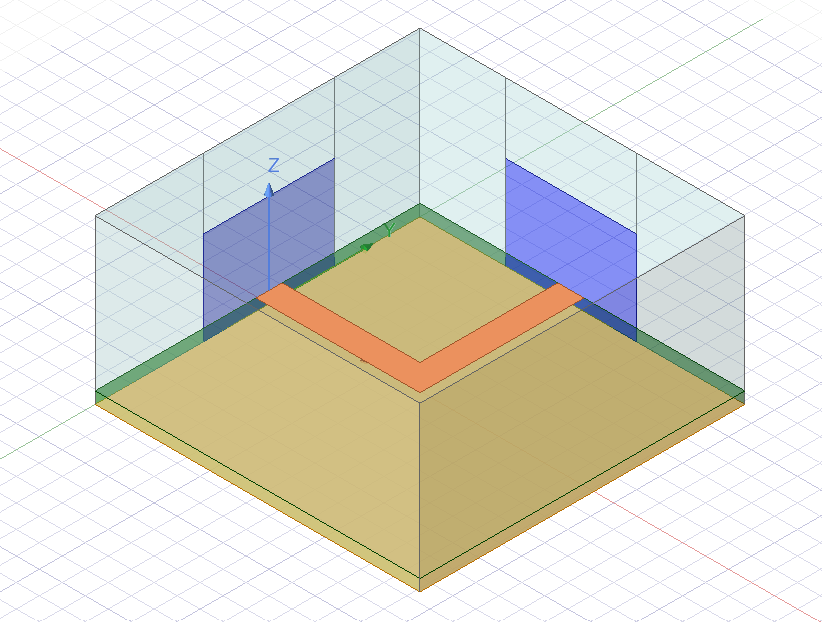
\includegraphics[width=\linewidth]{figuras/hfss3d_curva.png}
\caption{Curva de \ang{90}}
\end{subfigure}\hfill
\begin{subfigure}[b]{0.325\textwidth}
\centering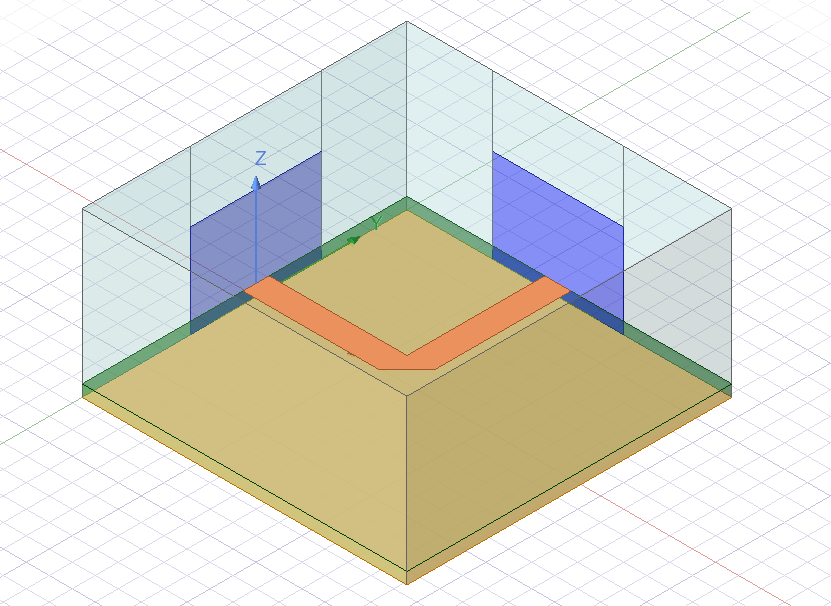
\includegraphics[width=\linewidth]{figuras/hfss3d_chaflan.png}
\caption{Curva con chaflán}
\end{subfigure}
\caption{Modelos 3D de la curva en HFSS. En naranja la traza, en azul los puertos de onda; el bloque inferior es el sustrato con el plano de tierra y el volumen transparente es la caja de aire con frontera de radiación.}
\label{fig:hfss3d}
\end{figure}

\subsection{Resultados}

\subsubsection{Reflexión}
La Figura~\ref{fig:s11} compara $|S_{11}|$ de las tres estructuras y la Tabla~\ref{tab:sparam} resume los valores en frecuencias seleccionadas. La referencia se mantiene por debajo de \SI{<<REFMAX>>}{dB} en toda la banda, lo que valida el montaje. La curva sin compensar crece monotónicamente con la frecuencia, cruza \SI{-30}{dB} a \SI{<<F30>>}{GHz}, \SI{-20}{dB} a \SI{<<F20>>}{GHz} y llega a \SI{<<S11B20>>}{dB} a \SI{20}{GHz}. La curva con chaflán no supera \SI{<<CMAX>>}{dB} en ningún punto, es decir, queda al nivel de la propia referencia.

\begin{figure}[htbp]
\centering
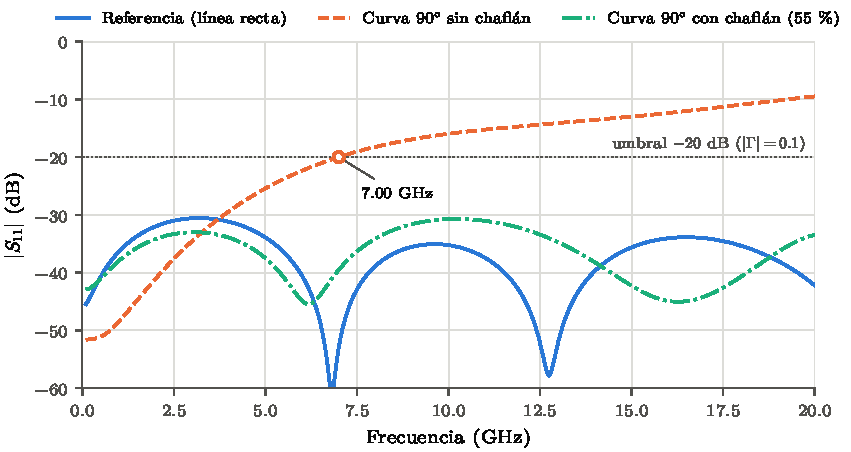
\includegraphics[width=\textwidth]{figuras/fig1_S11_dB.pdf}
\caption{Curva de \ang{90}: magnitud de $S_{11}$. El punto marca la frecuencia a la que la curva sin compensar supera el umbral de $-20$~dB ($|\Gamma|=0.1$, VSWR $=1.22$, 1\,\% de la potencia reflejada).}
\label{fig:s11}
\end{figure}

\begin{figure}[htbp]
\centering
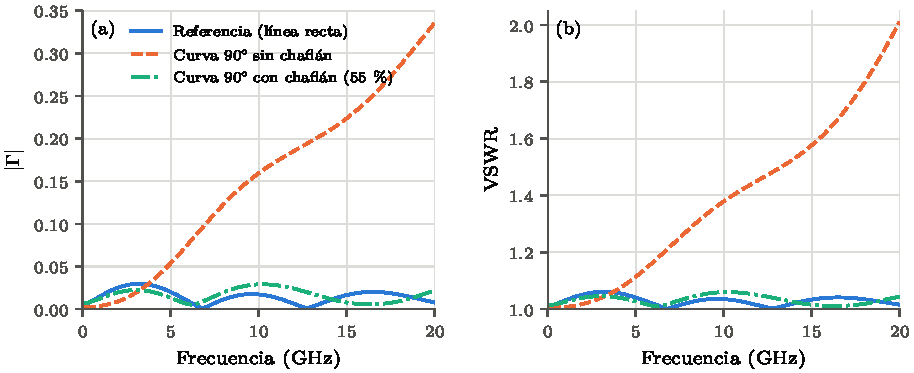
\includegraphics[width=\textwidth]{figuras/fig3_Gamma_VSWR.pdf}
\caption{Curva de \ang{90}: (a) magnitud del coeficiente de reflexión y (b) VSWR.}
\label{fig:gamma}
\end{figure}

La Figura~\ref{fig:gamma} muestra lo mismo en términos de $|\Gamma|$ y VSWR. A \SI{20}{GHz} la curva sin compensar tiene $|\Gamma|=<<GB20>>$ y VSWR $=<<VSWR20B>>$, mientras que la curva con chaflán se mantiene en VSWR $\leq <<VSWRCMAX>>$ en toda la banda.

\begin{table}[htbp]
\centering
\caption{Curva de \ang{90}: parámetros de dispersión en frecuencias seleccionadas.}
\label{tab:sparam}
\small
\setlength{\tabcolsep}{3.2pt}
\begin{tabular}{c cccc cccc cccc}
\toprule
 & \multicolumn{4}{c}{Referencia} & \multicolumn{4}{c}{Curva sin chaflán} & \multicolumn{4}{c}{Curva con chaflán} \\
\cmidrule(lr){2-5}\cmidrule(lr){6-9}\cmidrule(lr){10-13}
$f$ (GHz) & $S_{11}$ & $|\Gamma|$ & VSWR & $S_{21}$ & $S_{11}$ & $|\Gamma|$ & VSWR & $S_{21}$ & $S_{11}$ & $|\Gamma|$ & VSWR & $S_{21}$ \\
 & (dB) & & & (dB) & (dB) & & & (dB) & (dB) & & & (dB) \\
\midrule
<<SROWS>>
\bottomrule
\end{tabular}
\end{table}

\subsubsection{Carácter de la reflexión y circuito equivalente}
En la carta de Smith (Figura~\ref{fig:smith}) la trayectoria de $S_{11}$ de la curva sin compensar arranca cerca del centro, cae a la mitad inferior con un ángulo de \ang{<<ANG5>>} a \SI{5}{GHz} y se aleja del centro al aumentar la frecuencia. Por \eqref{eq:gamma_tau}, un ángulo cercano a \ang{-90} identifica una discontinuidad predominantemente capacitiva. Las simulaciones con y sin pérdidas dan prácticamente la misma $S_{11}$ (diferencia máxima de \SI{<<DS11LOSS>>}{dB} entre 3 y \SI{20}{GHz}), lo que confirma que la reflexión es reactiva: proviene de energía almacenada y no de energía disipada.

\begin{figure}[htbp]
\centering
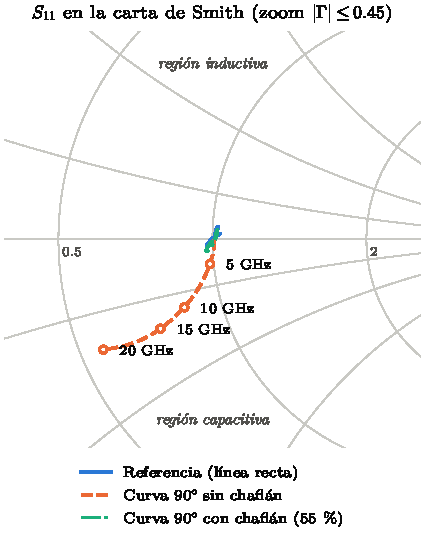
\includegraphics[width=0.5\textwidth]{figuras/fig4_Smith_S11.pdf}
\caption{Curva de \ang{90}: trayectoria de $S_{11}$ en la carta de Smith entre \SI{0.1}{} y \SI{20}{GHz}.}
\label{fig:smith}
\end{figure}

La Figura~\ref{fig:lc} y la Tabla~\ref{tab:lc} muestran los elementos extraídos con \eqref{eq:LC}. Entre 3 y \SI{12}{GHz} los valores son aproximadamente constantes, como corresponde a elementos concentrados. El resultado central es que la capacitancia de la esquina ($C=\SI{<<CB>>}{pF}$) es prácticamente la misma que la de un tramo recto de igual área ($\SI{<<CA>>}{pF}$), mientras que su inductancia por rama ($L=\SI{<<LB>>}{nH}$) es menos de la mitad de la del tramo recto ($\SI{<<LA>>}{nH}$). El chaflán hace lo contrario: reduce la capacitancia a \SI{<<CC>>}{pF} y deja la inductancia casi igual (\SI{<<LC>>}{nH}).

\begin{figure}[htbp]
\centering
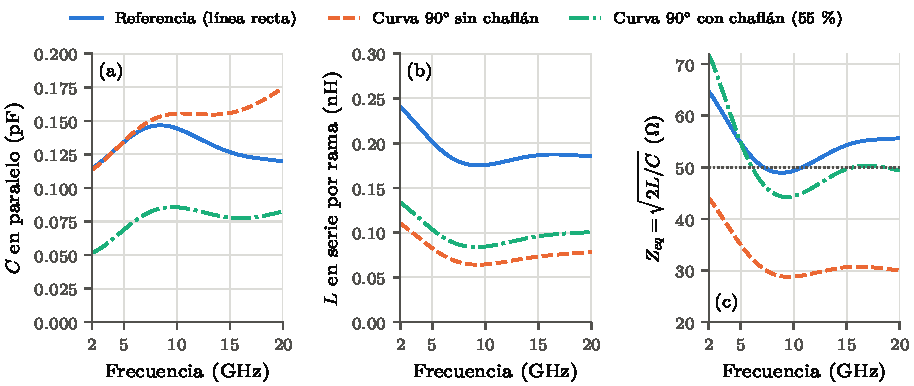
\includegraphics[width=\textwidth]{figuras/fig5_parasitos_LC.pdf}
\caption{Curva de \ang{90}: elementos del circuito equivalente en T extraídos de HFSS: (a) capacitancia en paralelo, (b) inductancia serie por rama y (c) impedancia local equivalente.}
\label{fig:lc}
\end{figure}

\begin{table}[htbp]
\centering
\caption{Curva de \ang{90}: circuito equivalente en T (promedio de 3 a \SI{12}{GHz}).}
\label{tab:lc}
\small
\begin{tabular}{lccccc}
\toprule
Diseño & $C$ (pF) & $L$ por rama (nH) & $Z_{eq}$ ($\Omega$) & $\tau$ (ps) & $|S_{11}|=-20$~dB en \\
\midrule
<<LCROWS>>
\bottomrule
\end{tabular}
\end{table}

\subsubsection{Transmisión y pérdida de inserción}
La Figura~\ref{fig:s21} muestra $|S_{21}|$. La curva sin compensar pierde \SI{<<ILB10>>}{dB} a \SI{10}{GHz} y \SI{<<ILB20>>}{dB} a \SI{20}{GHz}; la curva con chaflán, \SI{<<ILC20>>}{dB} a \SI{20}{GHz}. Para saber de dónde viene esa pérdida se aplicó la separación \eqref{eq:separacion}; el resultado está en la Figura~\ref{fig:rad} y en la Tabla~\ref{tab:potencia}.

\begin{figure}[htbp]
\centering
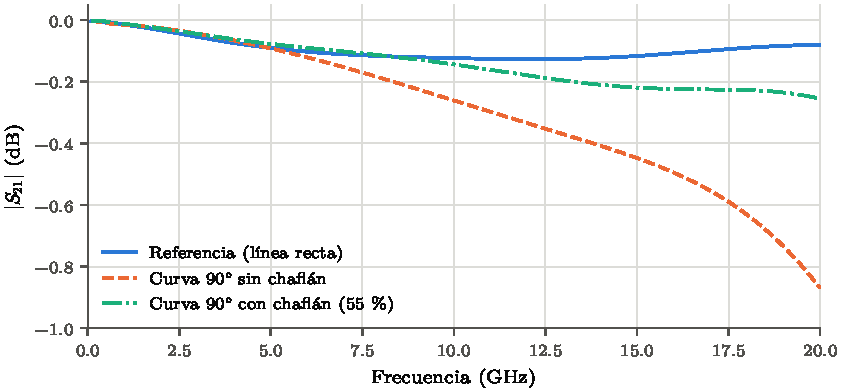
\includegraphics[width=\textwidth]{figuras/fig2_S21_dB.pdf}
\caption{Curva de \ang{90}: magnitud de $S_{21}$ (planos de referencia en los bordes de la esquina).}
\label{fig:s21}
\end{figure}

\begin{figure}[htbp]
\centering
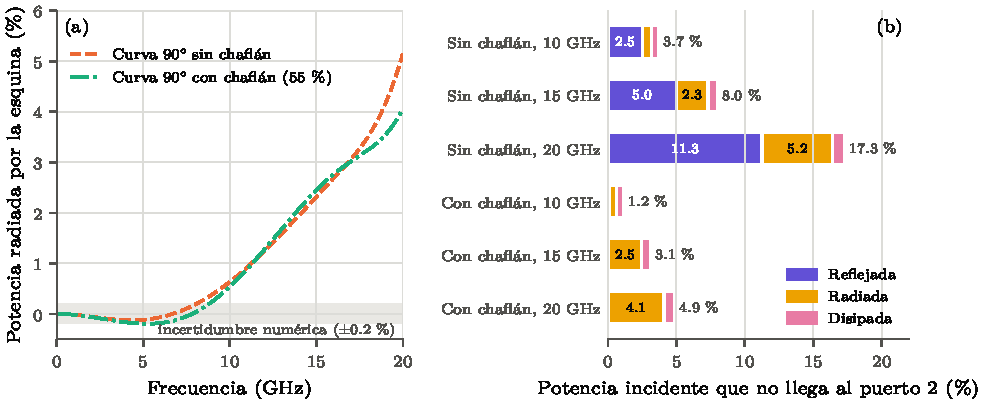
\includegraphics[width=\textwidth]{figuras/fig6_radiacion_potencia.pdf}
\caption{Curva de \ang{90}: (a) potencia radiada por la esquina, obtenida con \eqref{eq:separacion}; la banda gris es la incertidumbre numérica. (b) Destino de la potencia que no llega al puerto 2.}
\label{fig:rad}
\end{figure}

\begin{table}[htbp]
\centering
\caption{Curva de \ang{90}: destino de la potencia incidente (\%). El residuo es el error numérico común a todas las estructuras (pérdida aparente de la referencia sin pérdidas); incertidumbre de la radiada $\pm$<<PISO>>\,\%.}
\label{tab:potencia}
\small
\setlength{\tabcolsep}{4pt}
\begin{tabular}{lcccccccc}
\toprule
Diseño & $f$ (GHz) & Transmitida & Reflejada & Radiada & Disipada & Residuo & IL (dB) & IL$_{\mathrm{refl}}$ (dB) \\
\midrule
<<POWROWS>>
\bottomrule
\end{tabular}
\end{table}

En la curva sin compensar la pérdida de inserción está dominada por la reflexión: a \SI{20}{GHz}, de los \SI{<<ILB20>>}{dB}, \SI{<<ILRB20>>}{dB} se deben solo a la potencia reflejada. La radiación es despreciable por debajo de unos \SI{8}{GHz} y crece rápidamente, aproximadamente como $f^{<<EXPO>>}$ entre 10 y \SI{20}{GHz}. La potencia disipada en cobre y dieléctrico es la misma en las tres estructuras dentro de la incertidumbre, de modo que la esquina no agrega pérdidas óhmicas apreciables.

\subsection{Discusión: explicación física}

\subsubsection{Por qué la esquina refleja}
\label{sec:d1porque}
Para ver qué ocurre dentro de la esquina se exportaron de HFSS los campos $\mathbf{E}$ y $\mathbf{H}$ a \SI{5}{GHz} en dos planos situados a \SI{0.02}{mm} por debajo y por encima de la traza. Con ellos se calcularon la densidad de carga superficial y la densidad de corriente superficial sobre la tira a partir de las condiciones de frontera en un conductor,
\begin{equation}
\rho_s = \varepsilon_0 E_z^{\mathrm{arriba}} - \varepsilon_0\varepsilon_r E_z^{\mathrm{abajo}}, \qquad
\mathbf{J}_s = \hat{\mathbf{z}}\times\left(\mathbf{H}^{\mathrm{arriba}}-\mathbf{H}^{\mathrm{abajo}}\right),
\label{eq:saltos}
\end{equation}
y se representaron en la Figura~\ref{fig:carga}. Se eligió \SI{5}{GHz}, por debajo del umbral de \SI{7}{GHz}, para observar la distribución que da origen a la reflexión.

\begin{figure}[htbp]
\centering
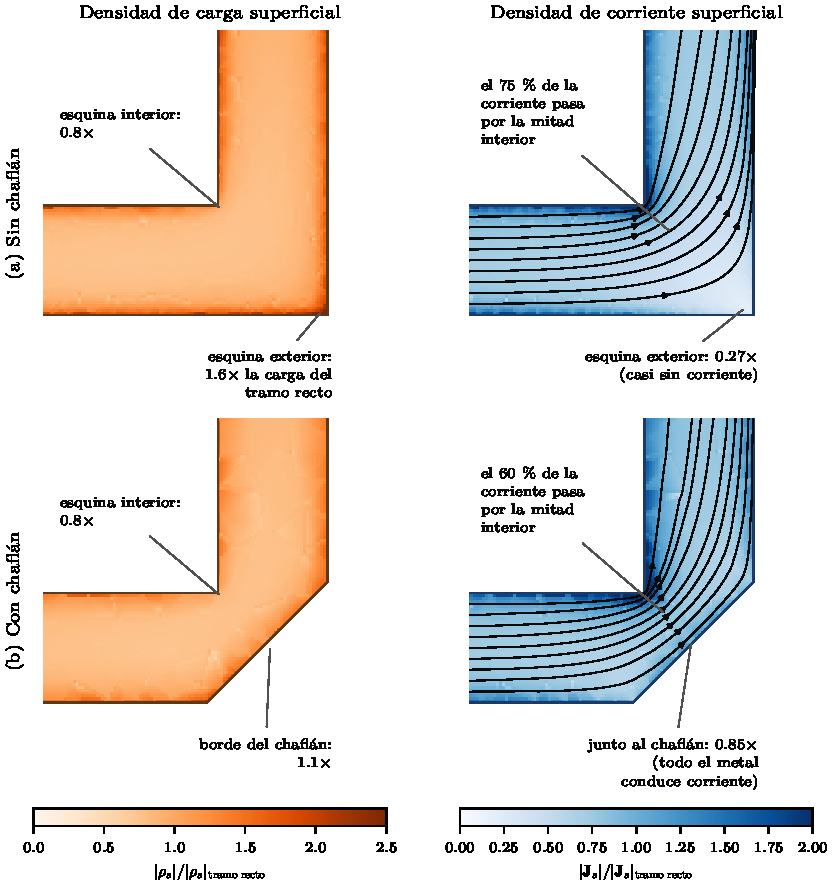
\includegraphics[width=\textwidth]{figuras/fig7_carga_corriente.pdf}
\caption{Curva de \ang{90}: densidad de carga superficial $|\rho_s|$ (izquierda) y densidad de corriente superficial $|\mathbf{J}_s|$ con sus líneas de flujo (derecha), calculadas con \eqref{eq:saltos} a partir de los campos de HFSS a \SI{5}{GHz}, para (a) la curva sin chaflán y (b) la curva con chaflán. Ambas están normalizadas a su promedio en una sección del brazo situada a $2.5W$ de la esquina; los factores indicados son promedios en un cuadrado de lado $W/4$ en cada esquina, o en una franja de ancho $W/4$ a lo largo del chaflán.}
\label{fig:carga}
\end{figure}

A lo ancho de la tira, tanto la carga como la corriente se concentran en los bordes, como corresponde a una línea a alta frecuencia. En la esquina, sin embargo, ambas se separan. En la curva sin chaflán (Figura~\ref{fig:carga}a) la esquina exterior tiene <<HCEXT>> veces la carga del tramo recto, pero solo <<HJEXT>> veces su corriente. Visto de otra forma, la mitad exterior del cuadrado de la esquina guarda el <<HQOUT>>\,\% de su carga, mientras que el <<HIIN>>\,\% de la corriente que atraviesa la esquina pasa por la mitad interior de su diagonal; en un tramo recto ambos repartos serían de 50\,\%. La corriente toma el camino corto por la esquina interior, y la esquina exterior almacena carga, y por lo tanto energía eléctrica, casi sin corriente que la acompañe, y por lo tanto casi sin energía magnética.

En la curva con chaflán (Figura~\ref{fig:carga}b) ese metal ya no existe. La carga a lo largo del borde del chaflán es <<HCCH>> veces la del tramo recto y la corriente junto a él <<HJCH>> veces: todo el metal que queda conduce corriente, y la corriente se reparte de forma más pareja, con el <<HIINC>>\,\% por la mitad interior.

\paragraph{Consistencia con la extracción del circuito.} Sumando la carga dentro del cuadrado de la esquina se obtiene <<HQB>> veces la de un tramo recto de igual área, en acuerdo con el cociente de capacitancias extraído de los parámetros $S$ (<<RCB>>, Tabla~\ref{tab:lc}). Para la curva con chaflán ambos valores muestran la misma reducción fuerte (<<HQC>> y <<RCC>>). La coincidencia es menor porque la capacitancia de la red en T es un parámetro equivalente que reproduce los parámetros $S$ en los planos de referencia, y no exactamente la carga contenida en el cuadrado; la diferencia crece cuando la forma del metal se aleja de la de un tramo de línea, como con el chaflán, que deja solo el \SI{40}{\percent} del área del cuadrado.

En términos de \eqref{eq:poynting}, la región de la esquina almacena aproximadamente la misma energía eléctrica que un tramo recto de igual área, pero mucha menos energía magnética, porque la corriente recorre un camino más corto. El resultado es un exceso neto de energía eléctrica, es decir, un comportamiento capacitivo, que es exactamente lo que muestran la carta de Smith y la extracción de HFSS: $C$ igual a la del tramo recto y $L$ menor a la mitad.

Visto como línea de transmisión, el desequilibrio entre $L$ y $C$ equivale a insertar en la línea de \SI{50}{\ohm} un tramo corto de $Z_{eq}\approx\SI{<<ZEQB>>}{\ohm}$. Esa es la desadaptación de impedancias que produce la reflexión. El chaflán elimina justamente el metal de la esquina exterior, el que almacenaba carga sin conducir corriente; por eso reduce $C$ casi a la mitad sin cambiar mucho $L$, y restituye $Z_{eq}\approx\SI{<<ZEQC>>}{\ohm}$.

\subsubsection{A partir de qué frecuencia el efecto es significativo}
Se tomó como criterio de efecto significativo $|S_{11}|>-20$~dB, es decir, $|\Gamma|>0.1$, VSWR $>1.22$ o más del 1\,\% de la potencia reflejada. Con este criterio se distinguen tres regiones para la curva sin compensar:
\begin{itemize}
\item \textbf{Por debajo de unos \SI{4}{GHz}} la curva es indistinguible de la línea recta: su $|S_{11}|$ queda por debajo de \SI{-30}{dB}, al nivel de la referencia.
\item \textbf{Entre unos 4 y \SI{7}{GHz}} el efecto es medible pero pequeño.
\item \textbf{A partir de \SI{<<F20>>}{GHz}} el efecto es significativo, y por encima de unos \SI{12}{GHz} se suma una radiación mayor al 1\,\%.
\end{itemize}

La explicación electromagnética está en \eqref{eq:poynting}. Mientras la esquina sea pequeña frente a $\lambda_g$, la distribución de campo en su vecindad es cuasiestática, y la diferencia de energías $W_m-W_e$ por unidad de $|I|^2$ es prácticamente independiente de la frecuencia. La reactancia neta, en cambio, lleva el factor $\omega$, y por eso crece linealmente con la frecuencia hasta que deja de ser despreciable frente a $Z_0$. Con el valor extraído $\tau=\SI{<<TAUB>>}{ps}$, la ecuación \eqref{eq:gamma_tau} predice $|\Gamma|=0.1$ a
\[
f = \frac{0.1}{\pi\tau} = \SI{<<FPRED>>}{GHz},
\]
en buen acuerdo con los \SI{<<F20>>}{GHz} que da la simulación de onda completa.

\begin{figure}[htbp]
\centering
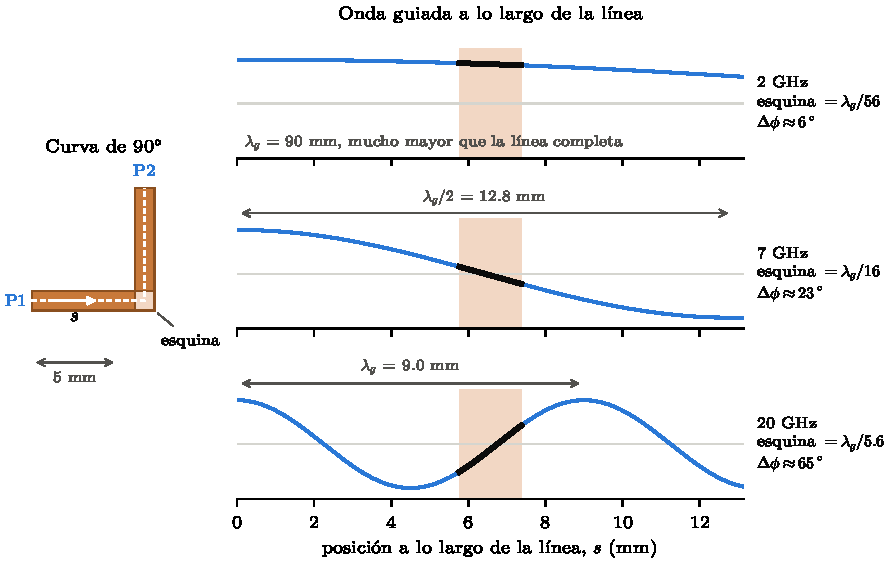
\includegraphics[width=\textwidth]{figuras/fig8_escala_lambda.pdf}
\caption{Tamaño de la esquina frente a la longitud de onda guiada. A la izquierda, la curva y la coordenada $s$ a lo largo del eje de la línea. A la derecha, una instantánea de la onda guiada, $\cos(2\pi s/\lambda_g)$, a 2, 7 y \SI{20}{GHz} en función de $s$. La franja marca la zona de la esquina (su diagonal, $W\sqrt{2}=\SI{1.61}{mm}$), el tramo negro es la parte de la onda que cae dentro de ella y $\Delta\phi$ es el desfase de la onda a través de la esquina.}
\label{fig:escala}
\end{figure}

La Figura~\ref{fig:escala} compara la esquina con la longitud de onda guiada $\lambda_g$. A \SI{2}{GHz} ($\lambda_g=\SI{<<LG2>>}{mm}$) la onda apenas cambia a lo largo de toda la estructura y la esquina mide $\lambda_g/<<FRAC2>>$: todos los puntos de la esquina ven prácticamente el mismo voltaje y la misma corriente al mismo tiempo. A \SI{<<F20>>}{GHz}, donde el efecto se vuelve significativo, la esquina mide todavía $\lambda_g/<<FRAC7>>$ y la fase cambia solo \ang{<<FASE7>>} a través de ella: la esquina sigue siendo eléctricamente pequeña y el modelo concentrado es válido. Esto muestra que el efecto no aparece porque la esquina sea ``grande'', sino porque el desequilibrio de energías multiplicado por $\omega$ deja de ser despreciable. A \SI{20}{GHz} ($\lambda_g=\SI{<<LG20>>}{mm}$) la esquina mide $\lambda_g/<<FRAC20>>$ y la fase cambia \ang{<<FASE20>>} a través de ella. Ahí ya no puede tratarse como un punto: el modelo concentrado empieza a perder validez (la $C$ extraída deja de ser constante en la Figura~\ref{fig:lc}a) y la radiación crece rápidamente.

\subsubsection{Por qué el chaflán elimina la reflexión pero no la radiación}
\label{sec:d1rad}
Por el método de imágenes, la corriente $I$ de la tira y la corriente de retorno en el plano de tierra equivalen a dos corrientes opuestas, $I$ y $-I$, separadas $2h$ (Figura~\ref{fig:imagen}a). Lejos de la línea sus campos casi se anulan: el campo del par decae como $2h/r^2$ en lugar de $1/r$ (Figura~\ref{fig:imagen}b). Además, a lo largo de un tramo recto la onda viaja con $\beta=k_0\sqrt{\varepsilon_{\mathrm{eff}}}>k_0$, de modo que las contribuciones de los distintos elementos de corriente interfieren destructivamente en el espacio libre. Por ambas razones la línea recta guía la energía sin radiar.

\begin{figure}[htbp]
\centering
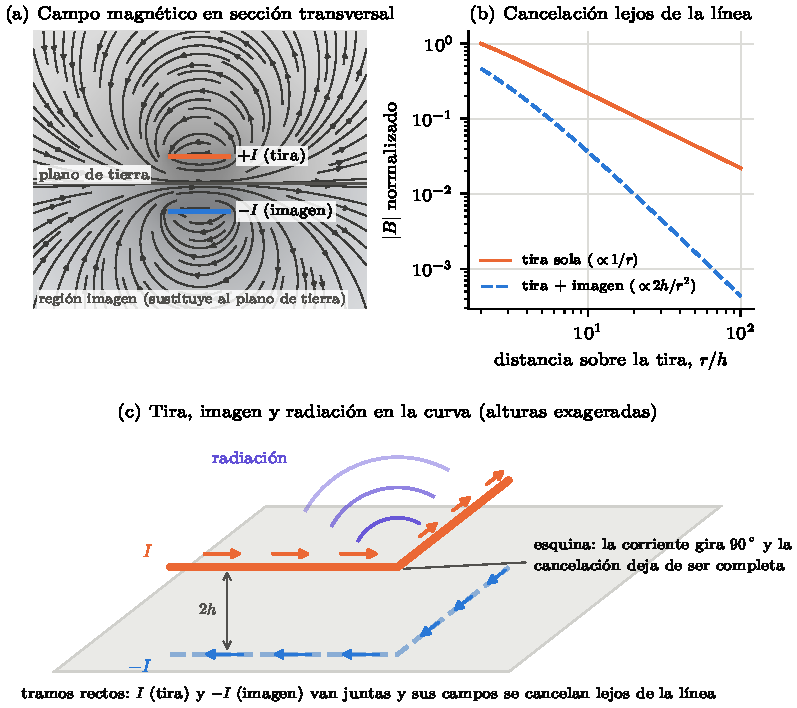
\includegraphics[width=\textwidth]{figuras/fig9_imagen_radiacion.pdf}
\caption{(a) Líneas de campo magnético de la tira y su imagen en sección transversal (el semiplano inferior es la región imagen que sustituye al plano de tierra). (b) Decaimiento del campo con la distancia para la tira sola y para el par tira--imagen. (c) Esquema de la curva: a lo largo de los tramos rectos $I$ y $-I$ viajan juntas; en la esquina la corriente gira \ang{90} y la cancelación deja de ser completa.}
\label{fig:imagen}
\end{figure}

En la esquina la corriente cambia de dirección bruscamente (Figura~\ref{fig:imagen}c). Las contribuciones de los dos brazos ya no apuntan en la misma dirección y no se compensan entre sí, de modo que la esquina radia como una pequeña antena \cite{lewin}. El chaflán corrige el exceso de carga, que es la causa de la reflexión, pero la corriente sigue girando \ang{90}; por eso ambas curvas radian cantidades similares (\SI{<<RADB20>>}{\percent} y \SI{<<RADC20>>}{\percent} a \SI{20}{GHz}). La radiación crece con la frecuencia y con el espesor eléctrico del sustrato, porque la separación $2h$ entre la tira y su imagen deja de ser despreciable frente a $\lambda_0$. En sustratos más gruesos o a frecuencias mayores sería el efecto dominante.

%======================================================================
\section{Discontinuidad 2: cambio abrupto de ancho}
\label{sec:d2}

\subsection{Diseño y estructuras simuladas}
Se unió de golpe la línea de \SI{50}{\ohm} ($W_1=\SI{1.14}{mm}$) con una línea de \SI{100}{\ohm} ($W_2=\SI{0.29}{mm}$) del mismo sustrato y el mismo cobre, como si se empalmaran dos pistas de distinto grosor. La línea de \SI{100}{\ohm} se eligió porque da una desadaptación grande y fácil de interpretar: por \eqref{eq:gamma0}, con las impedancias de \eqref{eq:z0}, $\Gamma_0=<<D2_G0Q>>$, VSWR $=<<D2_VSWR0Q>>$ y un <<D2_PREF0Q>>\,\% de la potencia reflejada. Por unidad de longitud, la línea angosta tiene $C'=\SI{<<D2_CP2>>}{pF/m}$ y $L'=\SI{<<D2_LP2>>}{nH/m}$, frente a $C'=\SI{<<D2_CP1>>}{pF/m}$ y $L'=\SI{<<D2_LP1>>}{nH/m}$ de la ancha: <<D2_RCP>> veces la capacitancia y <<D2_RLP>> veces la inductancia. La relación de anchos es $W_1/W_2=<<D2_RGUP>>$.

Se simularon seis estructuras (Figura~\ref{fig:dgeo}):
\begin{itemize}
\item \textbf{Escalón abrupto:} tramos de $L_1=\SI{6}{mm}$ de cada línea unidos en un plano. Tras el de-embedding ambos planos de referencia coinciden con el escalón.
\item \textbf{Transición gradual:} el mismo cambio repartido en $L_t=\SI{10}{mm}$ con el perfil exponencial de \eqref{eq:taper}. Cumple el papel que tuvo el chaflán en la curva: permite separar el efecto de la diferencia de impedancias del efecto de que el cambio sea brusco. Por \eqref{eq:taper}, su primer nulo de reflexión debería estar en \SI{<<D2_FNULL>>}{GHz}, donde $L_t=\lambda_g/2$ con la permitividad efectiva promedio de ambas líneas ($<<D2_EEM>>$).
\item \textbf{Referencias:} una línea recta de \SI{50}{\ohm} y una de \SI{100}{\ohm}, de longitud $2L_1$ y de-embebidas hasta longitud cero. Validan cada línea y miden el error numérico de los puertos (Sección~\ref{sec:correccion}).
\end{itemize}
Como en la curva, de cada estructura se simuló un gemelo sin pérdidas. La Figura~\ref{fig:dhfss} muestra los modelos en HFSS.

\begin{figure}[htbp]
\centering
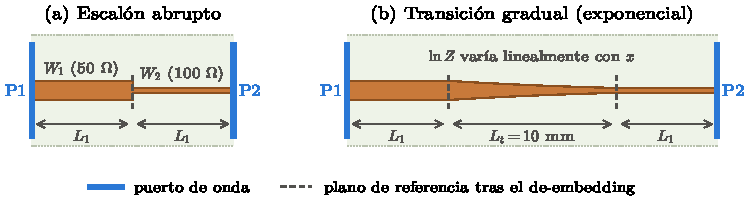
\includegraphics[width=\textwidth]{figuras/fig_d2_geometria.pdf}
\caption{Vista superior del escalón y de la transición gradual (el sustrato se muestra recortado; mide \SI{15.1}{mm} de ancho). Los planos de referencia quedan, tras el de-embedding de $L_1$, en el escalón o en los extremos de la transición.}
\label{fig:dgeo}
\end{figure}

\begin{figure}[htbp]
\centering
\begin{subfigure}[b]{0.49\textwidth}
\centering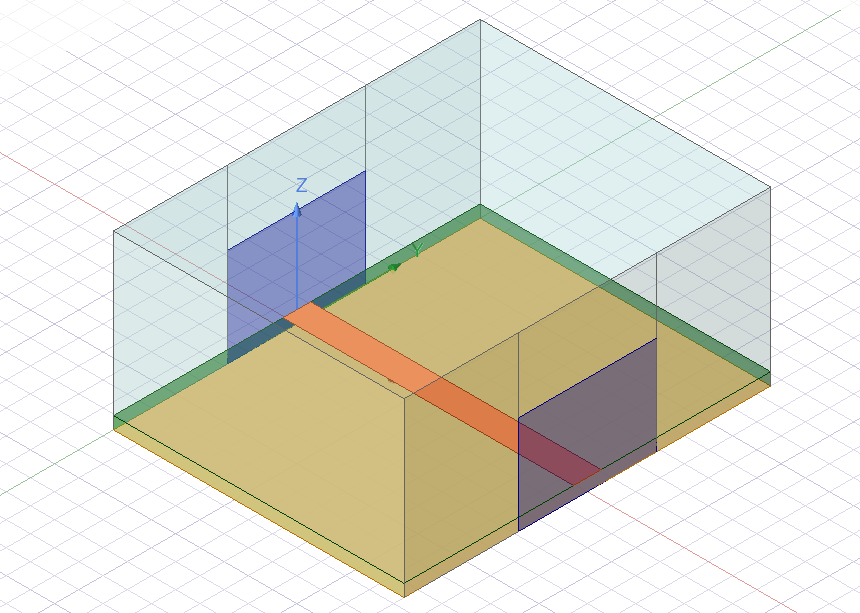
\includegraphics[width=0.9\linewidth]{figuras/hfss3d_d2_ref50.png}
\caption{Referencia de \SI{50}{\ohm}}
\end{subfigure}\hfill
\begin{subfigure}[b]{0.49\textwidth}
\centering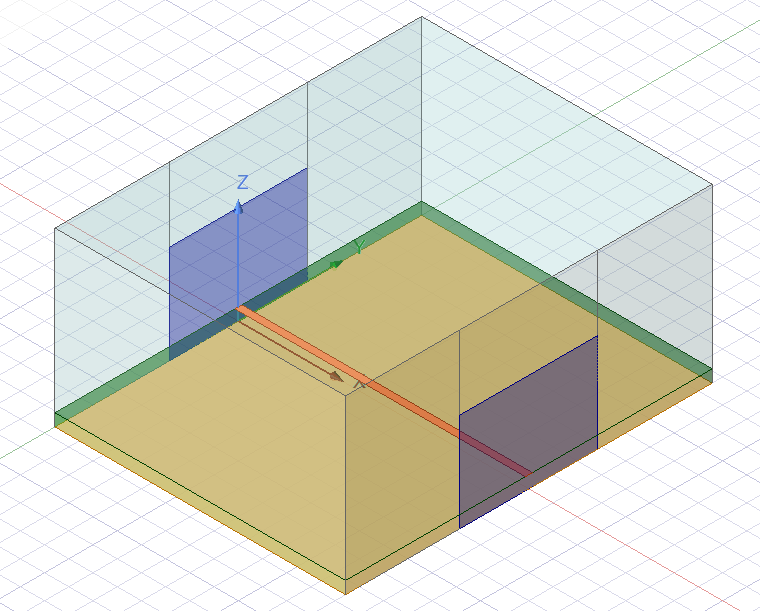
\includegraphics[width=0.9\linewidth]{figuras/hfss3d_d2_ref100.png}
\caption{Referencia de \SI{100}{\ohm}}
\end{subfigure}\\[6pt]
\begin{subfigure}[b]{0.49\textwidth}
\centering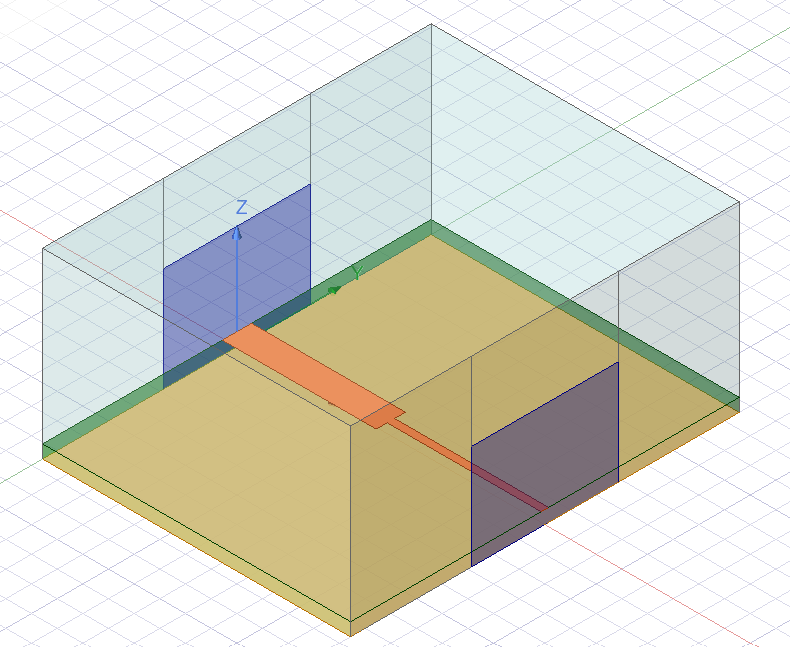
\includegraphics[width=0.9\linewidth]{figuras/hfss3d_d2_escalon.png}
\caption{Escalón abrupto}
\end{subfigure}\hfill
\begin{subfigure}[b]{0.49\textwidth}
\centering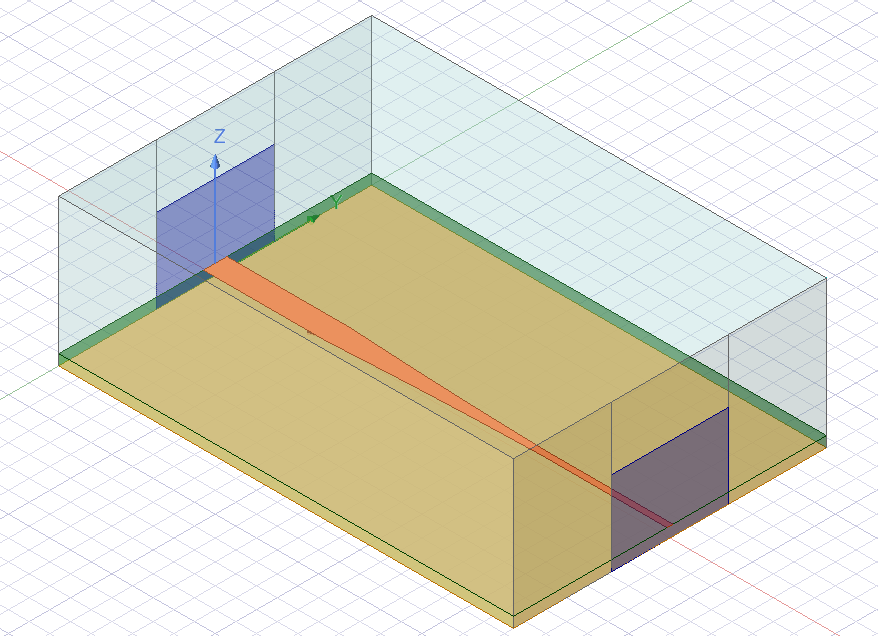
\includegraphics[width=0.9\linewidth]{figuras/hfss3d_d2_transicion.png}
\caption{Transición gradual}
\end{subfigure}
\caption{Modelos 3D del cambio de ancho en HFSS, con la misma caja de aire y los mismos puertos que la curva.}
\label{fig:dhfss}
\end{figure}

\subsection{Tratamiento numérico propio de esta discontinuidad}

\paragraph{Validación de las líneas.} Con los puertos sin renormalizar, HFSS reporta la impedancia característica y la constante de propagación $\gamma=\alpha+j\beta$ de cada línea, de donde $\varepsilon_{\mathrm{eff}}=(\beta/k_0)^2$. La Tabla~\ref{tab:dlineas} las compara con las fórmulas cuasi-estáticas. A \SI{1}{GHz} la impedancia difiere en \SI{<<D2_DZ50>>}{\percent} y \SI{<<D2_DZ100>>}{\percent} y la permitividad efectiva en \SI{<<D2_DE50>>}{\percent} y \SI{<<D2_DE100>>}{\percent}, dentro de la precisión de \eqref{eq:eeff} y \eqref{eq:z0}. Al subir la frecuencia $\varepsilon_{\mathrm{eff}}$ crece por dispersión, más en la línea ancha, que concentra más campo en el sustrato.

\begin{table}[htbp]
\centering
\caption{Líneas de la discontinuidad 2: fórmulas cuasi-estáticas \eqref{eq:eeff}--\eqref{eq:z0} frente a los puertos de HFSS (referencias sin pérdidas).}
\label{tab:dlineas}
\small
\setlength{\tabcolsep}{4.5pt}
\begin{tabular}{lccccccc}
\toprule
 & \multicolumn{2}{c}{Fórmulas} & \multicolumn{2}{c}{$Z_0$ HFSS ($\Omega$)} & \multicolumn{3}{c}{$\varepsilon_{\mathrm{eff}}$ HFSS} \\
\cmidrule(lr){2-3}\cmidrule(lr){4-5}\cmidrule(lr){6-8}
Línea & $Z_0$ ($\Omega$) & $\varepsilon_{\mathrm{eff}}$ & \SI{1}{GHz} & \SI{20}{GHz} & \SI{1}{GHz} & \SI{10}{GHz} & \SI{20}{GHz} \\
\midrule
<<D2_LINROWS>>
\bottomrule
\end{tabular}
\end{table}

\paragraph{Corrección del error de puerto.}
\label{sec:correccion}
Las líneas de referencia, de-embebidas hasta longitud cero, deberían dar $S_{11}=0$ y $S_{21}=1$. En la simulación muestran $|S_{11}|$ de hasta \SI{<<D2_FLOOR50>>}{dB} con una ondulación periódica (Figura~\ref{fig:dcorr}a), el mismo residuo que se observó en la referencia de la curva. Su forma corresponde a un pequeño desacople $g$ entre el modo del puerto, que HFSS calcula en 2D, y la línea en la malla 3D. Ese desacople aparece en ambos extremos con signo opuesto, separado una distancia $2L_1$:
\begin{equation}
S_{11}^{\mathrm{ref}} \approx g\left(e^{2j\beta L_1}-e^{-2j\beta L_1}\right).
\label{eq:gpuerto}
\end{equation}
Se ajustó $g(f)$ como un polinomio complejo de grado 3 por mínimos cuadrados ($|g|\leq <<D2_GP50>>$ en la línea de \SI{50}{\ohm} y $\leq <<D2_GP100>>$ en la de \SI{100}{\ohm}). Con $g$ y la transmisión de cada referencia se armó una caja de error por puerto y se quitó de las mediciones en cascada inversa, con matrices de transferencia:
\begin{equation}
\mathbf{T}_{\text{escalón}} = \mathbf{T}_{A}^{-1}\,\mathbf{T}_{\text{medida}}\,\mathbf{T}_{B}^{-1},
\label{eq:deembed}
\end{equation}
donde $A$ es la caja del puerto 1 (línea de \SI{50}{\ohm}) y $B$ la del puerto 2 (línea de \SI{100}{\ohm}). Los diseños con pérdidas se corrigieron con las referencias con pérdidas, y los sin pérdidas con las sin pérdidas. La corrección se puede comprobar de forma independiente: en una red sin pérdidas y recíproca debe cumplirse $|S_{11}|=|S_{22}|$. En el escalón sin pérdidas, la diferencia máxima entre ambos baja de <<D2_ASIMB0_RAW>> a <<D2_ASIMB0_COR>> (Figura~\ref{fig:dcorr}b). Todos los resultados de esta sección están corregidos.

\begin{figure}[htbp]
\centering
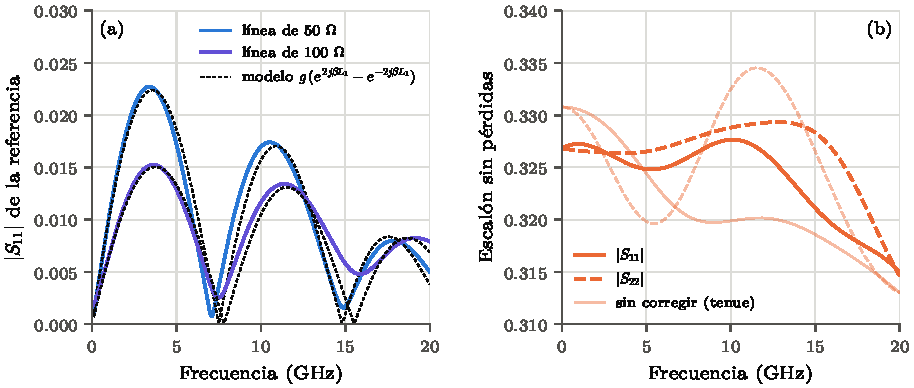
\includegraphics[width=\textwidth]{figuras/fig_d2_correccion.pdf}
\caption{(a) $|S_{11}|$ de las líneas de referencia sin pérdidas y el modelo \eqref{eq:gpuerto} ajustado. (b) $|S_{11}|$ y $|S_{22}|$ del escalón sin pérdidas antes (tenue) y después de quitar las cajas de error; sin pérdidas ambas deben coincidir.}
\label{fig:dcorr}
\end{figure}

\paragraph{Extracción del circuito equivalente.}
\label{sec:ajuste}
El método de la curva no sirve aquí: la unión es casi una conexión directa y su $C$ es tan pequeña que $Z_{21}$ es enorme, de modo que \eqref{eq:LC} amplifica cualquier error. En su lugar se ajustó el circuito de la Figura~\ref{fig:circescalon} a los parámetros $S$ corregidos por mínimos cuadrados, entre 1 y \SI{20}{GHz}, sobre $S_{11}$, $S_{22}$ y $S_{21}$ complejos a la vez. Se ajustaron tres parámetros: $C$, $L_s$ y un factor $k$ que multiplica la impedancia de referencia del puerto 2. A primer orden en $\omega$ los datos solo fijan $L_s$ y $C$ (ecuación \eqref{eq:zent}), así que el reparto se tomó como en \cite{gupta}, $L_1/L_s=<<D2_ALFA>>$. El factor $k$ absorbe una diferencia independiente de la frecuencia entre el cociente de impedancias que reportan los puertos y el que ``ve'' el escalón, porque en una línea que no es TEM pura la impedancia depende de cómo se defina (potencia y corriente, potencia y voltaje, o voltaje y corriente); con él, ningún error en $Z_2$ se confunde con una capacitancia o una inductancia.

\subsection{Resultados}

\subsubsection{Reflexión}
La Figura~\ref{fig:dsdb}a muestra la reflexión del escalón vista desde ambos lados y la de la transición gradual, y la Tabla~\ref{tab:dsparam} resume los valores. El escalón refleja $|\Gamma|=<<D2_GB01>>$ ($|S_{11}|=\SI{<<D2_S11B01>>}{dB}$) ya a \SI{0.1}{GHz}, exactamente lo que predice \eqref{eq:gamma0}, y en toda la banda se mantiene entre <<D2_GBMIN>> y <<D2_GBMAX>> (VSWR entre <<D2_VBMIN>> y <<D2_VBMAX>>, Figura~\ref{fig:dgamma}). $|S_{11}|$ y $|S_{22}|$ coinciden: la reflexión es la misma desde ambos lados, como debe ocurrir en una unión sin pérdidas. La ligera disminución hacia \SI{20}{GHz} sigue a la dispersión de las líneas: la impedancia de la línea angosta en HFSS baja de \SI{<<D2_Z2H1>>}{\ohm} a \SI{<<D2_Z2H20>>}{\ohm}, y el $\Gamma_0$ calculado con las impedancias de los puertos baja de <<D2_G0H>> a <<D2_G0H20>>.

\begin{figure}[htbp]
\centering
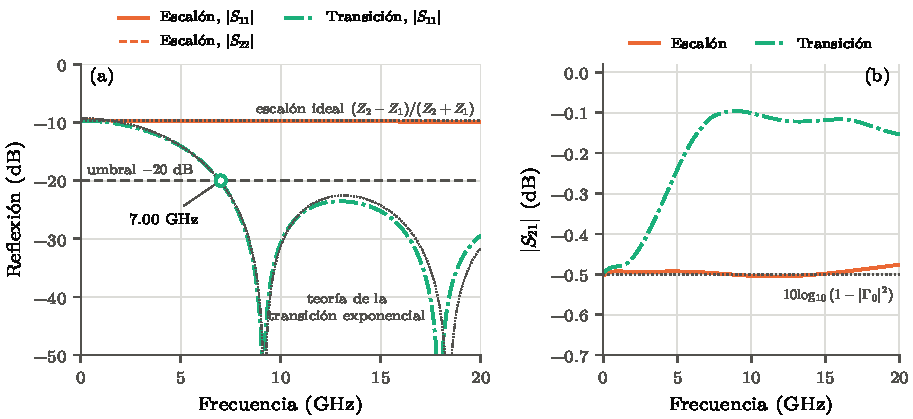
\includegraphics[width=\textwidth]{figuras/fig_d2_S_dB.pdf}
\caption{Cambio de ancho: (a) reflexión del escalón vista desde la línea de \SI{50}{\ohm} ($S_{11}$) y desde la de \SI{100}{\ohm} ($S_{22}$), y de la transición gradual; las líneas punteadas son \eqref{eq:gamma0} y \eqref{eq:taper}. (b) Transmisión; la línea punteada es el límite que impone la reflexión del escalón ideal.}
\label{fig:dsdb}
\end{figure}

La transición gradual parte del mismo valor (<<D2_GC01>> a \SI{0.1}{GHz}), cae por debajo de $-20$~dB a \SI{<<D2_FT20>>}{GHz} y tiene nulos en \SI{<<D2_FTN1>>}{} y \SI{<<D2_FTN2>>}{GHz}, frente a \SI{<<D2_FNULL>>}{} y \SI{<<D2_FNULL2>>}{GHz} que predice \eqref{eq:taper}. Por encima de \SI{10}{GHz} su reflexión no supera $|\Gamma|=<<D2_GCMAXHI>>$ (\SI{<<D2_S11CMAXHI>>}{dB}, VSWR $<<D2_VCMAXHI>>$). La teoría de \eqref{eq:taper}, que no tiene ningún parámetro ajustado, reproduce la curva de HFSS en toda la banda.

\begin{figure}[htbp]
\centering
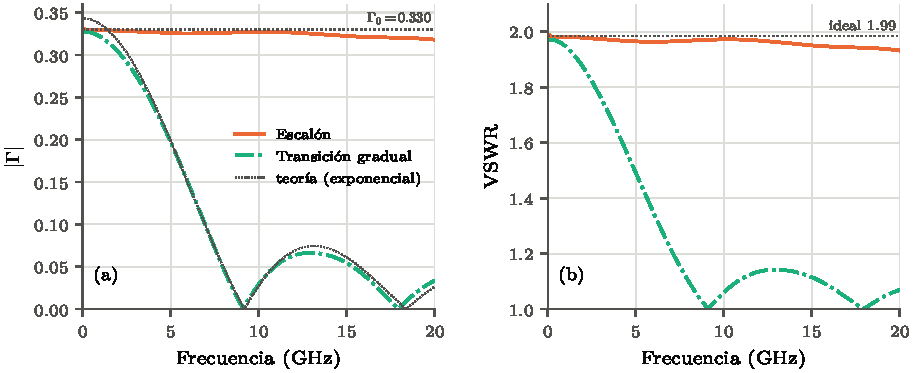
\includegraphics[width=\textwidth]{figuras/fig_d2_Gamma_VSWR.pdf}
\caption{Cambio de ancho: (a) magnitud del coeficiente de reflexión vista desde la línea de \SI{50}{\ohm} y (b) VSWR. La línea punteada horizontal es el escalón ideal \eqref{eq:gamma0}.}
\label{fig:dgamma}
\end{figure}

\begin{table}[htbp]
\centering
\caption{Cambio de ancho: parámetros de dispersión en frecuencias seleccionadas, vistos desde la línea de \SI{50}{\ohm}.}
\label{tab:dsparam}
\small
\setlength{\tabcolsep}{3.6pt}
\begin{tabular}{c ccccc cccc}
\toprule
 & \multicolumn{5}{c}{Escalón abrupto} & \multicolumn{4}{c}{Transición gradual} \\
\cmidrule(lr){2-6}\cmidrule(lr){7-10}
$f$ (GHz) & $S_{11}$ (dB) & $|\Gamma|$ & VSWR & $\angle S_{11}$ (°) & $S_{21}$ (dB) & $S_{11}$ (dB) & $|\Gamma|$ & VSWR & $S_{21}$ (dB) \\
\midrule
<<D2_SROWS2>>
\bottomrule
\end{tabular}
\end{table}

\subsubsection{Carácter de la reflexión y circuito equivalente}
En la carta de Smith (Figura~\ref{fig:dsmith}) el escalón no traza una curva sino dos pequeños arcos casi puntuales: $S_{11}$ cerca de $+<<D2_GB01>>$ (la línea de \SI{50}{\ohm} ve una carga de unos \SI{100}{\ohm}) y $S_{22}$ cerca de $-<<D2_GB01>>$ (la de \SI{100}{\ohm} ve unos \SI{50}{\ohm}). La transición, en cambio, describe una espiral hacia el centro: la reflexión se reduce y su fase gira con el retardo de ida y vuelta a lo largo de la transición. Las versiones con y sin pérdidas del escalón dan $|S_{11}|$ iguales dentro de <<D2_DS11LOSS2>>.

\begin{figure}[htbp]
\centering
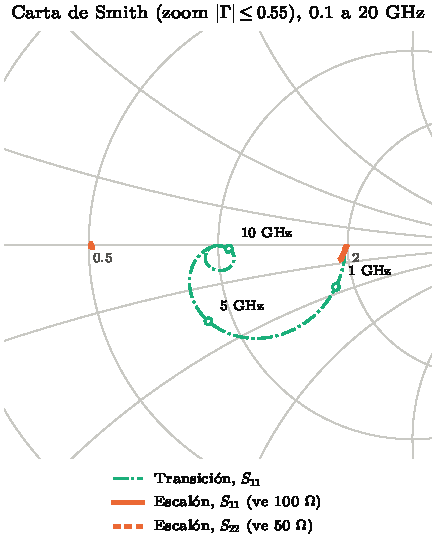
\includegraphics[width=0.5\textwidth]{figuras/fig_d2_Smith.pdf}
\caption{Cambio de ancho: trayectorias en la carta de Smith entre \SI{0.1}{} y \SI{20}{GHz}.}
\label{fig:dsmith}
\end{figure}

La parte reactiva se ve mejor en la fase (Figura~\ref{fig:dfase}a). Desde la línea de \SI{50}{\ohm}, la fase de $S_{11}$ se aleja de \ang{0} linealmente con la frecuencia y llega a \ang{<<D2_ANGB20>>} a \SI{20}{GHz}; desde la de \SI{100}{\ohm} la fase de $-S_{22}$ no se aparta más de \ang{<<D2_ANG22MAX>>}. La reactancia que se ve en el plano del escalón (Figura~\ref{fig:dfase}b) es proporcional a $\omega$, como corresponde a elementos concentrados. El ajuste del circuito (Tabla~\ref{tab:dfit}) da $C=(<<D2_CEXC>>\pm<<D2_ECEXC>>)$~fF y $L_s=(<<D2_LEXC>>\pm<<D2_ELEXC>>)$~pH, donde la incertidumbre es la dispersión entre el diseño con y sin pérdidas y entre rangos de ajuste. Con la corrección de puertos el residuo del ajuste es de <<D2_RMSFIT>>; sin ella es cuatro veces mayor (<<D2_RMSRAW>>) y la capacitancia se duplica artificialmente (\SI{<<D2_CRAW>>}{fF}). Las fórmulas de Gupta et al.\ \eqref{eq:gupta}, extrapoladas ligeramente fuera de su rango ($W_1/W_2=<<D2_RGUP>>>3.5$), dan valores del mismo orden pero mayores, \SI{<<D2_CGUP>>}{fF} y \SI{<<D2_LGUP>>}{pH}, y una fase de \ang{<<D2_ANGGUP20>>} a \SI{20}{GHz}.

\begin{figure}[htbp]
\centering
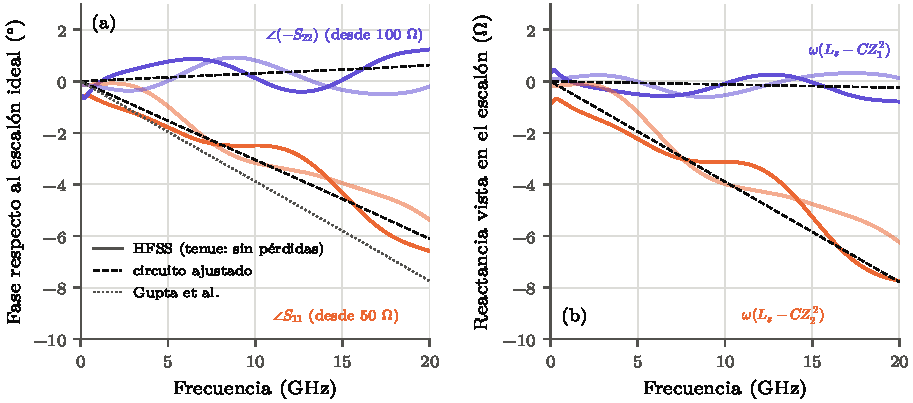
\includegraphics[width=\textwidth]{figuras/fig_d2_fase_reactancia.pdf}
\caption{Escalón: (a) fase de la reflexión respecto al escalón ideal, desde cada lado, y (b) reactancia vista en el plano del escalón desde cada lado, $\mathrm{Im}\{Z_{\mathrm{ent}}\}$. Trazo intenso: diseño con pérdidas; tenue: sin pérdidas. Las líneas discontinuas son el circuito ajustado y la punteada las fórmulas de Gupta et al.}
\label{fig:dfase}
\end{figure}

\begin{table}[htbp]
\centering
\caption{Escalón: circuito equivalente ajustado entre 1 y \SI{20}{GHz} ($L_1=<<D2_ALFA>>\,L_s$).}
\label{tab:dfit}
\small
\begin{tabular}{lcccc}
\toprule
 & $C$ (fF) & $L_s=L_1+L_2$ (pH) & $k$ & Residuo rms \\
\midrule
<<D2_FITROWS>>
Gupta et al.\ \eqref{eq:gupta} & <<D2_CGUP>> & <<D2_LGUP>> & --- & --- \\
\bottomrule
\end{tabular}
\end{table}

El valor de $k$ (<<D2_KFIT>>) indica que el escalón se comporta como si el cociente $Z_2/Z_1$ fuera, en promedio, \SI{<<D2_KPCT>>}{\percent} menor que el de los puertos de HFSS. Se ve también a baja frecuencia: con las impedancias de los puertos, \eqref{eq:gamma0} daría <<D2_G0H>>, mientras que la reflexión simulada es <<D2_GB01>>, igual a la que dan las fórmulas cuasi-estáticas.

\subsubsection{Transmisión y pérdida de inserción}
La transmisión del escalón es $|S_{21}|\approx\SI{-<<D2_ILB01>>}{dB}$ en toda la banda (Figura~\ref{fig:dsdb}b), y coincide con el límite $10\log_{10}(1-\Gamma_0^2)=\SI{-<<D2_ILR0Q>>}{dB}$: toda su pérdida de inserción es potencia reflejada. La transición gradual pierde \SI{<<D2_ILC10>>}{dB} a \SI{10}{GHz} y \SI{<<D2_ILC20>>}{dB} a \SI{20}{GHz}, y esa pérdida ya casi no es reflexión. La separación \eqref{eq:separacion}, aplicada a los parámetros corregidos, se muestra en la Figura~\ref{fig:dpot} y en la Tabla~\ref{tab:dpot}: ninguna de las dos estructuras radia más de \SI{<<D2_PRADCMAX>>}{\percent}, que está en el orden de la incertidumbre ($\pm\SI{<<D2_PISO2>>}{\percent}$, tomada del valor negativo más grande que da la estimación). El escalón tampoco disipa de forma apreciable (\SI{<<D2_PDISB20>>}{\percent} a \SI{20}{GHz}). La transición sí disipa (\SI{<<D2_PDISC10>>}{\percent} a \SI{10}{GHz} y \SI{<<D2_PDISC20>>}{\percent} a \SI{20}{GHz}), porque agrega \SI{10}{mm} de línea; la atenuación promedio de las dos líneas, calculada con la constante de propagación de HFSS, da \SI{<<D2_PDISLIN10>>}{\percent} y \SI{<<D2_PDISLIN20>>}{\percent} para esa longitud.

\begin{figure}[htbp]
\centering
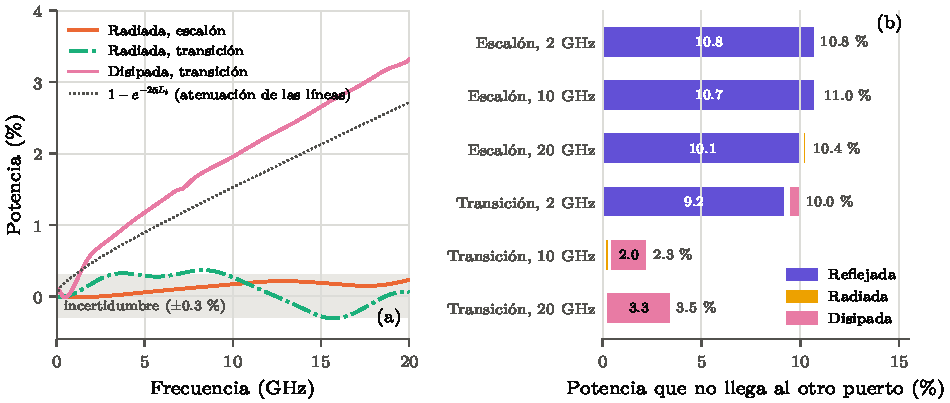
\includegraphics[width=\textwidth]{figuras/fig_d2_potencia.pdf}
\caption{Cambio de ancho: (a) potencia radiada (escalón y transición) y disipada (transición), con la banda de incertidumbre de la radiada; la línea punteada es la pérdida esperada por la atenuación de las líneas. (b) Destino de la potencia que no llega al otro puerto.}
\label{fig:dpot}
\end{figure}

\begin{table}[htbp]
\centering
\caption{Cambio de ancho: destino de la potencia incidente (\%), con parámetros corregidos. Reflejada: promedio de $|S_{11}|^2$ y $|S_{22}|^2$.}
\label{tab:dpot}
\small
\setlength{\tabcolsep}{4pt}
\begin{tabular}{lccccccc}
\toprule
Diseño & $f$ (GHz) & Transmitida & Reflejada & Radiada & Disipada & IL (dB) & IL$_{\mathrm{refl}}$ (dB) \\
\midrule
<<D2_POWROWS2>>
\bottomrule
\end{tabular}
\end{table}

\subsection{Discusión: explicación física}

\subsubsection{Por qué el cambio de ancho refleja}
Una línea de transmisión impone un cociente fijo entre el voltaje y la corriente de la onda que viaja por ella, $Z_0=\sqrt{L'/C'}$, y ese cociente lo fija la sección transversal. La onda que llega por la línea ancha trae $V/I=\SI{50}{\ohm}$. En la unión el voltaje y la corriente deben ser continuos, pero la línea angosta, con la mitad de capacitancia y casi el doble de inductancia por unidad de longitud, solo puede llevar ondas con $V/I=\SI{100}{\ohm}$. La única forma de cumplir ambas condiciones es que parte de la onda regrese, y la proporción la fija \eqref{eq:gamma0}. Ningún elemento de esta explicación depende de la frecuencia: depende del cociente de las secciones transversales, no de una longitud comparada con $\lambda_g$.

\begin{figure}[htbp]
\centering
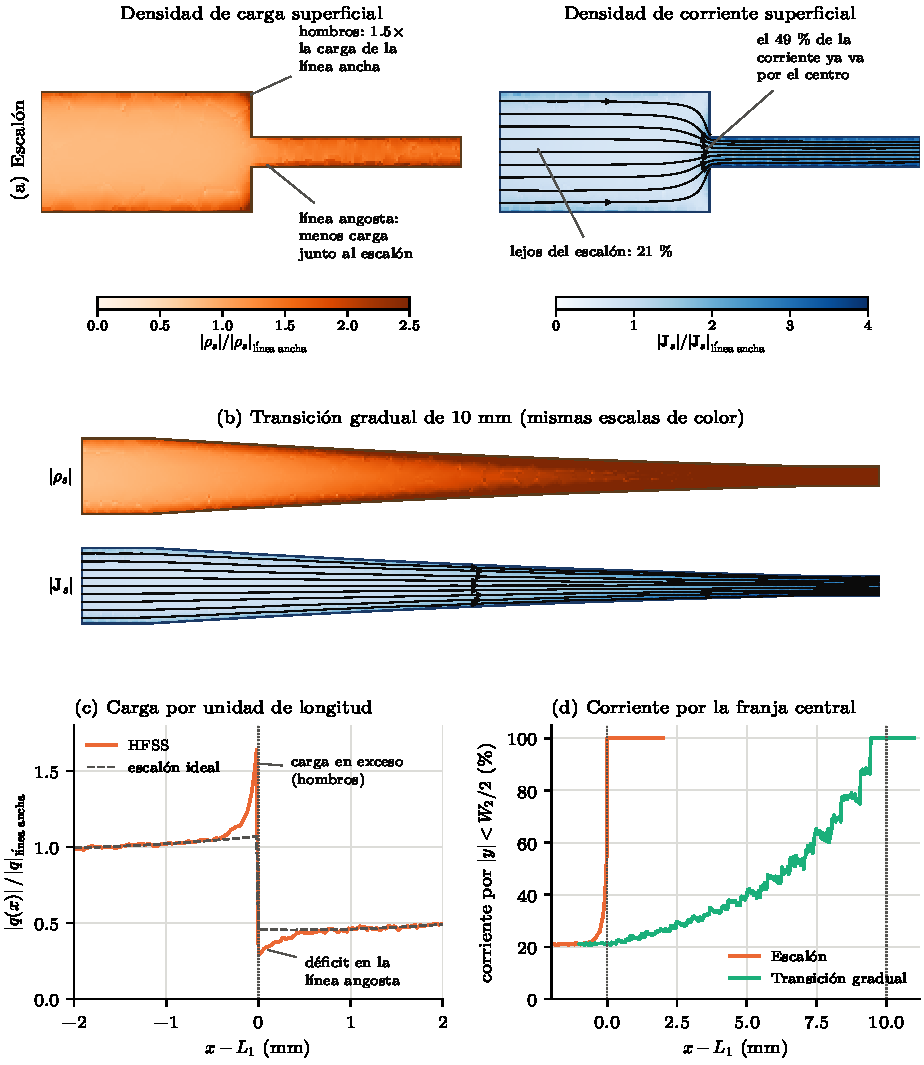
\includegraphics[width=\textwidth]{figuras/fig_d2_carga_corriente.pdf}
\caption{Cambio de ancho a \SI{5}{GHz}, calculado con \eqref{eq:saltos} a partir de los campos de HFSS: (a) densidad de carga y de corriente superficiales en el escalón, normalizadas a su promedio en la línea ancha lejos del escalón, con las líneas de flujo de la corriente; (b) lo mismo en la transición gradual; (c) carga por unidad de longitud $|q(x)|=|\int\rho_s\,dy|$ a lo largo del escalón, frente a un escalón ideal (extrapolación de cada línea hasta el plano de unión); (d) fracción de la corriente que circula por la franja central $|y|<W_2/2$.}
\label{fig:dcarga}
\end{figure}

Los campos de HFSS muestran además los elementos parásitos (Figura~\ref{fig:dcarga}a y c). La parte de la tira ancha que no continúa termina como un extremo abierto: su borde frontal tiene campo de borde hacia el plano de tierra y concentra carga en los hombros del escalón, <<D2_CHOM>> veces la de la línea ancha. Inmediatamente después, la línea angosta tiene menos carga que en su tramo uniforme, porque parte de su campo termina en el frente de la tira ancha; ese déficit compensa en parte el exceso de los hombros. El resultado neto es la capacitancia en paralelo $C$. Al mismo tiempo, la corriente de toda la tira ancha tiene que entrar en la angosta: justo antes del escalón el <<D2_ICEN>>\,\% de la corriente ya circula por la franja central de ancho $W_2$, frente al <<D2_ICENL>>\,\% lejos de él (Figura~\ref{fig:dcarga}d). Esa concentración aumenta la energía magnética y es la inductancia serie $L_s$.

Ambos elementos son muy pequeños. $C=\SI{<<D2_CEXC>>}{fF}$ es la capacitancia de solo \SI{<<D2_DLC>>}{\micro\metre} de línea de \SI{50}{\ohm}, y $L_s=\SI{<<D2_LEXC>>}{pH}$ la inductancia de \SI{<<D2_DLL>>}{\micro\metre} de línea de \SI{100}{\ohm}. Por eso el escalón se parece tanto a la unión ideal: es como si cada línea fuera unas decenas de micrómetros más larga, una distancia despreciable frente a $\lambda_g$.

\subsubsection{A partir de qué frecuencia el efecto es significativo}
Con el mismo criterio que en la curva ($|S_{11}|>-20$~dB), el escalón es significativo \textbf{en toda la banda, desde las frecuencias más bajas}: su reflexión de \SI{<<D2_S11B01>>}{dB} está 10~dB por encima del umbral ya a \SI{0.1}{GHz}. No existe una frecuencia a partir de la cual ``aparezca'', porque la desadaptación no depende de $\omega$. Esta es la diferencia de fondo con la curva, cuya reflexión se debe solo a la reactancia parásita y por eso es nula a baja frecuencia.

Lo que sí depende de la frecuencia es la contribución de los parásitos. Por \eqref{eq:zent}, desde la línea de \SI{50}{\ohm} el escalón ve la reactancia $X_1=\omega(L_s-CZ_2^2)$, con $CZ_2^2\approx\SI{<<D2_CZ2>>}{pH}$ frente a $L_s\approx\SI{<<D2_LEXC>>}{pH}$: domina la capacitancia y $X_1\approx\omega\cdot(\SI{<<D2_X1>>}{pH})$. Esa reactancia solo llegaría al 10\,\% de $Z_2$ hacia \SI{<<D2_F10X>>}{GHz}, fuera de la banda; dentro de ella solo gira la fase de $\Gamma$, unos \ang{<<D2_ANGB20ABS>>} a \SI{20}{GHz}, de acuerdo con \eqref{eq:fase_escalon}. Desde la línea de \SI{100}{\ohm} la reactancia es $\omega(L_s-CZ_1^2)$ con $CZ_1^2\approx\SI{<<D2_CZ1>>}{pH}\approx L_s$: la capacitancia y la inductancia casi se cancelan y el escalón se ve prácticamente ideal. La misma capacitancia pesa distinto según el lado porque un elemento en paralelo importa en proporción a la impedancia del circuito en que está conectado: frente a la carga de \SI{100}{\ohm} su efecto es cuatro veces mayor que frente a la de \SI{50}{\ohm}.

\begin{figure}[htbp]
\centering
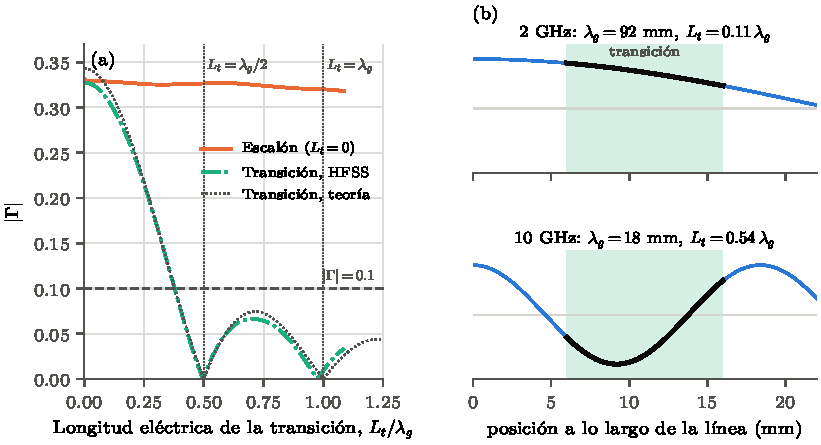
\includegraphics[width=\textwidth]{figuras/fig_d2_escala.pdf}
\caption{(a) Reflexión de la transición gradual en función de su longitud eléctrica $L_t/\lambda_g$ (HFSS y \eqref{eq:taper}), junto con la del escalón ($L_t=0$). (b) Instantánea de la onda guiada a lo largo de la estructura a 2 y \SI{10}{GHz}; la franja es la transición y el tramo negro la parte de la onda que cae dentro de ella.}
\label{fig:descala}
\end{figure}

\subsubsection{Por qué la transición gradual solo funciona a alta frecuencia}
Una transición se puede ver como muchos escalones pequeños en cascada, cada uno con una reflexión $d\Gamma=\frac{1}{2}d(\ln Z)$; la reflexión total es la suma de todas ellas con la fase del recorrido de ida y vuelta hasta cada una, y de ahí sale \eqref{eq:taper}. La Figura~\ref{fig:descala} muestra lo que eso significa. A \SI{2}{GHz} ($\lambda_g=\SI{<<D2_LG2T>>}{mm}$) la transición mide $<<D2_LTLG2>>\,\lambda_g$: la onda casi no cambia a lo largo de ella, todas las reflexiones parciales llegan en fase y se suman, y la transición refleja lo mismo que el escalón. Para la onda, a esa frecuencia, \SI{10}{mm} siguen siendo un cambio brusco. A \SI{10}{GHz} ($\lambda_g=\SI{<<D2_LG10T>>}{mm}$) la transición mide $<<D2_LTLG10>>\,\lambda_g$: las reflexiones parciales de su primera y su segunda mitad llegan con fases opuestas y se cancelan. En HFSS la reflexión baja de $-20$~dB cuando la transición mide $<<D2_LTLGU>>\,\lambda_g$ (\SI{<<D2_FT20>>}{GHz}) y se anula en $L_t=\lambda_g/2$ y $L_t=\lambda_g$, como predice la teoría.

``Abrupto'' significa entonces corto frente a $\lambda_g/2$, y no tiene que ver con la forma de la unión. La transición tiene dos costos: ocupa espacio y agrega pérdidas en proporción a su longitud (\SI{<<D2_PDISC20>>}{\percent} disipado a \SI{20}{GHz}). Ninguna transición de longitud finita puede corregir el desacople a frecuencias suficientemente bajas; para eso hace falta una red de acoplamiento, como un transformador de $\lambda/4$, que a su vez solo funciona en una banda.

Por último, ni el escalón ni la transición radian de forma apreciable. A diferencia de la curva, la corriente no cambia de dirección: la tira y su imagen en el plano de tierra siguen formando un par de corrientes opuestas y alineadas (Sección~\ref{sec:d1rad}), y sus campos lejanos se siguen cancelando.

%======================================================================
\section{Discontinuidad 3: gap en serie}
\label{sec:d3}

\subsection{Diseño y estructuras simuladas}
Se interrumpió la línea de \SI{50}{\ohm} con un corte de ancho $s$ (Figura~\ref{fig:d3geo}). A diferencia de las discontinuidades anteriores, aquí el tamaño del corte cambia por completo el comportamiento, así que se simularon cinco separaciones: $s=0.1$, 0.2, 0.5 y \SI{1}{mm} ($s/W$ entre 0.09 y 0.88, el rango de las fórmulas de Garg y Bahl) y $s=\SI{3}{mm}$, donde el acoplamiento es despreciable y cada lado se comporta como un extremo abierto. Los planos de referencia se colocaron, tras el de-embedding de $L_1$, en las caras de los dos extremos, de modo que entre ellos solo queda el corte. Como en las otras discontinuidades, cada estructura tiene su gemelo sin pérdidas, y se repitió la línea recta de referencia, con y sin pérdidas, para corregir el error de los puertos (Sección~\ref{sec:correccion}). La Figura~\ref{fig:d3hfss} muestra los modelos tal como quedaron en HFSS.

\begin{figure}[htbp]
\centering
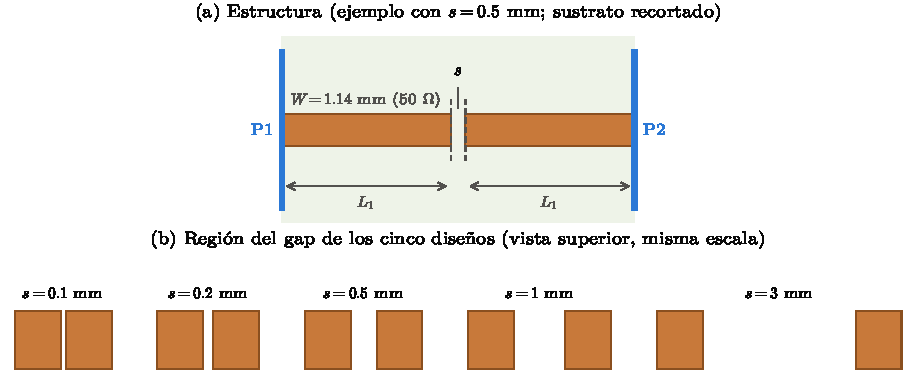
\includegraphics[width=\textwidth]{figuras/fig_d3_geometria.pdf}
\caption{Gap en serie: (a) estructura completa, con los planos de referencia en las caras de los extremos; (b) región del corte de los cinco diseños a la misma escala.}
\label{fig:d3geo}
\end{figure}

\begin{figure}[htbp]
\centering
\begin{subfigure}[b]{0.32\textwidth}
\centering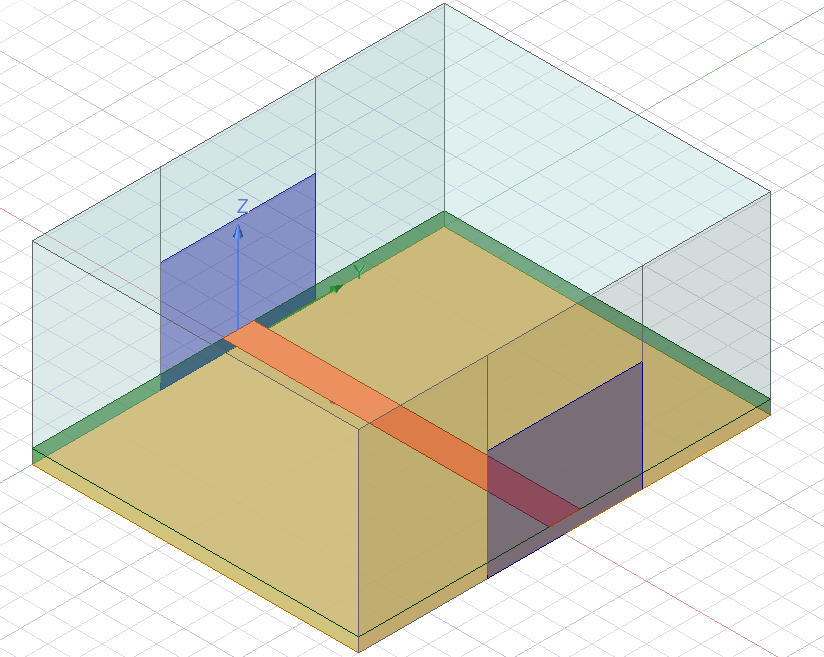
\includegraphics[width=\linewidth]{figuras/hfss3d_d3_ref.png}
\caption{Referencia}
\end{subfigure}\hfill
\begin{subfigure}[b]{0.32\textwidth}
\centering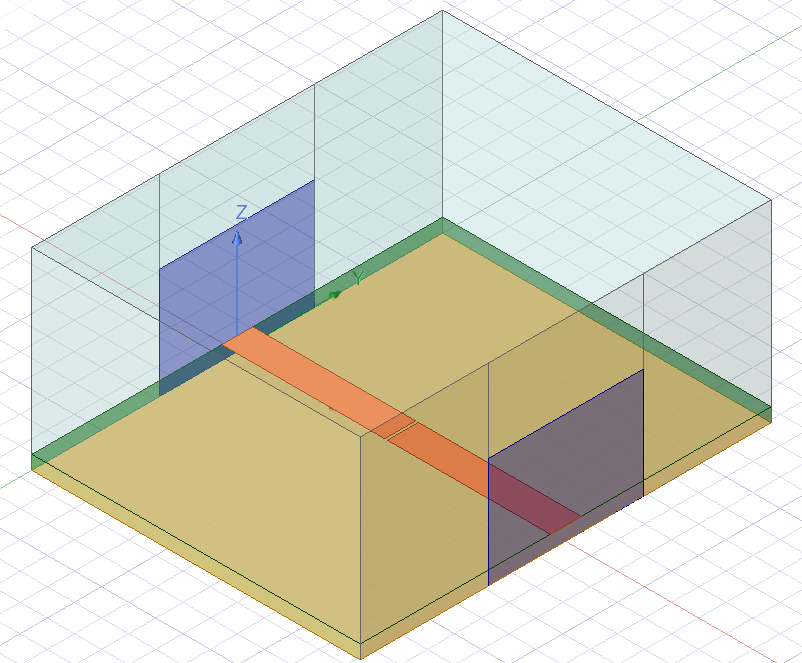
\includegraphics[width=\linewidth]{figuras/hfss3d_d3_0p1.png}
\caption{$s=\SI{0.1}{mm}$}
\end{subfigure}\hfill
\begin{subfigure}[b]{0.32\textwidth}
\centering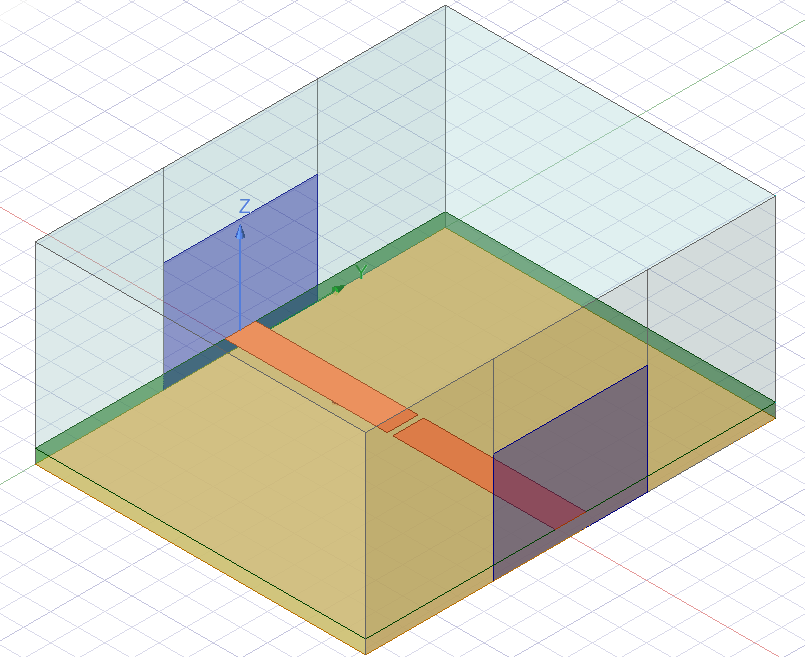
\includegraphics[width=\linewidth]{figuras/hfss3d_d3_0p2.png}
\caption{$s=\SI{0.2}{mm}$}
\end{subfigure}\\[6pt]
\begin{subfigure}[b]{0.32\textwidth}
\centering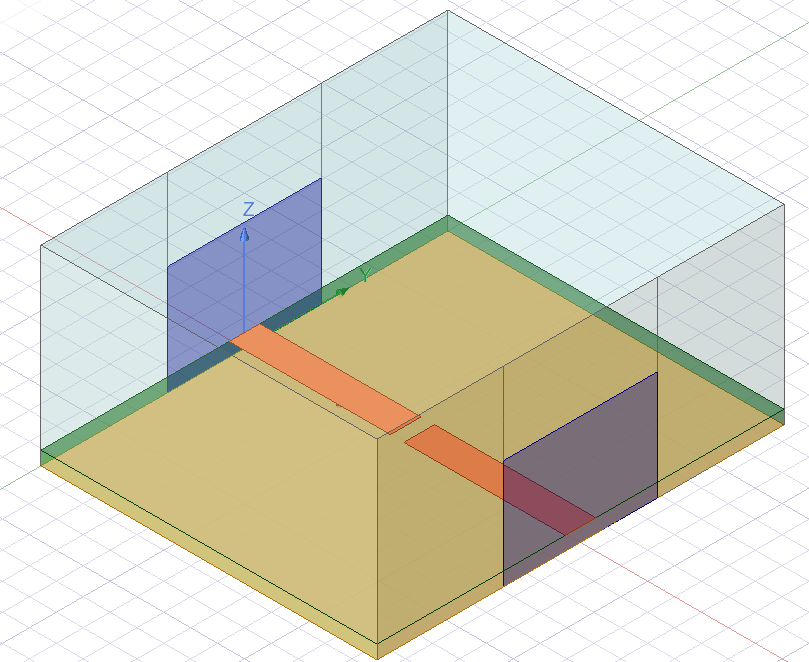
\includegraphics[width=\linewidth]{figuras/hfss3d_d3_0p5.png}
\caption{$s=\SI{0.5}{mm}$}
\end{subfigure}\hfill
\begin{subfigure}[b]{0.32\textwidth}
\centering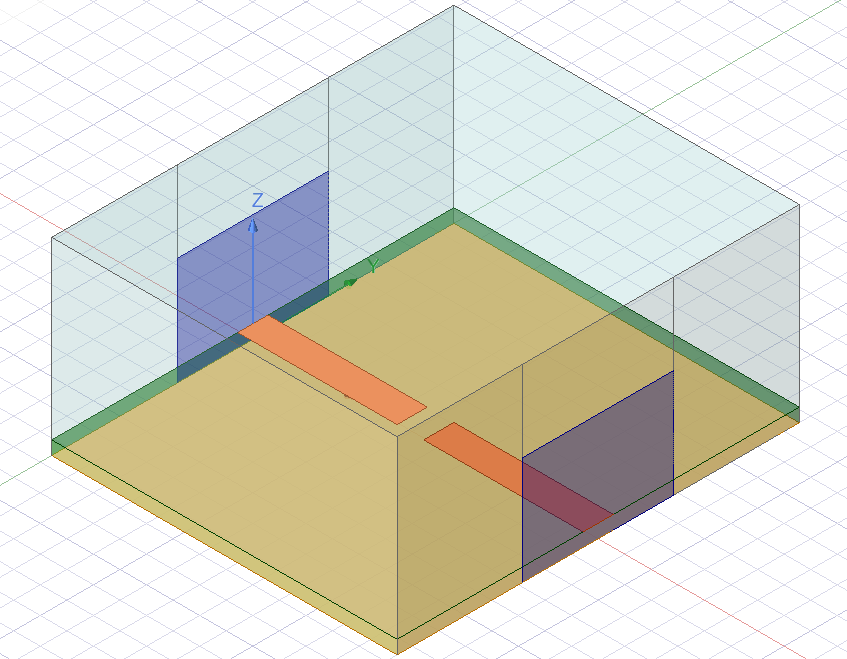
\includegraphics[width=\linewidth]{figuras/hfss3d_d3_1p0.png}
\caption{$s=\SI{1}{mm}$}
\end{subfigure}\hfill
\begin{subfigure}[b]{0.32\textwidth}
\centering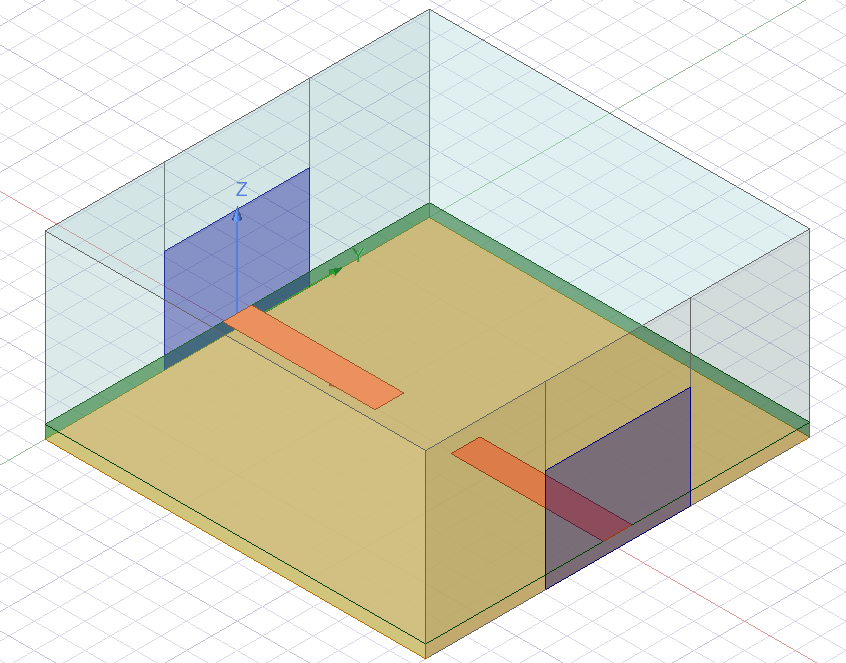
\includegraphics[width=\linewidth]{figuras/hfss3d_d3_3p0.png}
\caption{$s=\SI{3}{mm}$}
\end{subfigure}
\caption{Modelos 3D del gap en serie en HFSS: la línea de referencia y las cinco separaciones, con la misma caja de aire y los mismos puertos que las demás discontinuidades.}
\label{fig:d3hfss}
\end{figure}

\paragraph{Tratamiento numérico.} Los parámetros $S$ se corrigieron con las cajas de error de la línea de referencia, igual que en el cambio de ancho; el residuo de la referencia corregida es $|S_{11}|\leq <<D3_RESREF3>>$. El circuito $\pi$ se extrajo directamente con \eqref{eq:ygap}: a diferencia del escalón, aquí $Y_{21}$ es pequeño pero no despreciable y no hay una conexión directa que amplifique los errores. $C_g$ y $C_p$ se promediaron entre 3 y \SI{15}{GHz}, y su incertidumbre es la mayor entre la diferencia de los gemelos con y sin pérdidas y la variación con la frecuencia en esa banda.

\subsection{Resultados}

\subsubsection{Reflexión y transmisión}
El gap refleja casi toda la potencia en toda la banda: $|S_{11}|\geq <<D3_GMIN3>>$ en todos los casos (Tabla~\ref{tab:d3sparam}). Lo que distingue a los cinco diseños es la transmisión (Figura~\ref{fig:d3s}a). En escala logarítmica de frecuencia, $|S_{21}|$ es una recta con pendiente de <<D3_PENDMIN>> a <<D3_PENDMAX>>~dB por década entre 1 y \SI{10}{GHz}, como predice \eqref{eq:sgap} para un capacitor en serie. Con $s=\SI{0.1}{mm}$ la transmisión pasa de \SI{<<D3_S21G1_1>>}{dB} a \SI{1}{GHz} a \SI{<<D3_S21G1_20>>}{dB} a \SI{20}{GHz}, y supera el 10\,\% de la potencia ($-10$~dB) a partir de \SI{<<D3_F10DB>>}{GHz}. Con $s=\SI{0.2}{mm}$ llega a \SI{<<D3_S21G2_20>>}{dB} a \SI{20}{GHz}; con $s=\SI{1}{mm}$, a \SI{<<D3_S21G4_20>>}{dB}; y con $s=\SI{3}{mm}$ no pasa de \SI{<<D3_S21G5_20>>}{dB}. La fase de $S_{11}$ (Figura~\ref{fig:d3s}b) se aleja de la de un circuito abierto ideal en proporción a la frecuencia: el extremo almacena carga, y eso equivale a un circuito abierto situado un poco más allá de él.

\begin{figure}[htbp]
\centering
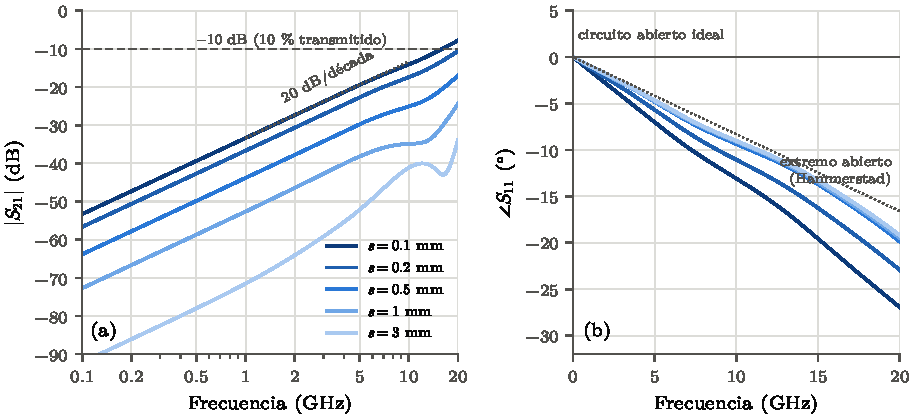
\includegraphics[width=\textwidth]{figuras/fig_d3_S.pdf}
\caption{Gap en serie: (a) transmisión en escala logarítmica de frecuencia, con la pendiente de 20~dB por década como guía; (b) fase de $S_{11}$, junto con la de un extremo abierto de longitud equivalente \eqref{eq:dloc}.}
\label{fig:d3s}
\end{figure}

\begin{table}[htbp]
\centering
\caption{Gap en serie: $|\Gamma|=|S_{11}|$ y $|S_{21}|$ (dB) en frecuencias seleccionadas.}
\label{tab:d3sparam}
\small
\setlength{\tabcolsep}{3.4pt}
\begin{tabular}{c cc cc cc cc cc}
\toprule
 & \multicolumn{2}{c}{$s=\SI{0.1}{mm}$} & \multicolumn{2}{c}{$s=\SI{0.2}{mm}$} & \multicolumn{2}{c}{$s=\SI{0.5}{mm}$} & \multicolumn{2}{c}{$s=\SI{1}{mm}$} & \multicolumn{2}{c}{$s=\SI{3}{mm}$} \\
\cmidrule(lr){2-3}\cmidrule(lr){4-5}\cmidrule(lr){6-7}\cmidrule(lr){8-9}\cmidrule(lr){10-11}
$f$ (GHz) & $|\Gamma|$ & $S_{21}$ & $|\Gamma|$ & $S_{21}$ & $|\Gamma|$ & $S_{21}$ & $|\Gamma|$ & $S_{21}$ & $|\Gamma|$ & $S_{21}$ \\
\midrule
<<D3_SROWS3>>
\bottomrule
\end{tabular}
\end{table}

Con una reflexión tan grande, el VSWR deja de ser una figura útil: con $s=\SI{0.1}{mm}$ vale <<D3_VSWRG1_20>> a \SI{20}{GHz}, donde todavía se refleja el <<D3_PR1_20>>\,\% de la potencia, y en los demás casos es aún mayor.

\subsubsection{Circuito equivalente}
La Figura~\ref{fig:d3cap} y la Tabla~\ref{tab:d3circ} muestran los elementos de la red $\pi$. Ambos son prácticamente constantes con la frecuencia (Figura~\ref{fig:d3cap}b), como corresponde a elementos concentrados, y cambian con la separación en sentidos opuestos: $C_g$ cae de \SI{<<D3_CG0P1>>}{fF} con $s=\SI{0.1}{mm}$ a menos de \SI{1}{fF} con $s=\SI{3}{mm}$, mientras que $C_p$ crece de \SI{<<D3_CP0P1>>}{} a \SI{<<D3_CP3P0>>}{fF}. Para $s\geq\SI{0.5}{mm}$ la suma $C_g+C_p$ se mantiene en unos \SI{<<D3_CT1P0>>}{fF}: la carga del extremo es la misma, y solo cambia hacia dónde van sus líneas de campo. Con $s=\SI{3}{mm}$, $C_p$ corresponde a una extensión de \SI{<<D3_DLEXT>>}{mm}, frente a \SI{<<D3_DLOC>>}{mm} de la fórmula de Hammerstad \eqref{eq:dloc} (\SI{<<D3_COC>>}{fF}). Las fórmulas de Garg y Bahl reproducen la tendencia de ambas capacitancias, pero dan $C_g$ entre <<D3_RGBMIN>> y <<D3_RGBMAX>> veces menor que HFSS; hay que notar que el sustrato está ligeramente fuera de su rango ($W/h=2.24>2$).

\begin{figure}[htbp]
\centering
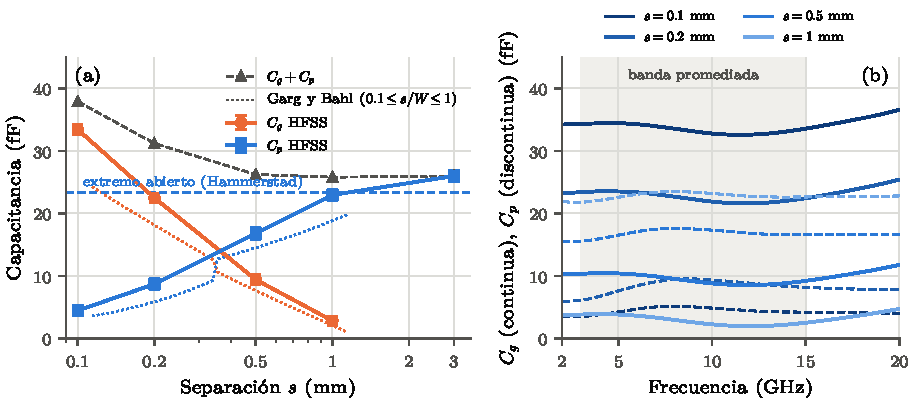
\includegraphics[width=\textwidth]{figuras/fig_d3_capacitancias.pdf}
\caption{Gap en serie: (a) $C_g$ y $C_p$ extraídas de HFSS en función de la separación, frente a las fórmulas de Garg y Bahl \eqref{eq:gargbahl} y al extremo abierto \eqref{eq:dloc}; (b) $C_g$ y $C_p$ en función de la frecuencia (diseños con pérdidas).}
\label{fig:d3cap}
\end{figure}

\begin{table}[htbp]
\centering
\caption{Gap en serie: circuito $\pi$ extraído de HFSS (promedio de 3 a \SI{15}{GHz}) y fórmulas cerradas. $f_c=1/(2\pi\cdot 2Z_0C_g)$ es la frecuencia a la que la reactancia de $C_g$ iguala a $2Z_0$.}
\label{tab:d3circ}
\small
\begin{tabular}{cccccccc}
\toprule
 & & \multicolumn{2}{c}{HFSS (fF)} & \multicolumn{2}{c}{Garg y Bahl (fF)} & \\
\cmidrule(lr){3-4}\cmidrule(lr){5-6}
$s$ (mm) & $s/W$ & $C_g$ & $C_p$ & $C_g$ & $C_p$ & $f_c$ (GHz) \\
\midrule
<<D3_CIRCROWS>>
\bottomrule
\multicolumn{7}{l}{\footnotesize $^{\ddagger}$Capacitancia del extremo abierto, \eqref{eq:dloc}.}
\end{tabular}
\end{table}

\subsubsection{Potencia}
La potencia que ni se refleja ni se transmite (Figura~\ref{fig:d3pot} y Tabla~\ref{tab:d3pot}) es casi toda radiación: la disipación no pasa de \SI{<<D3_PDISMAX3>>}{\percent}. La radiación es prácticamente la misma para todas las separaciones: unos \SI{<<D3_PRAD5>>}{\percent} a \SI{5}{GHz}, \SI{<<D3_PRAD10>>}{\percent} a \SI{10}{GHz} y entre \SI{<<D3_PRAD20MIN>>}{} y \SI{<<D3_PRAD20MAX>>}{\percent} a \SI{20}{GHz}, y supera el 1\,\% a partir de unos \SI{<<D3_F1PCT>>}{GHz}. Su incertidumbre es mayor que en las otras discontinuidades ($\pm\SI{<<D3_PISO3>>}{\percent}$): con $|S_{11}|\approx 1$, cualquier error en $|S_{11}|$ aparece casi al doble en $|S_{11}|^2$.

\begin{figure}[htbp]
\centering
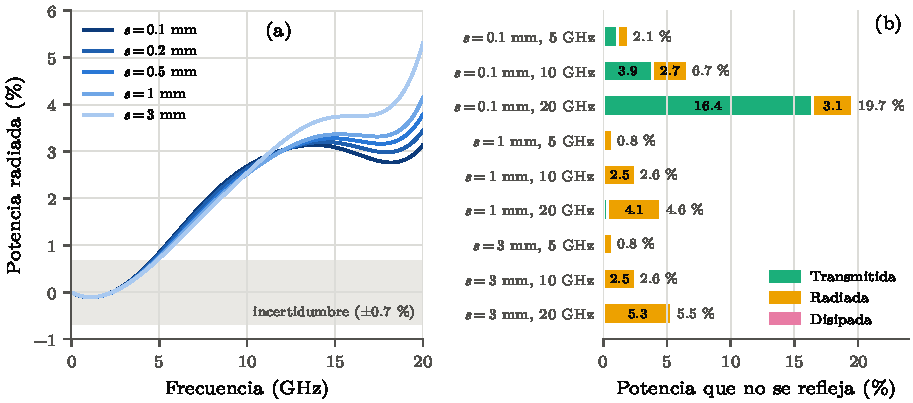
\includegraphics[width=\textwidth]{figuras/fig_d3_potencia.pdf}
\caption{Gap en serie: (a) potencia radiada (gemelos sin pérdidas, corregidos), con la banda de incertidumbre; (b) destino de la potencia que no se refleja.}
\label{fig:d3pot}
\end{figure}

\begin{table}[htbp]
\centering
\caption{Gap en serie: destino de la potencia incidente (\%), con parámetros corregidos.}
\label{tab:d3pot}
\small
\begin{tabular}{lccccc}
\toprule
Diseño & $f$ (GHz) & Reflejada & Transmitida & Radiada & Disipada \\
\midrule
<<D3_POWROWS3>>
\bottomrule
\end{tabular}
\end{table}

\subsection{Discusión: explicación física}

\subsubsection{Por qué el gap refleja casi todo}
En el extremo de la tira la corriente de conducción tiene que anularse, porque no tiene a dónde ir. Una onda que llega con corriente distinta de cero solo puede cumplir esa condición si se superpone con una onda reflejada de casi la misma amplitud: se forma una onda estacionaria con un nodo de corriente y un máximo de voltaje en el extremo. Ese voltaje carga el extremo, y la carga produce un campo eléctrico que se reparte entre el plano de tierra ($C_p$) y el extremo de enfrente ($C_g$). Solo la segunda parte cruza el corte: induce en el otro extremo una carga de signo opuesto, y su variación en el tiempo es la corriente de desplazamiento que alimenta la segunda línea.

\begin{figure}[htbp]
\centering
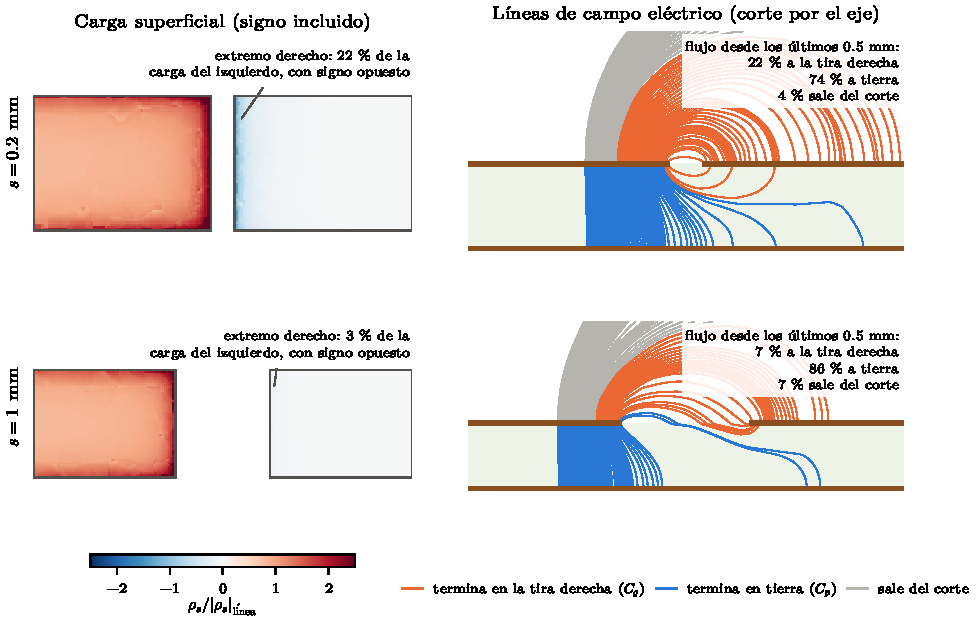
\includegraphics[width=\textwidth]{figuras/fig_d3_campos.pdf}
\caption{Gap en serie a \SI{5}{GHz}, a partir de los campos de HFSS, para $s=\SI{0.2}{mm}$ (arriba) y $s=\SI{1}{mm}$ (abajo). Izquierda: densidad de carga superficial con su signo, normalizada a la de la línea a \SI{1.25}{mm} del extremo, en la fase en que la carga del extremo es máxima. Derecha: líneas de campo eléctrico en el plano vertical que pasa por el eje de la línea, trazadas desde los últimos \SI{0.5}{mm} de la tira izquierda y clasificadas por su destino; los porcentajes están pesados por el flujo de $\mathbf{D}$ en el punto de partida.}
\label{fig:d3campos}
\end{figure}

La Figura~\ref{fig:d3campos} muestra este reparto. Con $s=\SI{0.2}{mm}$, el último medio milímetro de la tira derecha tiene una carga de signo opuesto igual al <<D3_RQ02>>\,\% de la del último medio milímetro de la izquierda; con $s=\SI{1}{mm}$, solo el <<D3_RQ10>>\,\%. Con el circuito extraído, ese cociente debería ser $C_g/(C_g+C_p+C'\ell)$, donde $C'\ell$ es la capacitancia del tramo de línea de longitud $\ell=\SI{0.5}{mm}$, lo que da <<D3_RC02>>\,\% y <<D3_RC10>>\,\%; la coincidencia es razonable, considerando que el cálculo con campos incluye la carga distribuida exacta cerca del extremo y el circuito no. Las líneas de campo cuentan lo mismo de forma visual: con el gap pequeño una parte importante del flujo que sale de la tira izquierda termina en la derecha (en este corte, <<D3_FL02>>\,\%), y con el gap grande casi todo baja a tierra.

\subsubsection{A partir de qué frecuencia el efecto es significativo}
Con el criterio de las otras discontinuidades, el gap es significativo en toda la banda y desde DC: a frecuencia cero es un circuito abierto, y aun a \SI{20}{GHz} refleja al menos el <<D3_PR1_20>>\,\% de la potencia. Lo que sí depende de la frecuencia es cuánto deja pasar. Por \eqref{eq:sgap}, la transmisión es proporcional a $\omega C_g$: la corriente de desplazamiento a través de un capacitor crece con la rapidez con que cambia el voltaje. El gap solo se volvería ``transparente'' cuando la reactancia de $C_g$ fuera pequeña frente a $2Z_0$, y la Tabla~\ref{tab:d3circ} muestra que eso ocurre hasta \SI{<<D3_FCORTE0P1>>}{GHz} para el gap más angosto y \SI{<<D3_FCORTE0P2>>}{GHz} para el de \SI{0.2}{mm}, muy por encima de la banda. Por eso un simple corte en la pista es un mal capacitor de bloqueo de DC a estas frecuencias: para ese uso se emplean capacitores interdigitales o líneas acopladas, que ponen mucha más longitud de borde frente a frente para aumentar $C_g$.

Con la frecuencia también crece la radiación. A diferencia de la curva, aquí no la produce un cambio de dirección de la corriente, sino el extremo abierto mismo: el campo de borde entre el extremo y el plano de tierra forma una pequeña abertura radiante, la misma que aprovechan los bordes de una antena de parche. Además lanza ondas de superficie dentro del sustrato, que en la simulación se cuentan como potencia que sale del dominio. Como el extremo izquierdo está igual de cargado en todos los diseños (la reflexión es casi total en todos), la radiación casi no depende de $s$.

%======================================================================
\section{Discontinuidad 4: cambio de material a mitad de la línea}
\label{sec:d4}

\subsection{Diseño y estructuras simuladas}
La línea de \SI{50}{\ohm} sobre RO4003C continúa, a partir de $x=L_1$, sobre otro material, sin cambiar su forma (Figura~\ref{fig:d4geo}). Un cambio de material puede ocurrir de dos maneras, y se simularon ambas:
\begin{itemize}
\item \textbf{Cambio de sustrato.} La tira de cobre de \SI{1.14}{mm} pasa sobre un sustrato del mismo espesor, pero de otro material: FR-4 ($\varepsilon_r=4.4$, $\tan\delta=0.02$), el laminado de bajo costo más común, y Rogers RO3010 ($\varepsilon_r=10.2$, $\tan\delta=0.0022$) \cite{rogers3000}, un laminado de alta permitividad que da un contraste grande y deja ver el efecto con claridad.
\item \textbf{Cambio de metal.} El sustrato no cambia, pero la segunda mitad de la tira es de estaño ($\sigma=\SI{8.7}{MS/m}$, contra \SI{58}{MS/m} del cobre), como en un tramo estañado o una zona de soldadura.
\end{itemize}
Además se simuló una variante compensada del cambio a RO3010, con la tira de la segunda mitad reducida a \SI{0.48}{mm} para que esa línea también sea de \SI{50}{\ohm}. No es otra discontinuidad de ancho: sirve para separar qué parte de la reflexión se debe a la diferencia de impedancias y qué parte a la frontera entre los dos materiales, y es lo que se hace en la práctica cuando una línea tiene que pasar de un laminado a otro.

Cada puerto se refirió a la impedancia de su propia línea y, tras el de-embedding de $L_1$, ambos planos de referencia quedaron en la unión, de modo que los parámetros $S$ describen solo la frontera entre materiales y no las pérdidas de los tramos de alimentación. Para corregir el error de los puertos hace falta una línea de referencia por cada tipo de línea que toca un puerto: RO4003C con cobre (puerto 1 de todos los diseños), FR-4, RO3010, RO3010 con la tira de \SI{0.48}{mm} y RO4003C con estaño. Los diseños con cambio de sustrato tienen su gemelo sin pérdidas; el cambio de metal no, porque sin pérdidas el cobre y el estaño son el mismo conductor perfecto. En total se resolvieron <<D4_NDIS4>> diseños (Figura~\ref{fig:d4hfss}).

\begin{figure}[htbp]
\centering
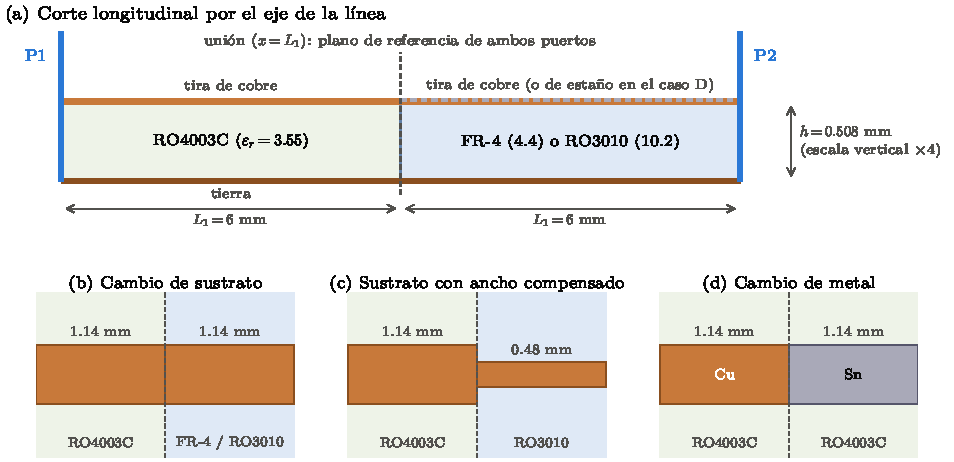
\includegraphics[width=\textwidth]{figuras/fig_d4_geometria.pdf}
\caption{Cambio de material: (a) corte longitudinal, con los dos sustratos y los planos de referencia en la unión; (b)--(d) vista superior de la zona de la unión en los tres casos simulados.}
\label{fig:d4geo}
\end{figure}

\begin{figure}[htbp]
\centering
\begin{subfigure}[b]{0.32\textwidth}
\centering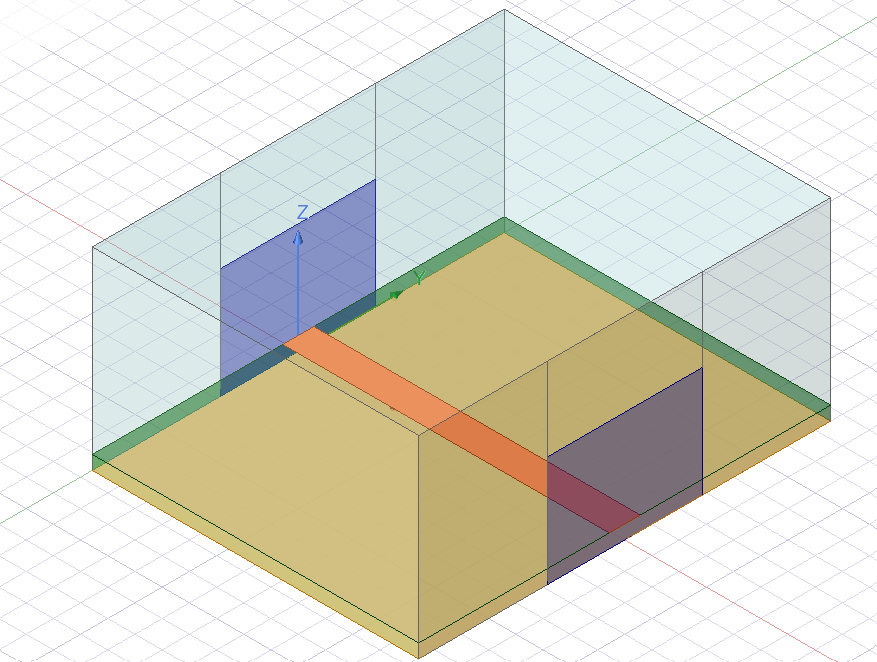
\includegraphics[width=\linewidth]{figuras/hfss3d_d4_ref.png}
\caption{Referencia (un solo material)}
\end{subfigure}\hfill
\begin{subfigure}[b]{0.32\textwidth}
\centering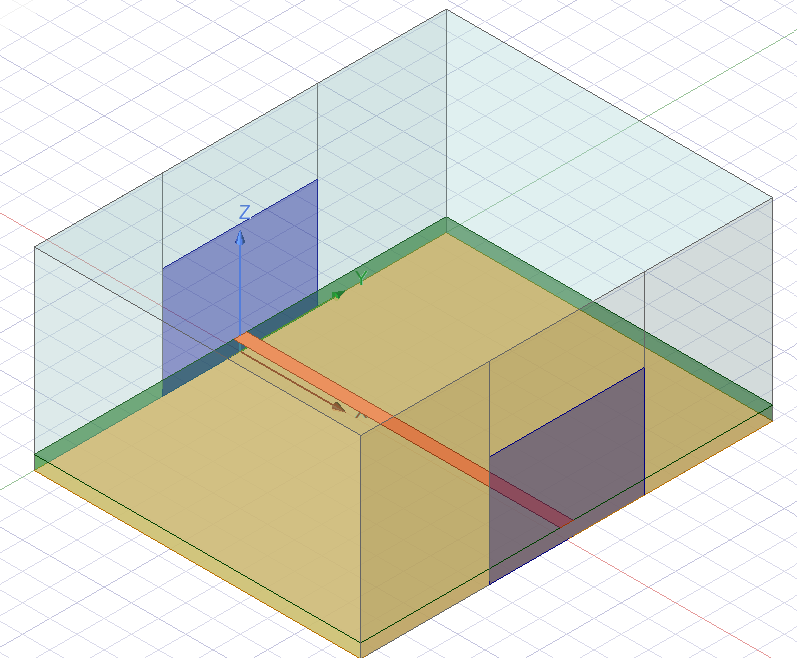
\includegraphics[width=\linewidth]{figuras/hfss3d_d4_ref_w50.png}
\caption{Referencia RO3010, $W=\SI{0.48}{mm}$}
\end{subfigure}\hfill
\begin{subfigure}[b]{0.32\textwidth}
\centering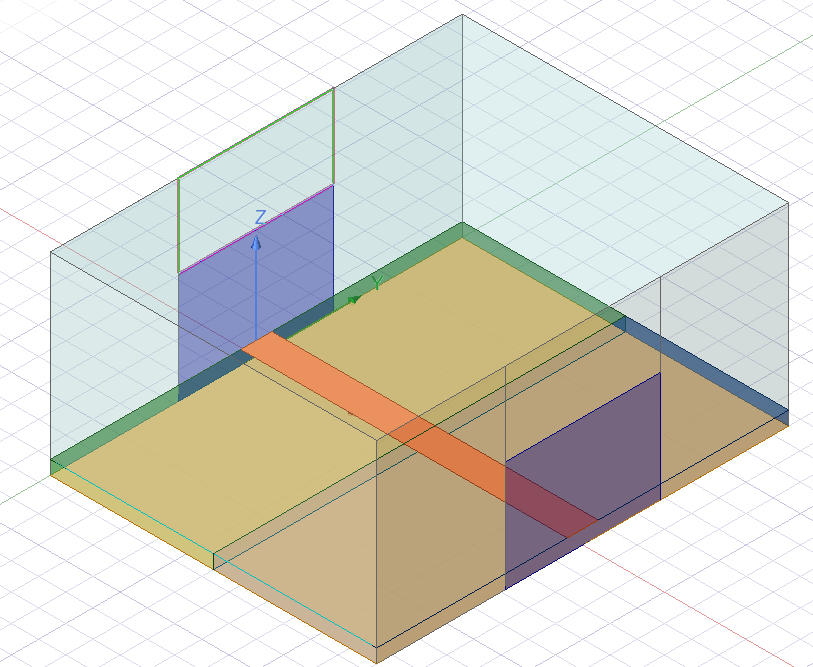
\includegraphics[width=\linewidth]{figuras/hfss3d_d4_sustrato.png}
\caption{Cambio de sustrato}
\end{subfigure}\\[6pt]
\begin{subfigure}[b]{0.32\textwidth}
\centering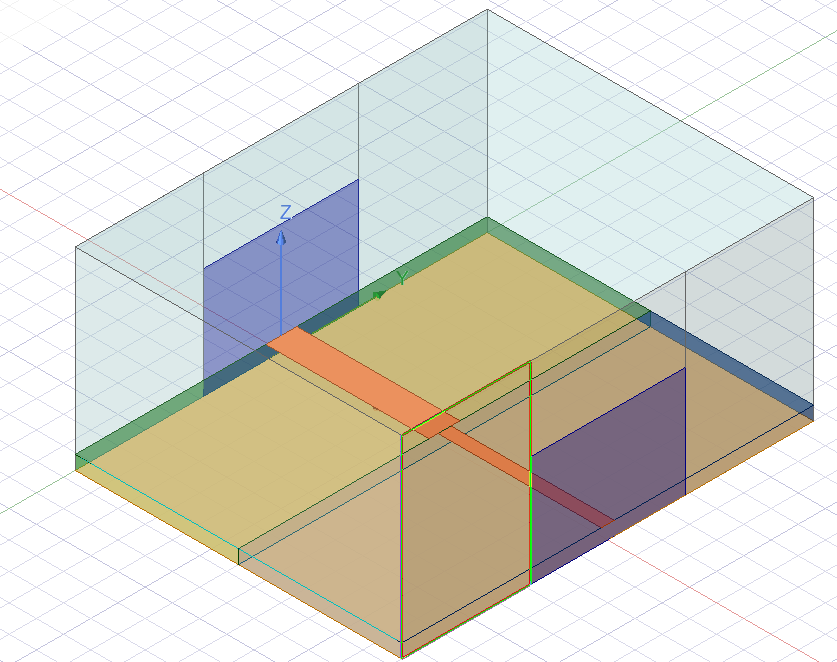
\includegraphics[width=\linewidth]{figuras/hfss3d_d4_compensado.png}
\caption{Sustrato con ancho compensado}
\end{subfigure}\qquad
\begin{subfigure}[b]{0.32\textwidth}
\centering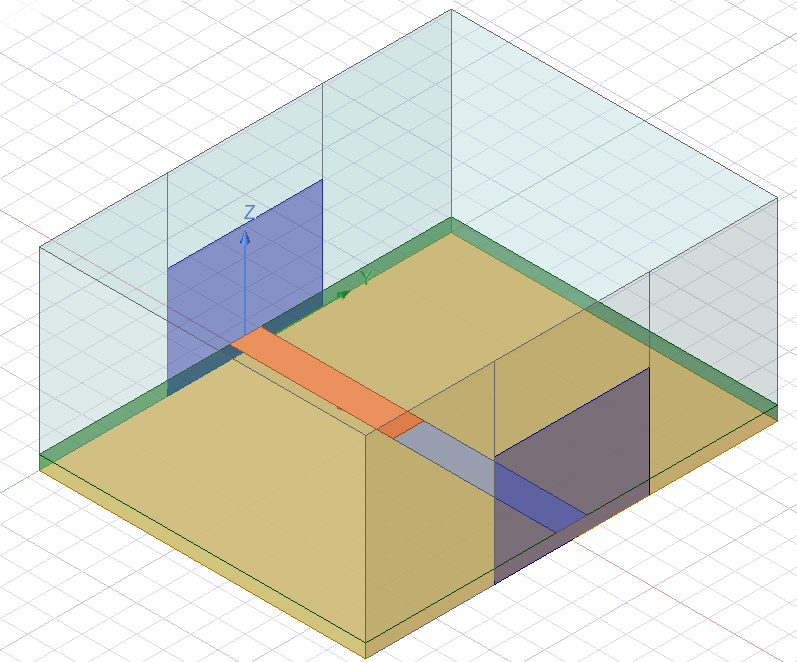
\includegraphics[width=\linewidth]{figuras/hfss3d_d4_estano.png}
\caption{Cambio de metal (estaño en gris)}
\end{subfigure}
\caption{Modelos 3D del cambio de material en HFSS. En (c) y (d) el segundo sustrato aparece en otro tono; las referencias de FR-4, RO3010 y estaño tienen la misma forma que (a).}
\label{fig:d4hfss}
\end{figure}

\paragraph{Tratamiento numérico.} Los parámetros $S$ se corrigieron con \eqref{eq:deembed} (Sección~\ref{sec:correccion}), usando la caja de error de la referencia de cada lado: la de RO4003C en el puerto 1 y la de la línea del segundo material en el puerto 2. El residuo de las referencias corregidas con sus propias cajas es $|S_{11}|\leq <<D4_RESREF4>>$ (\SI{<<D4_RESREF4DB>>}{dB}), que se toma como la resolución de la reflexión. Como referencia ideal se usa el escalón \eqref{eq:gamma0} con las impedancias de los puertos de HFSS, que es lo que reflejaría la unión si no tuviera ningún efecto propio.

\subsection{Resultados}

\subsubsection{Las líneas de cada material}
La Tabla~\ref{tab:d4lineas} reúne los parámetros de las cinco líneas, obtenidos de los puertos de HFSS. Las fórmulas cuasi-estáticas \eqref{eq:eeff} y \eqref{eq:z0} reproducen la impedancia de las cinco líneas con una diferencia menor a \SI{1}{\ohm}. El dato central es que las tres líneas de \SI{1.14}{mm} de cobre tienen la misma inductancia por unidad de longitud (<<D4_LP1>> y <<D4_LP3>>~nH/m sobre RO4003C y RO3010, una diferencia de \SI{<<D4_DLP13>>}{\percent}), mientras que la capacitancia pasa de <<D4_CP1>> a <<D4_CP2>> y a <<D4_CP3>>~pF/m. Esto confirma lo que se esperaba en \eqref{eq:gamman}: cambiar el sustrato solo cambia $C'$. Cambiar el metal no cambia ni $L'$ ni $C'$ (fila del estaño), solo la atenuación.

\begin{table}[htbp]
\centering
\caption{Líneas que intervienen en el cambio de material, a \SI{5}{GHz}: impedancia de las fórmulas cuasi-estáticas y de los puertos de HFSS, permitividad e índice efectivos, inductancia y capacitancia por unidad de longitud y atenuación.}
\label{tab:d4lineas}
\small
\setlength{\tabcolsep}{4pt}
\begin{tabular}{llcccccccc}
\toprule
 & & & \multicolumn{2}{c}{$Z_0$ (\si{\ohm})} & & & & & \\
\cmidrule(lr){4-5}
Sustrato & Metal & $W$ (mm) & \eqref{eq:z0} & HFSS & $\varepsilon_{\mathrm{eff}}$ & $n$ & $L'$ (nH/m) & $C'$ (pF/m) & $\alpha$ (dB/cm) \\
\midrule
<<D4_LINROWS4>>
\bottomrule
\end{tabular}
\end{table}

\subsubsection{Reflexión}
La Figura~\ref{fig:d4refl}a y la Tabla~\ref{tab:d4sparam} muestran la reflexión en la unión. Las dos uniones de sustrato reflejan una cantidad casi constante desde \SI{0.1}{GHz}: $|\Gamma|\approx<<D4_GB1_5>>$ (\SI{<<D4_S11B1_5>>}{dB}, VSWR $=<<D4_VB1_5>>$) al pasar a FR-4 y $|\Gamma|\approx<<D4_GB2_5>>$ (\SI{<<D4_S11B2_5>>}{dB}, VSWR $=<<D4_VB2_5>>$) al pasar a RO3010, lo que equivale a reflejar entre el <<D4_PRB2MIN>> y el <<D4_PRB2MAX>>\,\% de la potencia. Ambas coinciden con el escalón ideal entre las impedancias de los puertos (líneas discontinuas) y con \eqref{eq:gamman}, que con los índices de la Tabla~\ref{tab:d4lineas} da $\Gamma_0=<<D4_GN2_5>>$ y $<<D4_GN3_5>>$. El signo negativo, que se observa en la fase de $S_{11}$ (a menos de \ang{<<D4_ANG11B2MAX>>} de \ang{180} en el caso del RO3010), indica que la onda pasa a una línea de menor impedancia.

\begin{figure}[htbp]
\centering
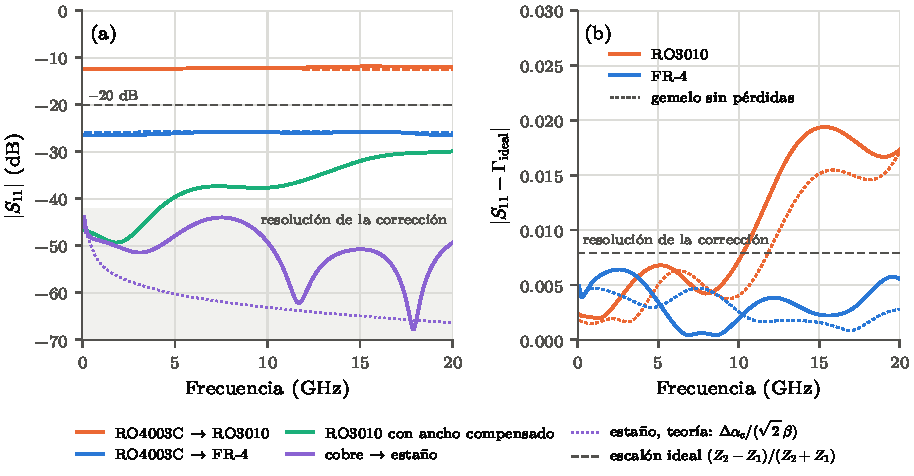
\includegraphics[width=\textwidth]{figuras/fig_d4_reflexion.pdf}
\caption{Cambio de material: (a) reflexión en la unión, con los parámetros corregidos, junto al escalón ideal entre las impedancias de los puertos y a la predicción \eqref{eq:gsn} para el estaño; la zona sombreada está por debajo de la resolución de la corrección. (b) Diferencia entre $S_{11}$ y el escalón ideal en las uniones de sustrato.}
\label{fig:d4refl}
\end{figure}

\begin{table}[htbp]
\centering
\caption{Cambio de material: $|\Gamma|=|S_{11}|$, VSWR y $|S_{21}|$ (dB) en la unión, con parámetros corregidos.}
\label{tab:d4sparam}
\small
\setlength{\tabcolsep}{4pt}
\begin{tabular}{c ccc ccc ccc}
\toprule
 & \multicolumn{3}{c}{RO4003C $\to$ FR-4} & \multicolumn{3}{c}{RO4003C $\to$ RO3010} & \multicolumn{3}{c}{Cobre $\to$ estaño} \\
\cmidrule(lr){2-4}\cmidrule(lr){5-7}\cmidrule(lr){8-10}
$f$ (GHz) & $|\Gamma|$ & VSWR & $S_{21}$ & $|\Gamma|$ & VSWR & $S_{21}$ & $|\Gamma|$ & VSWR & $S_{21}$ \\
\midrule
<<D4_SROWS4>>
\bottomrule
\end{tabular}
\end{table}

La Figura~\ref{fig:d4refl}b muestra cuánto se aparta cada unión del escalón ideal. Hasta \SI{10}{GHz} la diferencia es a lo sumo <<D4_DEVB2_10>>, del orden de la resolución: en ese rango la frontera entre sustratos no agrega ninguna capacitancia ni inductancia apreciable, a diferencia del cambio de ancho. Por encima de \SI{10}{GHz} la unión con RO3010 se aparta hasta <<D4_DEVB2_20>> (su $|S_{11}|$ sube \SI{<<D4_GB2REL>>}{\percent} entre 1 y \SI{20}{GHz}), y lo mismo ocurre en el gemelo sin pérdidas, así que no es un efecto de las pérdidas. Su origen se discute en la Sección~\ref{sec:d4fisica}. La unión con FR-4 no se aparta del escalón ideal en ninguna frecuencia.

El cambio de cobre a estaño no produce una reflexión medible: por encima de \SI{1}{GHz}, $|S_{11}|\leq <<D4_GDMAX_HI>>$, en el nivel de la resolución. La predicción \eqref{eq:gsn}, evaluada con las atenuaciones de HFSS, es de <<D4_GSN1>> a \SI{1}{GHz} y <<D4_GSN20>> a \SI{20}{GHz}, entre <<D4_DBRES1>> y <<D4_DBRES20>>~dB por debajo de lo que la simulación puede resolver.

\subsubsection{Transmisión y potencia}
En las uniones de sustrato, la pérdida de inserción es exactamente la que corresponde a la reflexión: \SI{<<D4_ILB2_5>>}{dB} con RO3010 a \SI{5}{GHz}, igual a $\mathrm{IL}_{\mathrm{refl}}=\SI{<<D4_MLB2_5>>}{dB}$, y \SI{<<D4_ILB1_5>>}{dB} con FR-4. El balance \eqref{eq:balance} de los gemelos sin pérdidas corregidos se mantiene dentro de $\pm\SI{<<D4_BALMAX4>>}{\percent}$ en toda la banda: la unión no radia ni disipa de forma apreciable. La fase de $S_{21}$ tampoco cambia (\ang{<<D4_ANG21B2_20>>} a \SI{20}{GHz} con RO3010), es decir, la frontera no agrega retardo: es una unión de longitud cero. En la unión cobre--estaño, $|S_{21}|$ es \SI{0}{dB} dentro de \SI{<<D4_ILDMAX>>}{dB}, porque el efecto del estaño no está en la unión sino a lo largo de la línea.

\subsubsection{Pérdidas a lo largo de la línea}
La Figura~\ref{fig:d4perd} y la Tabla~\ref{tab:d4alfa} separan la atenuación de las líneas sobre RO4003C. Como el sustrato es el mismo, la pérdida por el dieléctrico \eqref{eq:alfad} es común a las dos líneas, y la diferencia se debe solo al conductor. La tira de estaño aumenta la atenuación total en un <<D4_DA5PCT>>\,\% a \SI{5}{GHz}, y la atenuación por conductor en un factor de <<D4_RATMIN>> a <<D4_RATMAX>>. Si toda la pérdida de conductor estuviera en la tira, el factor sería $\sqrt{\sigma_{\mathrm{Cu}}/\sigma_{\mathrm{Sn}}}=<<D4_RS>>$; como el plano de tierra sigue siendo de cobre, el factor medido indica que la tira produce el <<D4_FRTIRA>>\,\% de la pérdida de conductor, porque la corriente de la tira se concentra en una superficie mucho menor que la del plano de tierra. La atenuación por conductor crece como $f^{<<D4_PCU>>}$, cerca de la ley $\sqrt{f}$ del efecto piel. Para una pista estañada de \SI{10}{cm}, la pérdida adicional va de \SI{<<D4_EXT1>>}{dB} a \SI{1}{GHz} a \SI{<<D4_EXT20>>}{dB} a \SI{20}{GHz}.

\begin{figure}[htbp]
\centering
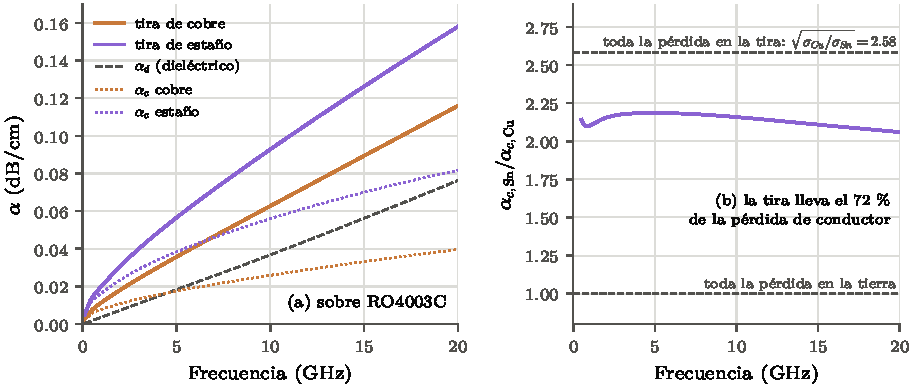
\includegraphics[width=\textwidth]{figuras/fig_d4_perdidas.pdf}
\caption{Pérdidas de la línea sobre RO4003C con tira de cobre y de estaño: (a) atenuación total de los puertos de HFSS, atenuación por el dieléctrico \eqref{eq:alfad} y atenuación por conductor (la diferencia); (b) cociente entre la atenuación por conductor de ambas líneas.}
\label{fig:d4perd}
\end{figure}

\begin{table}[htbp]
\centering
\caption{Atenuación de la línea sobre RO4003C (dB/cm): dieléctrico, conductor con tira de cobre y con tira de estaño, y pérdida adicional de un tramo estañado de \SI{10}{cm}.}
\label{tab:d4alfa}
\small
\begin{tabular}{ccccccc}
\toprule
$f$ (GHz) & $\alpha_d$ & $\alpha_{c,\mathrm{Cu}}$ & $\alpha_{c,\mathrm{Sn}}$ & $\Delta\alpha_c$ & $\alpha_{c,\mathrm{Sn}}/\alpha_{c,\mathrm{Cu}}$ & Adicional en \SI{10}{cm} (dB) \\
\midrule
<<D4_ALFAROWS>>
\bottomrule
\end{tabular}
\end{table}

En el cambio de sustrato ocurre algo parecido con el dieléctrico. La unión con FR-4 casi no refleja, pero el FR-4 tiene un $\tan\delta$ siete veces mayor, y su línea atenúa \SI{<<D4_AFR5>>}{dB/cm} a \SI{5}{GHz}, <<D4_RFR5>> veces más que la de RO4003C (\SI{<<D4_AFR20>>}{dB/cm} a \SI{20}{GHz}). En una línea que pasa a FR-4, la reflexión en la frontera es lo de menos; lo que pesa es la pérdida del tramo que sigue. La línea sobre RO3010, en cambio, atenúa \SI{<<D4_A3_5>>}{dB/cm}, del mismo orden que la de RO4003C.

\subsubsection{Sustrato con ancho compensado}
Con la tira de \SI{0.48}{mm}, la línea sobre RO3010 tiene \SI{<<D4_Z4_5>>}{\ohm} y la reflexión baja de <<D4_GB2_5>> a <<D4_GC_5>> a \SI{5}{GHz}, <<D4_RED>> veces menos (curva verde de la Figura~\ref{fig:d4refl}a). Hasta \SI{2}{GHz} queda en $|S_{11}|\leq <<D4_GCLOW>>$, y en toda la banda en $|S_{11}|\leq <<D4_GCMAX>>$ (\SI{<<D4_S11CMAX>>}{dB}). Lo que queda crece con la frecuencia, porque se debe a los parásitos del cambio de ancho de \SI{1.14}{} a \SI{0.48}{mm}, el mismo mecanismo de la Sección~\ref{sec:d2}: ajustando el circuito de la Figura~\ref{fig:circescalon} se obtiene $C=(<<D4_CCOMP>>\pm<<D4_ECCOMP>>)$~fF y $L_s=(<<D4_LCOMP>>\pm<<D4_ELCOMP>>)$~pH, que retrasan la fase de $S_{21}$ \ang{<<D4_DLY20>>} a \SI{20}{GHz}. La compensación corrige la impedancia, pero no la velocidad: la onda sigue viajando más lento en el RO3010 ($n=<<D4_N4>>$ contra <<D4_N1>>), con $\lambda_g=\SI{<<D4_LG4_5>>}{mm}$ a \SI{5}{GHz} en lugar de \SI{<<D4_LG1_5>>}{mm}, lo que importa para el retardo de la señal, y la tira más angosta atenúa algo más (\SI{<<D4_A4_5>>}{} contra \SI{<<D4_A3_5>>}{dB/cm}).

\subsection{Discusión: explicación física}
\label{sec:d4fisica}

\subsubsection{Por qué el cambio de sustrato refleja}
En la unión, el voltaje y la corriente deben ser continuos, y el campo eléctrico tangente a la frontera entre sustratos también. Bajo la tira ese campo es casi vertical, es decir, tangente a la frontera, así que $\mathbf{E}$ pasa de un sustrato al otro sin cambiar, pero el desplazamiento $\mathbf{D}=\varepsilon\mathbf{E}$ se multiplica por el cociente de permitividades. La Figura~\ref{fig:d4campos}a lo muestra con los campos de HFSS: a través de la unión $|\mathbf{E}|$ cambia en \SI{<<D4_ESALTOPCT>>}{\percent} bajo la tira y \SI{<<D4_EAIREPCT>>}{\percent} en el aire, mientras que $|\mathbf{D}|$ salta un factor de <<D4_DSALTO>> en el sustrato ($10.2/3.55=2.87$). Como la carga de la tira es el $\mathbf{D}$ que termina en ella, la carga por unidad de longitud salta un factor de <<D4_QSALTO>> (Figura~\ref{fig:d4campos}b y c), cercano al cociente de capacitancias de los puertos, <<D4_RCP13>>; el voltaje y la corriente cambian menos de \SI{<<D4_VIMAX>>}{\percent}.

\begin{figure}[htbp]
\centering
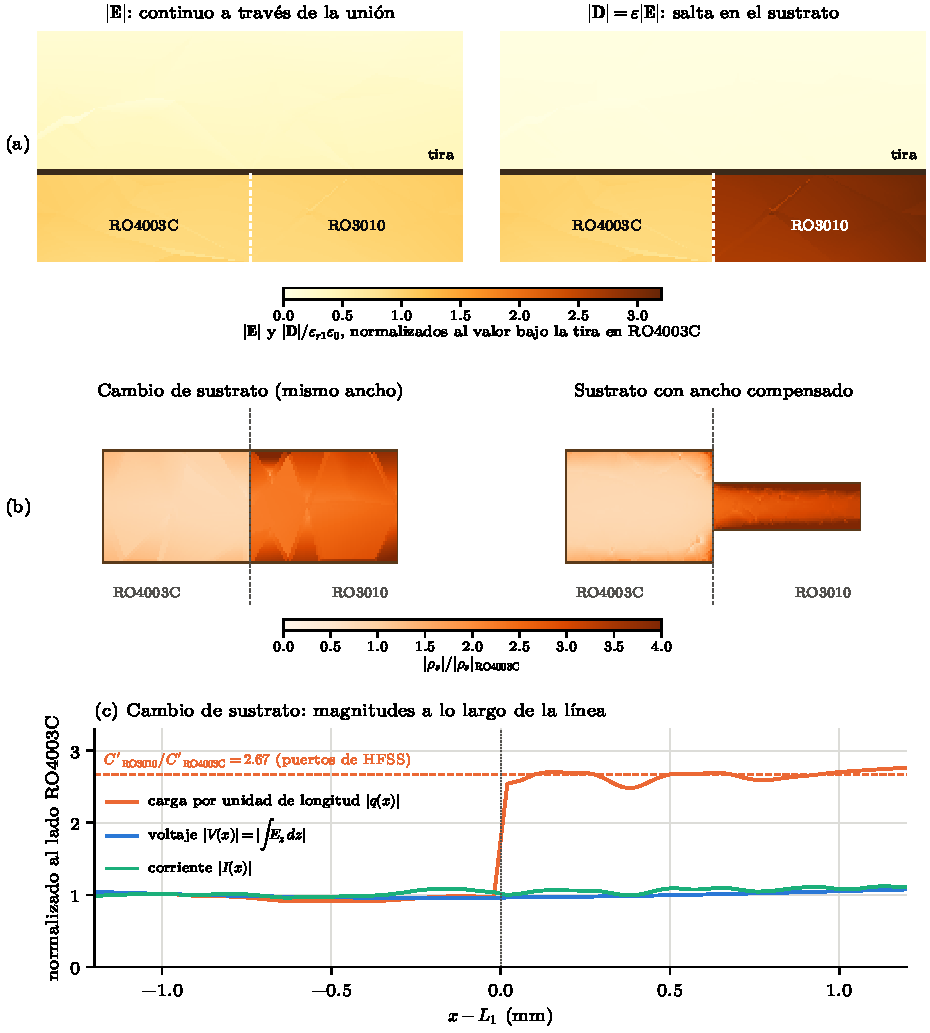
\includegraphics[width=\textwidth]{figuras/fig_d4_campos.pdf}
\caption{Cambio de sustrato a \SI{5}{GHz}, a partir de los campos de HFSS. (a) Magnitud de $\mathbf{E}$ y de $\mathbf{D}$ en el plano vertical que pasa por el eje de la línea, normalizadas a su valor bajo la tira en el RO4003C; la línea punteada es la frontera entre sustratos. (b) Magnitud de la densidad de carga superficial sobre la tira, sin y con el ancho compensado. (c) Carga por unidad de longitud, voltaje (integral de $E_z$ bajo el eje de la tira) y corriente a lo largo de la línea, normalizados a su valor en el RO4003C.}
\label{fig:d4campos}
\end{figure}

El RO3010 necesita entonces <<D4_RCP13>> veces más carga para sostener el mismo voltaje, mientras que el campo magnético, que no depende de $\varepsilon$, y con él la inductancia por unidad de longitud, siguen iguales. Su cociente $V/I=\sqrt{L'/C'}$ es menor, \SI{<<D4_Z3_5>>}{\ohm}. La onda que llega por la línea de \SI{50}{\ohm} no puede entregar en la unión el cociente $V/I$ que exige la línea siguiente, y la diferencia regresa como onda reflejada. Como solo cambia $C'$, el cociente de impedancias es el inverso del cociente de índices efectivos, y la reflexión sigue la misma ley que la de la luz al llegar a un vidrio \eqref{eq:gamman}. El FR-4 refleja poco porque su índice efectivo (<<D4_N2>>) está cerca del de RO4003C (<<D4_N1>>).

Con el ancho compensado, la carga por unidad de longitud también salta (un factor de <<D4_QCSALTO>> en los campos), pero la tira angosta tiene además <<D4_RLP4>> veces más inductancia por unidad de longitud: $L'$ y $C'$ crecen en la misma proporción (<<D4_RLP4>> y <<D4_RCP4>>), su cociente no cambia y no hay reflexión. Lo único que cambia es su producto, que fija la velocidad, y por eso el índice crece en el mismo factor (<<D4_RN4>>).

\paragraph{Por qué no hay parásitos.} En el cambio de ancho la tira cambiaba de forma, y el campo tenía que reorganizarse cerca de la unión: carga de borde en los hombros y corriente concentrada (Sección~\ref{sec:d2}). Aquí la tira no cambia, y la distribución transversal del campo es casi la misma a ambos lados: la fracción del campo que va por el sustrato, el factor de llenado $q=(\varepsilon_{\mathrm{eff}}-1)/(\varepsilon_r-1)$, vale <<D4_Q1>> sobre RO4003C y <<D4_Q3>> sobre RO3010 a \SI{5}{GHz}. Los dos modos cuasi-TEM empalman casi exactamente, y casi no se excitan modos evanescentes que almacenen energía. Por eso la unión es un escalón casi ideal. Con la frecuencia, la dispersión empuja más campo hacia el sustrato de mayor permitividad: $\varepsilon_{\mathrm{eff}}$ del RO3010 pasa de <<D4_EE3_1>> a <<D4_EE3_20>> entre 1 y \SI{20}{GHz}, y la del RO4003C solo de <<D4_EE1_1>> a <<D4_EE1_20>>, de modo que a \SI{20}{GHz} los factores de llenado ya difieren (<<D4_Q1_20>> y <<D4_Q3_20>>). Las distribuciones dejan de coincidir y la reflexión se aparta del escalón ideal en la cantidad que muestra la Figura~\ref{fig:d4refl}b.

\subsubsection{Por qué el cambio de metal casi no refleja}
El metal no interviene en la carga ni en el campo fuera del conductor: $C'$ la fijan la geometría y el dieléctrico, y la inductancia externa la geometría. El metal solo decide qué tan fácil circula la corriente en la delgada capa de su superficie donde se concentra, cuyo espesor es la profundidad de penetración $\delta=\sqrt{2/(\omega\mu_0\sigma)}$: \SI{<<D4_DCU1>>}{\micro\metre} en el cobre y \SI{<<D4_DSN1>>}{\micro\metre} en el estaño a \SI{1}{GHz}. Esa capa agrega una resistencia y una inductancia interna que, por unidad de longitud, son del orden de $2\alpha_c/\beta\sim 10^{-3}$ veces la reactancia de la línea. El cociente $V/I$ cambia apenas, y la reflexión \eqref{eq:gsn} es de milésimas. El efecto del estaño es distribuido: cada centímetro de tira estañada disipa más potencia, y esa pérdida se acumula con la longitud.

\subsubsection{A partir de qué frecuencia el efecto es significativo}
Con el criterio de las otras discontinuidades ($|S_{11}|>-20$~dB), una sola unión entre RO4003C y RO3010 es significativa en toda la banda y desde DC, como el cambio de ancho, porque su reflexión la fija el cociente de impedancias. La unión con FR-4 ($|\Gamma|\approx 0.05$) y la del estaño no lo son en ninguna frecuencia.

Sin embargo, en un interconector real el segundo material ocupa un tramo de longitud $\ell$, después del cual la línea regresa al material original o llega a una carga de \SI{50}{\ohm}. La Figura~\ref{fig:d4tramo} muestra la reflexión a la entrada de un tramo de RO3010 calculada con \eqref{eq:tramo} a partir de los parámetros $S$ de HFSS (la unión, su inversa y la constante de propagación de la línea). A baja frecuencia las reflexiones de las dos uniones, de signo opuesto, se cancelan: un tramo eléctricamente corto de \SI{<<D4_Z3_5>>}{\ohm} es casi invisible. Al subir la frecuencia aparece un desfase entre ellas, y la reflexión supera $-20$~dB cuando el tramo mide $\lambda_g/<<D4_LGF6>>$, independientemente de su longitud (Tabla~\ref{tab:d4tramo}). Llega al máximo de \eqref{eq:tramo}, $2|\Gamma_0|/(1+\Gamma_0^2)\approx<<D4_GPKT>>$, cuando $\ell=\lambda_g/4$, y se anula cada vez que el tramo mide un múltiplo de $\lambda_g/2$. El tramo de FR-4 nunca pasa de <<D4_GPKFR>>, y el compensado de <<D4_GPKC>>.

\begin{figure}[htbp]
\centering
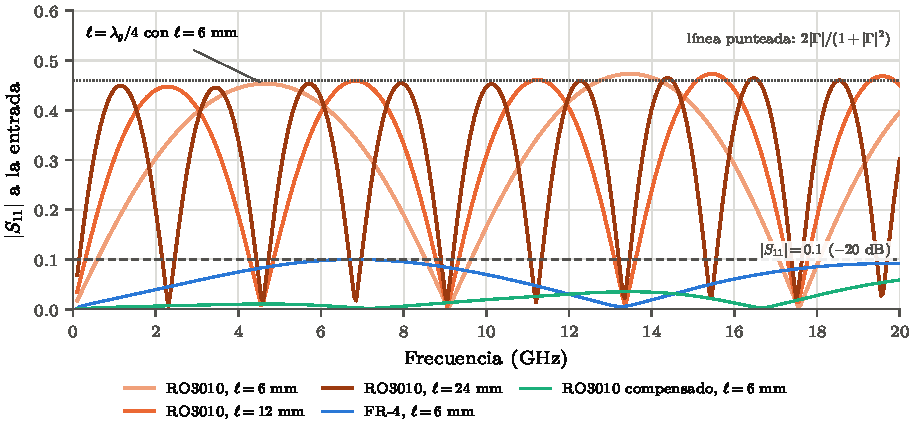
\includegraphics[width=\textwidth]{figuras/fig_d4_tramo.pdf}
\caption{Reflexión a la entrada de un tramo de longitud $\ell$ del segundo material entre dos líneas de RO4003C (o terminado en \SI{50}{\ohm}), calculada con la unión corregida de HFSS, su inversa y la constante de propagación de la línea del segundo material.}
\label{fig:d4tramo}
\end{figure}

\begin{table}[htbp]
\centering
\caption{Tramo de RO3010 de longitud $\ell$: frecuencia a la que la reflexión supera $-20$~dB, frecuencia a la que el tramo mide $\lambda_g/4$, longitud eléctrica del tramo en el cruce y reflexión máxima hasta \SI{20}{GHz}.}
\label{tab:d4tramo}
\small
\begin{tabular}{ccccc}
\toprule
$\ell$ (mm) & $|S_{11}|>-20$~dB desde (GHz) & $\ell=\lambda_g/4$ (GHz) & $\ell$ en el cruce & $|S_{11}|$ máx. \\
\midrule
<<D4_FINROWS>>
\bottomrule
\end{tabular}
\end{table}

Así, el efecto del cambio de sustrato depende de la frecuencia solo a través de la longitud eléctrica del tramo, y la frecuencia a partir de la cual es significativo es inversamente proporcional a $\ell$: \SI{<<D4_FS6>>}{GHz} para \SI{6}{mm}, \SI{<<D4_FS12>>}{GHz} para \SI{12}{mm} y \SI{<<D4_FS24>>}{GHz} para \SI{24}{mm}. El cambio de metal no tiene un umbral en frecuencia: su pérdida adicional crece como $\sqrt{f}$ y en proporción a la longitud del tramo estañado (Tabla~\ref{tab:d4alfa}).

%======================================================================
\section{Discontinuidad 5: unión en T}
\label{sec:d5}

\subsection{Diseño y estructuras simuladas}
Se simularon tres versiones de la misma unión, con la rama perpendicular a la línea principal (Figura~\ref{fig:d5geo}):
\begin{itemize}
\item \textbf{T de \SI{50}{\ohm}.} Los tres brazos son líneas de \SI{50}{\ohm} de \SI{1.14}{mm} y cada uno termina en un puerto: P1 y P2 en los extremos de la línea principal y P3 en la rama. Es el caso de un interconector con una derivación.
\item \textbf{Divisor en T.} La rama de \SI{50}{\ohm} es la entrada (P3) y la línea principal es de \SI{100}{\ohm} (\SI{0.29}{mm}, la misma línea de la discontinuidad 2), de modo que $100\parallel 100=\SI{50}{\ohm}$. Es la versión corregida de la T: sin diferencia de impedancias en la entrada, lo que quede de reflexión se debe solo a la unión.
\item \textbf{Stub abierto.} La misma T de \SI{50}{\ohm}, pero la rama mide \SI{8}{mm} y termina en circuito abierto, sin puerto: una derivación que no lleva a ninguna parte.
\end{itemize}
Tras el de-embedding de $L_1$, los planos de referencia quedan en los bordes del cuadro de unión: los de la línea principal en los bordes de la rama y el de la rama en el borde de la línea principal, igual que en el modelo de Hammerstad. Se agregaron las líneas de referencia de \SI{50}{\ohm} y \SI{100}{\ohm} y el gemelo sin pérdidas de cada estructura, en total <<D5_NDIS5>> diseños (Figura~\ref{fig:d5hfss}).

\begin{figure}[htbp]
\centering
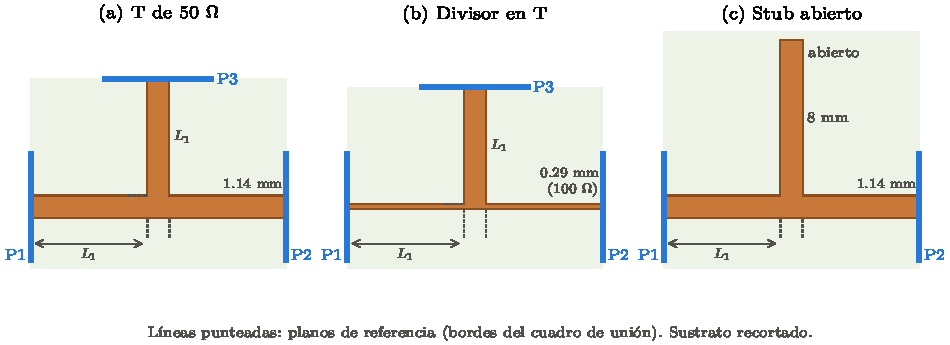
\includegraphics[width=\textwidth]{figuras/fig_d5_geometria.pdf}
\caption{Unión en T: las tres estructuras simuladas, con los puertos y los planos de referencia.}
\label{fig:d5geo}
\end{figure}

\begin{figure}[htbp]
\centering
\begin{subfigure}[b]{0.32\textwidth}
\centering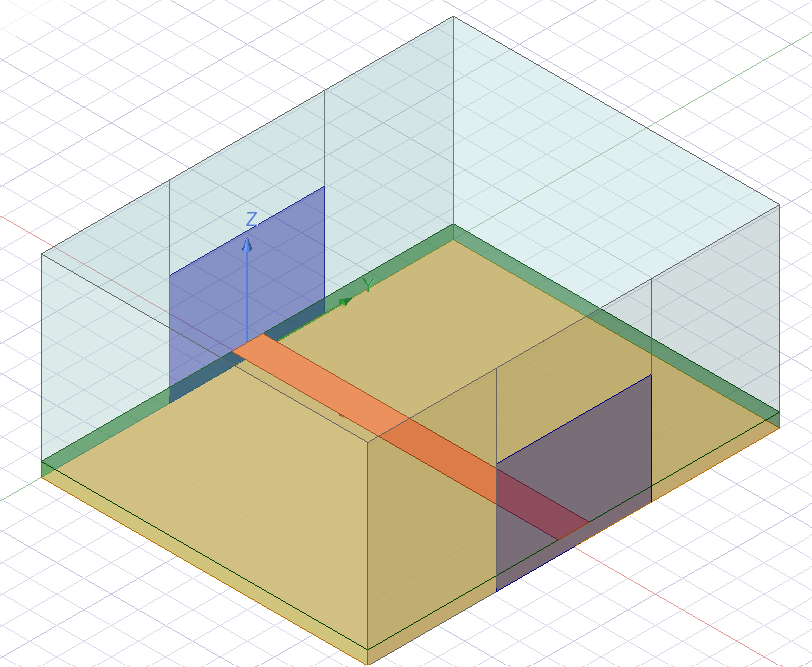
\includegraphics[width=\linewidth]{figuras/hfss3d_d5_ref50.png}
\caption{Referencia de \SI{50}{\ohm}}
\end{subfigure}\hfill
\begin{subfigure}[b]{0.32\textwidth}
\centering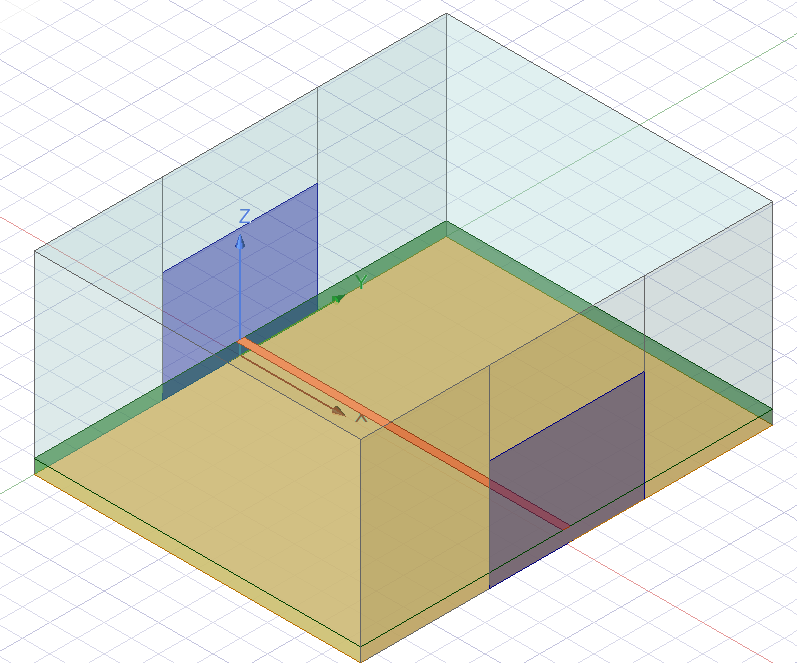
\includegraphics[width=\linewidth]{figuras/hfss3d_d5_ref100.png}
\caption{Referencia de \SI{100}{\ohm}}
\end{subfigure}\hfill
\begin{subfigure}[b]{0.32\textwidth}
\centering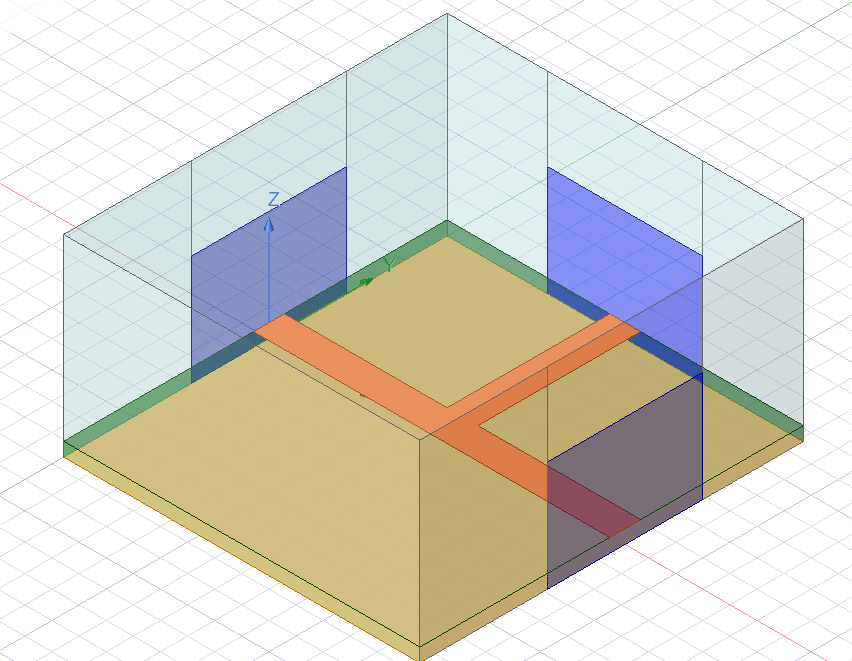
\includegraphics[width=\linewidth]{figuras/hfss3d_d5_T.png}
\caption{T de \SI{50}{\ohm}}
\end{subfigure}\\[6pt]
\begin{subfigure}[b]{0.32\textwidth}
\centering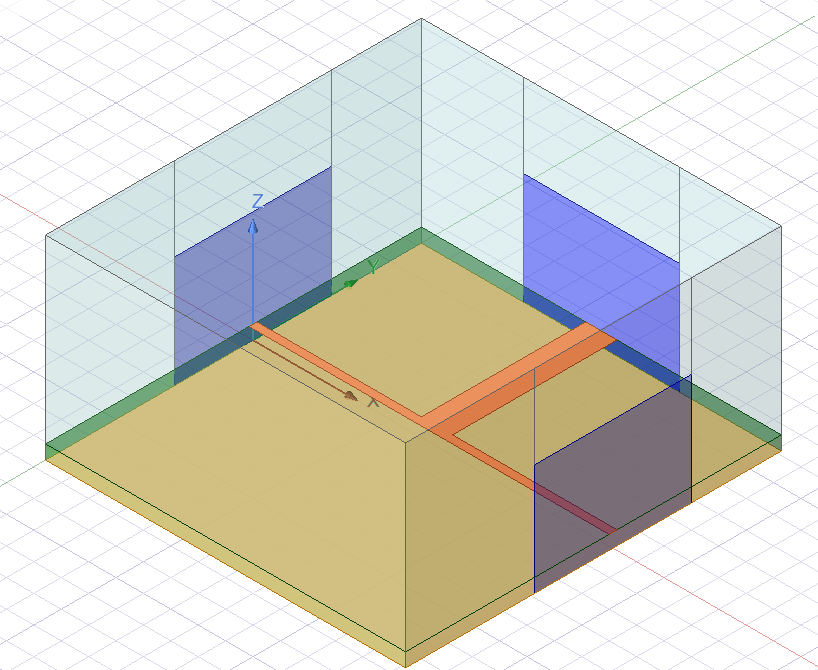
\includegraphics[width=\linewidth]{figuras/hfss3d_d5_divisor.png}
\caption{Divisor en T}
\end{subfigure}\qquad
\begin{subfigure}[b]{0.32\textwidth}
\centering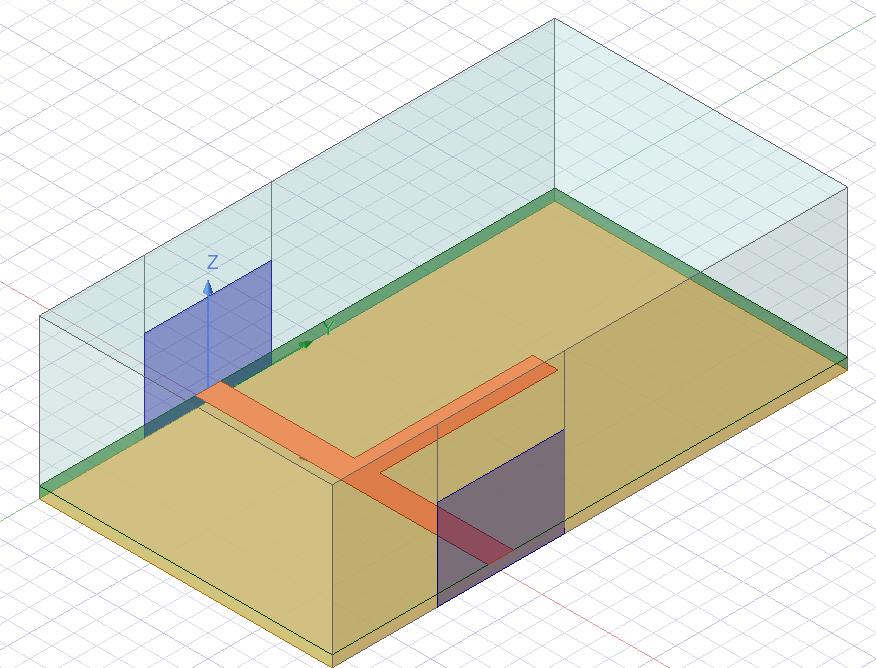
\includegraphics[width=\linewidth]{figuras/hfss3d_d5_stub.png}
\caption{Stub abierto}
\end{subfigure}
\caption{Modelos 3D de la unión en T en HFSS. El tercer puerto de la T y del divisor está en la cara de la caja por la que sale la rama.}
\label{fig:d5hfss}
\end{figure}

\paragraph{Tratamiento numérico.} Con tres puertos, la corrección \eqref{eq:deembed} se generaliza con una caja de error por puerto. Si $\mathbf{D}_{00}$, $\mathbf{D}_{01}$ y $\mathbf{D}_{11}$ son las matrices diagonales con la reflexión externa, la transmisión y la reflexión interna de cada caja,
\begin{gather}
\mathbf{S}_m = \mathbf{D}_{00}+\mathbf{D}_{01}\,\mathbf{S}\left(\mathbf{I}-\mathbf{D}_{11}\mathbf{S}\right)^{-1}\mathbf{D}_{01}
\quad\Longrightarrow \nonumber\\[3pt]
\mathbf{S} = \left(\mathbf{I}+\mathbf{X}\mathbf{D}_{11}\right)^{-1}\mathbf{X},\qquad \mathbf{X}=\mathbf{D}_{01}^{-1}\left(\mathbf{S}_m-\mathbf{D}_{00}\right)\mathbf{D}_{01}^{-1}.
\label{eq:deembedn}
\end{gather}
Con dos puertos esta expresión da exactamente lo mismo que \eqref{eq:deembed} (la diferencia es del orden de $10^{-14}$). Los puertos de \SI{50}{\ohm} se corrigieron con la referencia de \SI{50}{\ohm} y los del divisor de \SI{100}{\ohm} con la de \SI{100}{\ohm}; el residuo de las referencias corregidas es $|S_{11}|\leq <<D5_RESREF5>>$.

\subsection{Resultados}

\subsubsection{La T de \SI{50}{\ohm}}
A baja frecuencia la T se comporta exactamente como la unión ideal \eqref{eq:tideal} (Tabla~\ref{tab:d5sparam} y Figura~\ref{fig:d5t}): a \SI{0.1}{GHz}, $|S_{11}|=<<D5_B11_01>>$ (\SI{<<D5_S11B_01DB>>}{dB}, VSWR $=<<D5_VB1_01>>$), $|S_{21}|=<<D5_B21_01>>$ y $|S_{31}|=<<D5_B31_01>>$, es decir, se refleja el <<D5_PR11_01>>\,\% de la potencia y cada brazo recibe el <<D5_PT21_01>>\,\%. La reflexión de un tercio está presente desde DC y no la causa ningún parásito: es la división de impedancias.

Al subir la frecuencia el reparto deja de ser simétrico. Desde P1, $|S_{11}|$ baja a <<D5_B11_20>> a \SI{20}{GHz}, la potencia que sigue de frente sube al <<D5_PT21_20>>\,\% y la que entra a la rama baja al <<D5_PT31_20>>\,\%. El desbalance $|S_{21}|/|S_{31}|$ supera \SI{0.5}{dB} a partir de \SI{<<D5_FDESB05>>}{GHz} y \SI{1}{dB} a partir de \SI{<<D5_FDESB1>>}{GHz}, y llega a \SI{<<D5_DESB20>>}{dB} a \SI{20}{GHz}. Desde la rama ocurre lo contrario: $|S_{33}|$ crece de <<D5_B33_01>> a <<D5_B33_20>> (VSWR $=<<D5_VB3_20>>$). Las fases también difieren: a \SI{20}{GHz} la transmisión de frente se retrasa \ang{<<D5_ANG21_20>>}, casi lo que tarda la onda en cruzar el cuadro de \SI{1.14}{mm} (\ang{-<<D5_FASEW20>>}), y la que entra a la rama solo \ang{<<D5_ANG31_20>>}.

\begin{table}[htbp]
\centering
\caption{T de \SI{50}{\ohm}: reflexión desde la línea principal (P1) y desde la rama (P3), transmisión a cada brazo y desbalance entre ellos.}
\label{tab:d5sparam}
\small
\begin{tabular}{cccccccc}
\toprule
$f$ (GHz) & $|S_{11}|$ & VSWR$_1$ & $|S_{21}|$ & $|S_{31}|$ & $|S_{21}|/|S_{31}|$ (dB) & $|S_{33}|$ & VSWR$_3$ \\
\midrule
<<D5_SROWS5>>
\bottomrule
\end{tabular}
\end{table}

\begin{figure}[htbp]
\centering
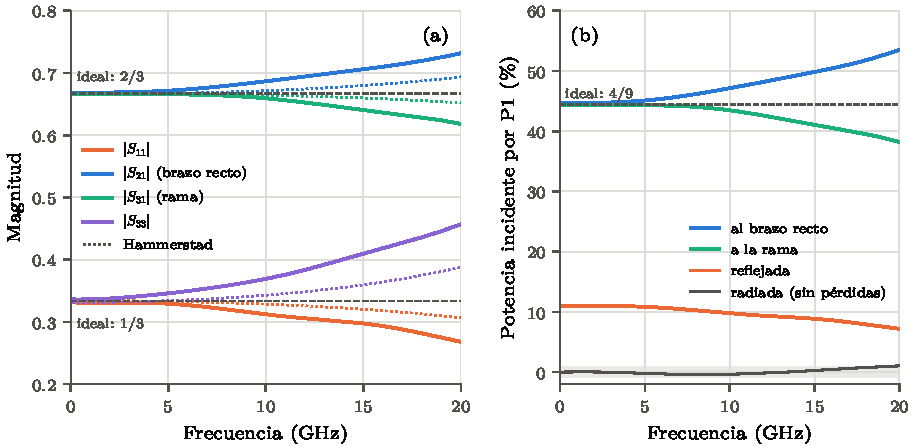
\includegraphics[width=\textwidth]{figuras/fig_d5_T.pdf}
\caption{T de \SI{50}{\ohm}: (a) magnitud de los parámetros $S$ corregidos, frente a la unión ideal \eqref{eq:tideal} y al modelo de Hammerstad \eqref{eq:hammerstad}; (b) destino de la potencia que entra por la línea principal, con la radiación de los gemelos sin pérdidas y su banda de incertidumbre.}
\label{fig:d5t}
\end{figure}

\paragraph{Comparación con el modelo de Hammerstad.} El modelo \eqref{eq:hammerstad}, evaluado con las impedancias y permitividades efectivas de los puertos de HFSS, reproduce la fase de los cuatro parámetros con una diferencia máxima de \ang{<<D5_HFASEMAX>>} hasta \SI{20}{GHz} (a esa frecuencia predice \ang{<<D5_HFASE21_20>>} para $S_{21}$) y la tendencia de las magnitudes, pero subestima su variación: predice un desbalance de \SI{<<D5_HDESB20>>}{dB} a \SI{20}{GHz} en lugar de \SI{<<D5_DESB20>>}{dB}, y $|S_{33}|=<<D5_H33_20>>$ en lugar de <<D5_B33_20>>. Es decir, acierta en dónde están los planos efectivos de la unión, pero le asigna menos energía almacenada de la que encuentra HFSS.

\paragraph{Capacitancia en exceso.} Una forma directa de medir esa energía es comparar la admitancia que se ve desde la rama con la de las dos líneas principales en paralelo. La diferencia es una susceptancia, $\omega C_{\mathrm{ex}}=\mathrm{Im}\{Y_{\mathrm{ent},3}\}-\mathrm{Im}\{1/Z_1+1/Z_2\}$ (Figura~\ref{fig:d5div}b). Entre 2 y \SI{5}{GHz} la T se comporta como una capacitancia en paralelo de $C_{\mathrm{ex}}=(<<D5_CE_B_T>>\pm<<D5_ECE_B_T>>)$~fF, el <<D5_RCW>> de la capacitancia de un tramo de línea de \SI{50}{\ohm} de longitud $W$ ($C'W=\SI{<<D5_CW>>}{fF}$); el modelo de Hammerstad da \SI{<<D5_HCE_B_T>>}{fF}. Por encima de unos \SI{5}{GHz} el valor efectivo baja (\SI{<<D5_CE_B_T10>>}{fF} a \SI{10}{GHz}), porque la inductancia de los caminos de corriente a través del cuadro empieza a compensarla.

\subsubsection{Divisor en T}
El divisor resuelve la reflexión de la T: a baja frecuencia la entrada por la rama refleja $|S_{33}|=<<D5_D33_1>>$ a \SI{1}{GHz}, contra un tercio de la T de \SI{50}{\ohm} (Tabla~\ref{tab:d5div} y Figura~\ref{fig:d5div}a). Lo que queda crece con la frecuencia: <<D5_D33_5>> a \SI{5}{GHz}, <<D5_D33_10>> a \SI{10}{GHz} y <<D5_D33_20>> (\SI{<<D5_D33_20DB>>}{dB}) a \SI{20}{GHz}, y supera $-20$~dB a partir de \SI{<<D5_FD20>>}{GHz}. Su fase es de unos \ang{<<D5_DANG33>>}, es decir, la unión es capacitiva, y la capacitancia en exceso es prácticamente constante: $C_{\mathrm{ex}}=(<<D5_CE_C_Divisor>>\pm<<D5_ECE_C_Divisor>>)$~fF entre 2 y \SI{15}{GHz} (Hammerstad: \SI{<<D5_HCE_C_Divisor>>}{fF}). La potencia se reparte por igual: $|S_{13}|=|S_{23}|=<<D5_D13_5>>$ (\SI{<<D5_D13_5DB>>}{dB}) a \SI{5}{GHz} y \SI{<<D5_D13_20DB>>}{dB} a \SI{20}{GHz}, con un desbalance de solo \SI{<<D5_DDESB20>>}{dB}, porque la estructura es simétrica respecto a la rama. Como predice la teoría, las salidas no quedan acopladas ni aisladas: $|S_{11}|=<<D5_D11_5>>$ y $|S_{12}|=<<D5_D12_5>>$.

\begin{table}[htbp]
\centering
\caption{Divisor en T: reflexión en la entrada (rama, P3), transmisión a una salida y reflexión y acoplamiento entre las salidas.}
\label{tab:d5div}
\small
\begin{tabular}{cccccccc}
\toprule
$f$ (GHz) & $|S_{33}|$ & VSWR$_3$ & $|S_{33}|$ (dB) & $|S_{13}|$ & $|S_{13}|$ (dB) & $|S_{11}|$ & $|S_{12}|$ \\
\midrule
<<D5_DROWS5>>
\bottomrule
\end{tabular}
\end{table}

\begin{figure}[htbp]
\centering
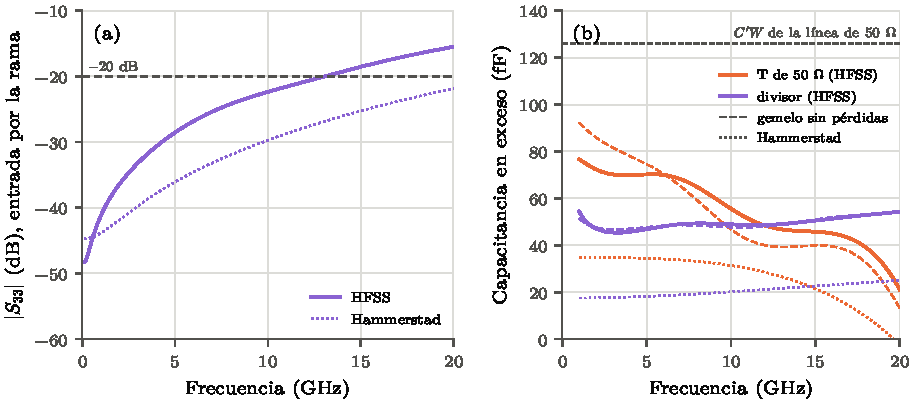
\includegraphics[width=\textwidth]{figuras/fig_d5_divisor.pdf}
\caption{(a) Reflexión en la entrada del divisor, frente al modelo de Hammerstad (la unión ideal da $|S_{33}|<-44$~dB con las impedancias de los puertos). (b) Capacitancia en exceso vista desde la rama en la T de \SI{50}{\ohm} y en el divisor.}
\label{fig:d5div}
\end{figure}

\subsubsection{Potencia}
La Tabla~\ref{tab:d5pot} resume el destino de la potencia. La disipación en la unión es despreciable (a lo sumo \SI{0.1}{\percent}), y la radiación es pequeña: desde la línea principal, \SI{<<D5_PRADB1_20>>}{\percent} a \SI{20}{GHz}; desde la rama, \SI{<<D5_PRADB3_20>>}{\percent} en la T y \SI{<<D5_PRADC3_20>>}{\percent} en el divisor. La incertidumbre, tomada como el valor negativo más grande por debajo de \SI{8}{GHz}, es de $\pm\SI{<<D5_PISO5>>}{\percent}$.

\begin{table}[htbp]
\centering
\caption{Unión en T: destino de la potencia incidente (\%), con parámetros corregidos.}
\label{tab:d5pot}
\small
\begin{tabular}{lcccccc}
\toprule
Excitación & $f$ (GHz) & Reflejada & Salida 1 & Salida 2 & Radiada & Disipada \\
\midrule
<<D5_POWROWS5>>
\bottomrule
\multicolumn{7}{l}{\footnotesize Salidas: P2 y P3 desde P1; P1 y P2 desde P3.}
\end{tabular}
\end{table}

\subsubsection{Stub abierto}
Con la rama abierta, la línea principal deja de transmitir en dos bandas (Figura~\ref{fig:d5stub}a): $|S_{21}|$ cae a \SI{<<D5_DN1>>}{dB} a \SI{<<D5_FN1>>}{GHz} y a \SI{<<D5_DN2>>}{dB} a \SI{<<D5_FN2>>}{GHz}, frecuencias cuyo cociente es <<D5_RN21>>, cerca del 3 que predice \eqref{eq:stub} (la dispersión lo reduce un poco). En la primera, la transmisión está por debajo de $-10$~dB entre \SI{<<D5_BW10A>>}{} y \SI{<<D5_BW10B>>}{GHz} y por debajo de $-3$~dB entre \SI{<<D5_BW3A>>}{} y \SI{<<D5_BW3B>>}{GHz}, y la reflexión es casi total ($|S_{11}|=<<D5_G11N1>>$). A esa frecuencia $\lambda_g=\SI{<<D5_LGQ>>}{mm}$, de modo que el stub, alargado \SI{<<D5_DL3>>}{mm} por su extremo abierto, mide un cuarto de onda; con esa longitud efectiva \eqref{eq:stub} predice \SI{<<D5_FQ>>}{GHz}.

El stub también se puede predecir sin simularlo, combinando resultados ya obtenidos: los parámetros $S$ de tres puertos de la T de \SI{50}{\ohm}, un tramo de \SI{8}{mm} de la línea de referencia y la reflexión del extremo abierto medida en la discontinuidad 3 (el gap de \SI{3}{mm}). Terminando el puerto 3 de la T con $\Gamma_L=\Gamma_{\mathrm{oc}}\,e^{-2\gamma\ell}$,
\begin{equation}
S_{ij}^{\mathrm{stub}} = S_{ij}+\frac{S_{i3}\,\Gamma_L\,S_{3j}}{1-S_{33}\Gamma_L},\qquad i,j\in\{1,2\},
\label{eq:stubpred}
\end{equation}
se obtienen los mínimos en \SI{<<D5_FP1>>}{} y \SI{<<D5_FP2>>}{GHz}, a \SI{<<D5_EFP1>>}{\percent} y \SI{<<D5_EFP2>>}{\percent} de los de HFSS (líneas discontinuas de la Figura~\ref{fig:d5stub}a). Con la extensión de Hammerstad para el extremo abierto (\SI{<<D5_DLHAM>>}{mm}) en lugar de la medida, el resultado es prácticamente el mismo (\SI{<<D5_FPH1>>}{} y \SI{<<D5_FPH2>>}{GHz}). El stub es la estructura que más radia de esta discontinuidad (Figura~\ref{fig:d5stub}b): poco en la primera resonancia (\SI{<<D5_PRADD_N1>>}{\percent}), pero hasta \SI{<<D5_PRADD_MAX>>}{\percent} cerca de la segunda, a \SI{<<D5_FRADD_MAX>>}{GHz}.

\begin{figure}[htbp]
\centering
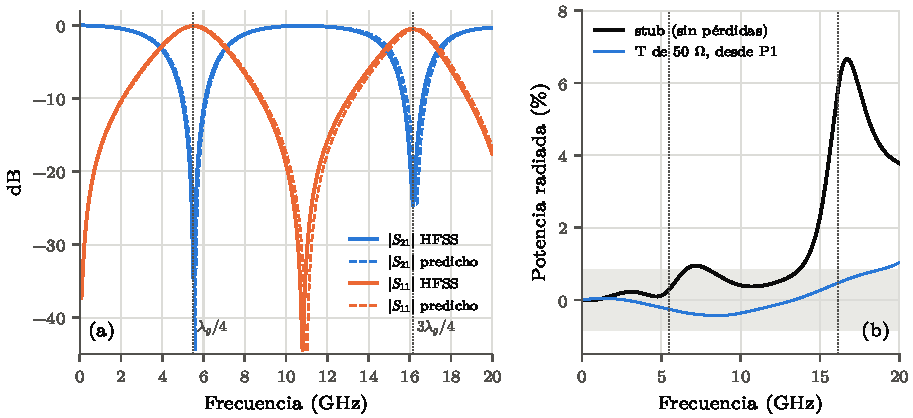
\includegraphics[width=\textwidth]{figuras/fig_d5_stub.pdf}
\caption{Stub abierto de \SI{8}{mm}: (a) transmisión y reflexión de HFSS, frente a la predicción \eqref{eq:stubpred} con la T de tres puertos, la línea de referencia y el extremo abierto de la discontinuidad 3; (b) potencia radiada (gemelos sin pérdidas, corregidos), comparada con la de la T de \SI{50}{\ohm}.}
\label{fig:d5stub}
\end{figure}

\subsection{Discusión: explicación física}
\label{sec:d5fisica}

\subsubsection{Por qué la T refleja un tercio}
En la unión las tres líneas comparten el mismo voltaje, y la corriente que llega se tiene que repartir entre las otras dos. Cada una de ellas exige el cociente $V/I$ de \SI{50}{\ohm}, así que juntas piden el doble de corriente para el mismo voltaje: se comportan como \SI{25}{\ohm}. La onda que llega no puede entregar ese cociente y la diferencia regresa como una onda reflejada de $-1/3$. Es el mismo mecanismo del cambio de ancho y del cambio de sustrato: una diferencia de impedancias que no depende de la frecuencia. La Figura~\ref{fig:d5campos}a lo muestra con los campos de HFSS a \SI{5}{GHz}: la corriente que llega por la izquierda se divide en dos partes iguales; a \SI{1.2}{mm} de la unión, la del brazo recto y la de la rama valen <<D5_IDER>> y <<D5_IRAMA>> veces la del brazo de entrada.

\begin{figure}[htbp]
\centering
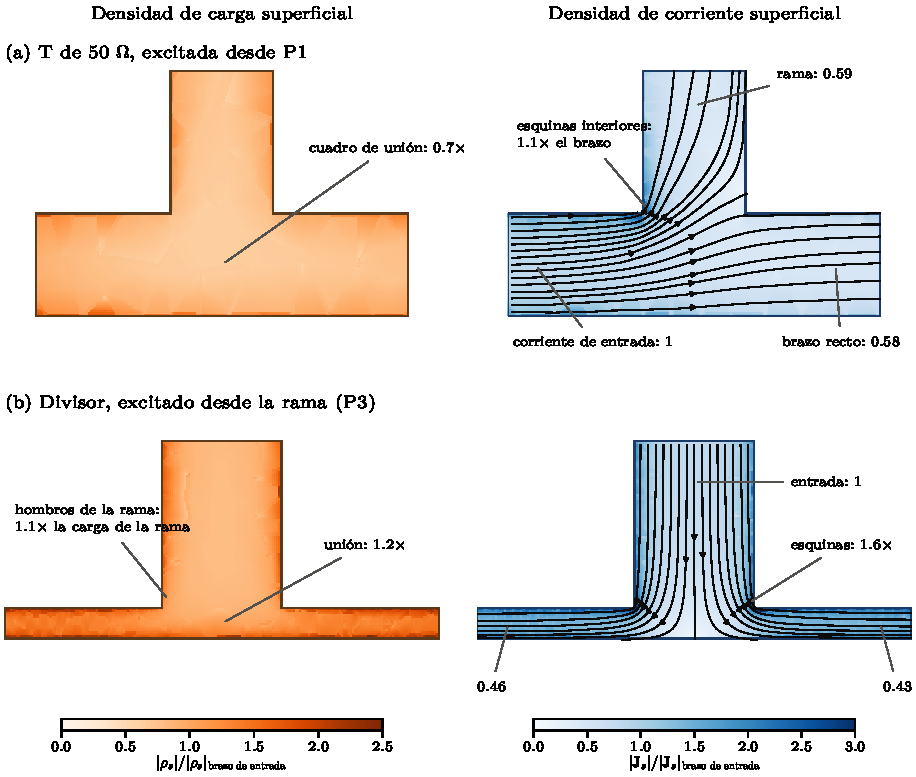
\includegraphics[width=\textwidth]{figuras/fig_d5_campos.pdf}
\caption{Unión en T a \SI{5}{GHz}, a partir de los campos de HFSS: magnitud de la densidad de carga y de la densidad de corriente superficiales, con las líneas de flujo de la corriente, normalizadas a su valor en el brazo de entrada. (a) T de \SI{50}{\ohm} excitada desde P1; (b) divisor excitado desde la rama. Los números del panel de corriente son las corrientes totales de cada brazo, a \SI{1.2}{mm} de la unión, respecto a la del brazo de entrada.}
\label{fig:d5campos}
\end{figure}

\subsubsection{Por qué el reparto cambia con la frecuencia}
Los parásitos de la T vienen de dos lugares. El primero es el cuadro de metal donde se cruzan las líneas. No pertenece a ninguna de ellas y tiene campo de borde solo en un lado, el opuesto a la rama; los otros tres continúan en metal. Su densidad de carga es <<D5_CCUADRO>> veces la de la línea (Figura~\ref{fig:d5campos}a), y por eso su capacitancia es una fracción de la de un tramo recto de la misma longitud, los \SI{<<D5_CE_B_T>>}{fF} medidos. Esa capacitancia está en el nodo y la ven los tres puertos. El segundo es el giro de la corriente: para entrar a la rama, la corriente de la mitad superior de la línea tiene que doblar \ang{90} y se concentra en las esquinas interiores (<<D5_JESQ>> veces la densidad del brazo), como en la curva de la discontinuidad 1, mientras que la de la mitad inferior sigue de frente. El camino hacia la rama tiene así más inductancia que el camino recto. Como la reactancia de esa inductancia crece con $\omega$, la rama acepta cada vez menos corriente, y la potencia que sobra sigue de frente: de ahí que $|S_{21}|$ crezca, $|S_{31}|$ baje y, desde la rama, $|S_{33}|$ aumente. Ambos efectos son de energía almacenada, no de pérdidas: el balance de los gemelos sin pérdidas muestra que la unión no radia más de unos pocos por ciento.

\subsubsection{Por qué el divisor refleja a alta frecuencia}
En el divisor la entrada está acoplada en impedancia, y la reflexión que queda la produce solo la unión. Aquí la rama de \SI{1.14}{mm} desemboca en una línea de \SI{0.29}{mm}, y entre los planos de referencia queda, bajo la boca de la rama, un tramo de \SI{1.14}{mm} de la línea principal que no pertenece a ninguna de las líneas conectadas. Ahí la densidad de carga es <<D5_CCUADROC>> veces la de la rama (Figura~\ref{fig:d5campos}b), y la corriente de la rama se concentra al doblar hacia la línea angosta (<<D5_JESQC>> veces en las esquinas). El resultado neto es la capacitancia en paralelo de \SI{<<D5_CE_C_Divisor>>}{fF}, del orden de la de ese tramo de línea de \SI{100}{\ohm} ($C'W=\SI{<<D5_CW100>>}{fF}$), cuya reflexión, $|S_{33}|\approx\omega C_{\mathrm{ex}}Z_0/2$, crece en proporción a la frecuencia. Para reducirla habría que reducir ese metal, por ejemplo afinando la rama antes de la unión, de la misma manera que el chaflán reduce el de la curva.

\subsubsection{Por qué el stub corta la transmisión}
El extremo abierto refleja la onda con $\Gamma\approx+1$. Cuando el stub mide un cuarto de onda, la onda que vuelve a la unión ha recorrido media longitud de onda: llega invertida y cancela al voltaje que había ahí. La rama pone entonces un corto en la línea principal, y la onda que llega por P1 se refleja casi por completo. En $3\lambda_g/4$ ocurre lo mismo, y entre ambas resonancias el stub tiene una longitud de media onda, en la que su admitancia vuelve a ser nula y la línea transmite casi como si no existiera. A baja frecuencia el stub es una capacitancia de $C'\ell_{\mathrm{ef}}=\SI{<<D5_CSTUB>>}{pF}$ en paralelo, mucho mayor que la del cuadro de unión.

Los campos de HFSS muestran este mecanismo directamente (Figura~\ref{fig:d5stubmapas}). A \SI{5.5}{GHz} la carga se acumula en el extremo abierto y casi desaparece en la unión, y la corriente que llega por el brazo de entrada dobla completa hacia el stub: la que sigue por la línea principal después de la unión es el <<D5S_IOUTA>>\,\% de la que llega. A \SI{10.8}{GHz} la unión tiene la misma carga que la línea, el mínimo de carga queda a la mitad del stub y la corriente sigue de frente (después de la unión es <<D5S_IOUTB>> veces la de antes). A \SI{16.15}{GHz} se repite el corte: la corriente vuelve a entrar al stub, pero solo hasta un nodo a \SI{<<D5S_SIMINC>>}{mm} de la unión, donde cambia de sentido, y la que sigue por la línea es el <<D5S_IOUTC>>\,\%.

\begin{figure}[htbp]
\centering
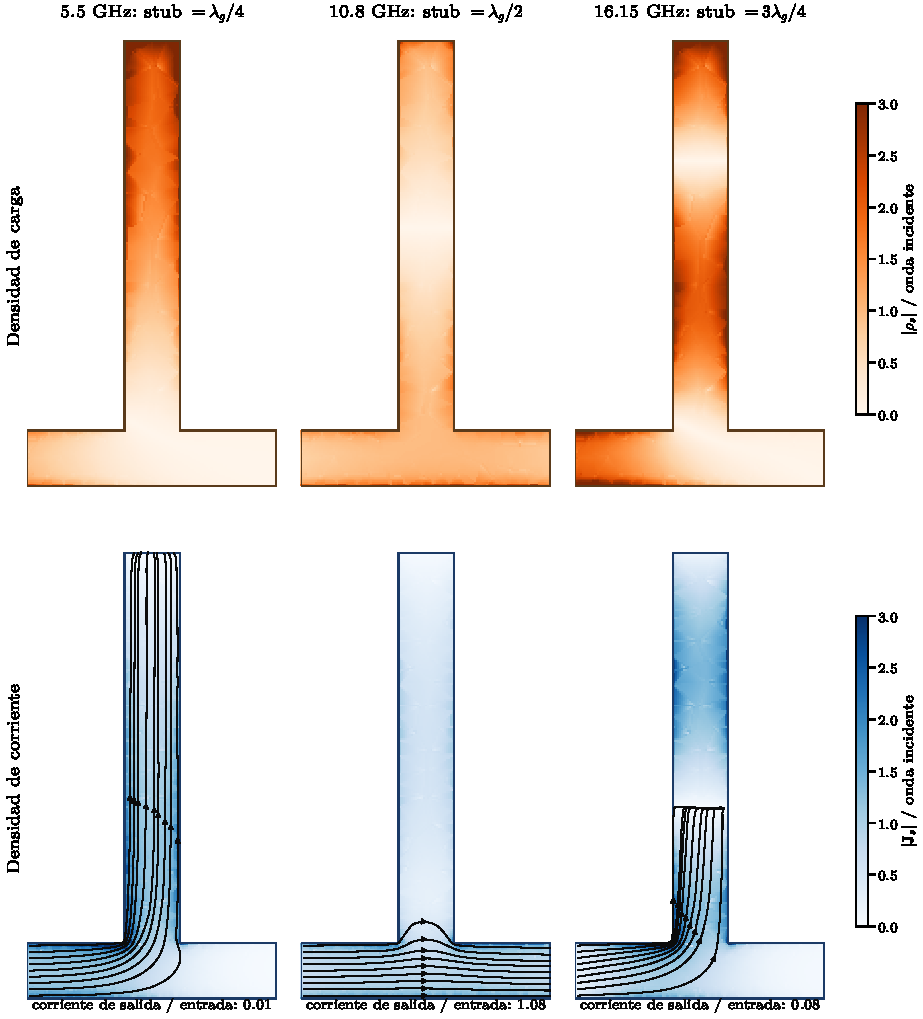
\includegraphics[width=0.94\textwidth]{figuras/fig_d5_stub_mapas.pdf}
\caption{Magnitud de la densidad superficial de carga (arriba) y de corriente (abajo) en el stub abierto, calculadas a partir de los campos de HFSS con la excitación por P1 (\SI{1}{W}), en las dos frecuencias de corte y en la de media onda. Ambas escalas están normalizadas a la onda incidente: el promedio en el brazo de entrada a \SI{10.8}{GHz}, donde la línea está acoplada. Las líneas de corriente parten del brazo de entrada y siguen la parte de $\mathbf{J}_s$ en fase con su corriente; a \SI{16.15}{GHz} se detienen en el nodo de corriente del stub, donde $\mathbf{J}_s$ cambia de sentido. Debajo de cada mapa, la corriente de la línea principal \SI{1.5}{mm} después de la unión dividida entre la de \SI{1.5}{mm} antes.}
\label{fig:d5stubmapas}
\end{figure}

La Figura~\ref{fig:d5stubonda} sigue la onda a lo largo del eje del stub. El voltaje se obtuvo integrando $E_z$ entre la tierra y la tira, y la corriente con la ecuación del telegrafista a partir de la derivada del voltaje. Los dos coinciden con la onda estacionaria de una línea abierta de longitud efectiva $\ell_{\mathrm{ef}}=\SI{<<D5S_LEF>>}{mm}$ (líneas discontinuas): voltaje máximo y corriente nula en el extremo, y nodos de voltaje cada $\lambda_g/2$ hacia la unión. A \SI{5.5}{GHz} el voltaje en el extremo abierto es <<D5S_VENDA>>\,$V_{\mathrm{inc}}$ y en la unión solo <<D5S_V0A>>\,$V_{\mathrm{inc}}$; en los ocho instantes de la Figura~\ref{fig:d5stubonda}c todo el stub oscila menos ese punto.

Al descomponer el voltaje medido en las dos ondas del stub, $V(s)=A\,e^{-\gamma s}+B\,e^{\gamma s}$ (error relativo del ajuste: <<D5S_ERRA>>\,\%), se ve por qué. La onda que sale de la unión hacia el extremo y la que regresa tienen casi la misma amplitud, $|A|=<<D5S_AA>>$ y $|B|=<<D5S_BA>>$ (en unidades de $V_{\mathrm{inc}}$), porque el extremo abierto refleja casi todo; y llegan a la unión desfasadas \ang{<<D5S_ANGA>>}, de modo que su suma es apenas <<D5S_SUMA>> veces $|A|$ (Figura~\ref{fig:d5stubonda}d). Un voltaje nulo en el punto donde se conecta el stub es un corto en paralelo con la línea principal. En un corto la onda incidente se refleja con $\Gamma=-1$ y la corriente se duplica; esa corriente no puede seguir hacia P2, que exigiría voltaje, y se va por el stub. Por eso la corriente en la base del stub es cercana a $2I_{\mathrm{inc}}$ y las ondas $A$ y $B$ son del orden de $V_{\mathrm{inc}}$.

\begin{figure}[htbp]
\centering
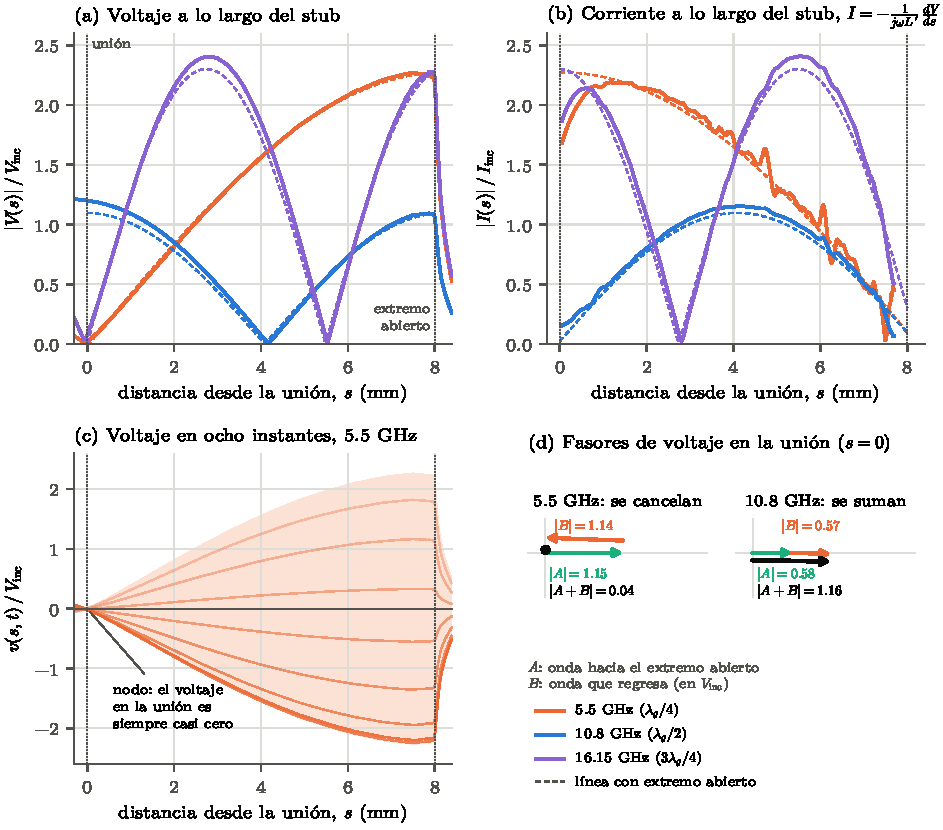
\includegraphics[width=\textwidth]{figuras/fig_d5_stub_onda.pdf}
\caption{Onda estacionaria en el stub, a partir de los campos de HFSS (excitación por P1, \SI{1}{W}). (a) Magnitud del voltaje entre la tira y la tierra a lo largo del eje del stub y (b) de la corriente, normalizados a los de la onda incidente; las líneas discontinuas son la onda estacionaria de una línea con extremo abierto, $|\cos\beta(\ell_{\mathrm{ef}}-s)|$ y $|\sin\beta(\ell_{\mathrm{ef}}-s)|$, con la amplitud medida en el extremo. (c) Voltaje instantáneo a \SI{5.5}{GHz} en ocho instantes de medio periodo; la banda es la envolvente $\pm|V(s)|$. (d) Las dos ondas del stub en la unión, $A$ (hacia el extremo abierto) y $B$ (la que regresa), obtenidas al ajustar $V(s)=A\,e^{-\gamma s}+B\,e^{\gamma s}$ al voltaje medido; las flechas se suman cabeza con cola.}
\label{fig:d5stubonda}
\end{figure}

A \SI{10.8}{GHz} las mismas dos ondas llegan a la unión casi en fase (\ang{<<D5S_ANGB>>} de diferencia) y se suman, $|A+B|=<<D5S_SUMB>>\,|A|$. El voltaje en la unión es máximo, la corriente en la base del stub es solo <<D5S_I0B>>\,$I_{\mathrm{inc}}$ y el nodo de voltaje queda a la mitad del stub (\SI{<<D5S_SMINB>>}{mm}): visto desde la línea, el stub es un circuito abierto, y la línea transmite como si no existiera. A \SI{16.15}{GHz} la onda que regresa ha recorrido $3\lambda_g/2$ y vuelve a llegar invertida (\ang{<<D5S_ANGC>>}). Hay otra vez un nodo de voltaje en la unión (<<D5S_V0C>>\,$V_{\mathrm{inc}}$), un segundo nodo a \SI{<<D5S_SMINC>>}{mm}, media longitud de onda más adelante ($\lambda_g/2=\SI{<<D5S_LG2C>>}{mm}$), y entre ambos el nodo de corriente donde se detienen las líneas de la Figura~\ref{fig:d5stubmapas}.

La radiación aparece en las resonancias, cuando el stub tiene una onda estacionaria grande (en el extremo abierto el voltaje pasa de dos veces el incidente) y su extremo abierto actúa como el borde de una antena de parche, igual que el gap de la discontinuidad 3. Que la predicción \eqref{eq:stubpred} funcione con un error de 1 a 2\,\% muestra que la unión, la línea y el extremo abierto se pueden tratar como bloques independientes y combinar: cada uno queda descrito por sus parámetros $S$, y lo que pasa en uno no depende de los demás.

\subsubsection{A partir de qué frecuencia el efecto es significativo}
Con el criterio de las otras discontinuidades ($|S_{11}|>-20$~dB), la T de \SI{50}{\ohm} es significativa en toda la banda y desde DC, porque su reflexión de un tercio la fija la división de impedancias. Lo que depende de la frecuencia es el reparto: el desbalance entre los dos brazos pasa de \SI{0.5}{dB} a partir de \SI{<<D5_FDESB05>>}{GHz}. En el divisor, donde la división de impedancias ya está resuelta, el efecto de la unión es significativo a partir de \SI{<<D5_FD20>>}{GHz}. Y el stub abierto es significativo a partir de \SI{<<D5_FS20>>}{GHz} (su capacitancia predice \SI{<<D5_FS20T>>}{GHz}), pero su efecto principal es una banda de corte cuya frecuencia fija la longitud de la rama, $f=c/\left(4\ell_{\mathrm{ef}}\sqrt{\varepsilon_{\mathrm{eff}}}\right)$: una derivación sin terminar de unos pocos milímetros corta la transmisión en la banda de los gigahertz.

%======================================================================
\section{Comparación entre discontinuidades}
\label{sec:comparacion}
La Tabla~\ref{tab:comparacion} resume las respuestas a la pregunta de investigación. Las cinco discontinuidades producen la reflexión por mecanismos distintos, y por eso dependen de la frecuencia de forma distinta. En la curva la línea es la misma de ambos lados y la reflexión la producen solo los parásitos, que crecen con $\omega$. En el cambio de ancho la reflexión la fija el cociente de impedancias y no depende de $\omega$. En el gap la conducción se interrumpe: la reflexión es casi total desde DC, y lo que crece con $\omega$ es la transmisión, a través del acoplamiento capacitivo. El cambio de sustrato es el caso más simple de todos: como la tira no cambia de forma, solo cambia $C'$ y la unión es un escalón de impedancia casi sin parásitos; la frecuencia interviene solo a través de la longitud eléctrica del tramo del otro material. El cambio de metal casi no refleja, y su efecto es una pérdida distribuida que crece como $\sqrt{f}$. La unión en T combina los dos tipos de mecanismo: una división de impedancias que refleja un tercio desde DC, como el cambio de ancho, y parásitos que crecen con $\omega$, como la curva, y que en este caso desequilibran el reparto de potencia.

Visto en conjunto, hay dos familias. En el cambio de ancho, el cambio de sustrato y la T, la reflexión principal es una diferencia de impedancias y está presente desde DC; la frecuencia solo importa a través de los parásitos o de la longitud eléctrica de un tramo. En la curva y en el divisor ya acoplado, la reflexión es solo parásita y aparece a partir de cierta frecuencia (\SI{<<F20>>}{GHz} y \SI{<<D5_FD20>>}{GHz}). El gap y el stub abierto son casos extremos. En el gap, el acoplamiento capacitivo es todo lo que une a las dos líneas, y la reflexión es casi total desde DC. En el stub, la rama abierta pone un corto en la línea en las frecuencias en que mide un número impar de cuartos de onda.

\begin{sidewaystable}
\centering
\caption{Comparación entre las discontinuidades estudiadas.}
\label{tab:comparacion}
\footnotesize
\renewcommand{\arraystretch}{1.25}
\setlength{\tabcolsep}{3.5pt}
\newcolumntype{P}[1]{>{\raggedright\arraybackslash}p{#1}}
\begin{tabular}{P{2.1cm}P{3.7cm}P{3.7cm}P{3.7cm}P{3.7cm}P{4.2cm}}
\toprule
 & Curva de \ang{90} & Cambio abrupto de ancho & Gap en serie & Cambio de material & Unión en T \\
\midrule
Origen de la reflexión & Desequilibrio de energías almacenadas en la esquina (parásitos) & Diferencia de impedancias características entre las líneas & Interrupción del camino de conducción & Sustrato: cambia solo $C'$, y con ella $Z_0$. Metal: casi ninguna & Cada brazo ve los otros dos en paralelo ($Z_0/2$); además, el cuadro de unión y el giro de la corriente \\
Dependencia con $f$ & $|\Gamma|\propto\omega$, nula en DC & $|\Gamma|\approx\Gamma_0$ constante desde DC & $|\Gamma|\approx 1$ desde DC; $|S_{21}|\propto\omega$ & $|\Gamma|\approx\Gamma_0$ constante desde DC; en un tramo, según $\ell/\lambda_g$ & $|\Gamma|\approx 1/3$ desde DC; el reparto se desequilibra con $\omega$ \\
$|S_{11}|>-20$~dB & A partir de \SI{<<F20>>}{GHz} & En toda la banda & En toda la banda & RO3010: en toda la banda (tramo: desde $\ell\approx\lambda_g/<<D4_LGF6>>$); FR-4 y estaño: nunca & T: en toda la banda; divisor: desde \SI{<<D5_FD20>>}{GHz}; stub: desde \SI{<<D5_FS20>>}{GHz} \\
Elementos parásitos & Capacitivos, dominan la respuesta & Capacitivos desde \SI{50}{\ohm}, casi nulos desde \SI{100}{\ohm}; solo giran la fase & $C_g$ (serie) fija la transmisión; $C_p$ (a tierra) alarga el extremo & No apreciables hasta \SI{10}{GHz}: los modos de ambos lados casi coinciden & $C_{\mathrm{ex}}\approx\SI{<<D5_CE_B_T>>}{fF}$ en el nodo e inductancia del giro hacia la rama; desbalance de \SI{<<D5_DESB20>>}{dB} a \SI{20}{GHz} \\
$|\Gamma|$ a \SI{20}{GHz} & <<GB20>> (VSWR <<VSWR20B>>) & <<D2_GB20>> (VSWR <<D2_VB20>>) & $\geq <<D3_G1_20>>$ (VSWR $\geq <<D3_VSWRG1_20>>$) & RO3010: <<D4_GB2_20>> (VSWR <<D4_VB2_20>>); FR-4: <<D4_GB1_20>>; estaño: $<<<D4_GDMAX_HI>>$ & Desde P1: <<D5_B11_20>>; desde la rama: <<D5_B33_20>> (VSWR <<D5_VB3_20>>) \\
Radiación a \SI{20}{GHz} & \SI{<<RADB20>>}{\percent}, por el giro de la corriente & $<\SI{<<D2_PRADCMAX>>}{\percent}$, la corriente no gira & \SIrange{<<D3_PRAD20MIN>>}{<<D3_PRAD20MAX>>}{\percent}, por el extremo abierto & $<\SI{<<D4_BALMAX4>>}{\percent}$, la corriente no gira & \SIrange{<<D5_PRADB1_20>>}{<<D5_PRADB3_20>>}{\percent}; stub: hasta \SI{<<D5_PRADD_MAX>>}{\percent} en resonancia \\
Corrección o variante & Chaflán: elimina la reflexión en toda la banda, no la radiación & Transición gradual: elimina la reflexión solo si $L_t\gtrsim<<D2_LTLGU>>\,\lambda_g$ & Gap más angosto: más $C_g$, pero solo transmite el 10\,\% desde \SI{<<D3_F10DB>>}{GHz} & Ajustar el ancho a \SI{50}{\ohm}: $|\Gamma|\leq <<D4_GCMAX>>$, pero la onda sigue más lenta & Divisor con salidas de \SI{100}{\ohm}: entrada acoplada hasta \SI{<<D5_FD20>>}{GHz}; rama abierta: corte en $\lambda_g/4$ (\SI{<<D5_FN1>>}{GHz}) \\
\bottomrule
\end{tabular}
\end{sidewaystable}

\section{Limitaciones}
\begin{itemize}
\item El piso numérico de los puertos limita la reflexión más pequeña que se puede resolver: alrededor de $-30$~dB sin corregir. En la curva con chaflán solo puede afirmarse que $|S_{11}|<\SI{-30}{dB}$. En el cambio de ancho la corrección con las referencias lo reduce, y la asimetría residual entre $|S_{11}|$ y $|S_{22}|$ (<<D2_ASIMB0_COR>>) indica su exactitud.
\item La radiación se obtiene por diferencia entre simulaciones y tiene una incertidumbre de $\pm\SI{<<PISO>>}{\percent}$ en la curva y $\pm\SI{<<D2_PISO2>>}{\percent}$ en el cambio de ancho.
\item La impedancia de una línea que no es TEM pura depende de su definición; en el cambio de ancho esto se manifiesta como una diferencia de \SI{<<D2_KPCT>>}{\percent} en el cociente $Z_2/Z_1$, absorbida por el parámetro $k$ del ajuste. Los datos fijan $C$ y $L_s$, pero no el reparto de $L_s$ entre ambos lados. En el cambio de sustrato, el escalón ideal se calculó con la impedancia $Z_{pi}$ de los puertos, y parte de la diferencia de hasta <<D4_DEVB2_20>> por encima de \SI{10}{GHz} puede deberse a la misma ambigüedad.
\item Los conductores se modelaron con espesor cero y sin rugosidad superficial, por lo que la potencia disipada es una estimación aproximada.
\item En el gap, la reflexión casi total amplifica el error de $|S_{11}|$ en el balance de potencia, por lo que la radiación tiene una incertidumbre de $\pm\SI{<<D3_PISO3>>}{\percent}$; además, cinco de sus diseños llegaron al máximo de pases con un solo pase bajo el criterio. El reparto de líneas de campo se calculó en un solo corte vertical y es una medida cualitativa.
\item En el cambio de material, la reflexión de la unión cobre--estaño queda por debajo de la resolución de la corrección (\SI{<<D4_RESREF4DB>>}{dB}); solo puede afirmarse que es menor, y la comparación con \eqref{eq:gsn} es indirecta, a través de las atenuaciones de HFSS. El tramo finito de la Figura~\ref{fig:d4tramo} se calculó combinando parámetros $S$, lo que supone que los campos evanescentes de una unión no alcanzan a la otra; es válido para tramos de varios $h$ de largo.
\item El estaño se modeló como un conductor macizo de conductividad finita. Un acabado real es una capa de pocos micrómetros sobre el cobre: cuando su espesor es menor que unas cuantas profundidades de penetración (\SI{<<D4_DSN01>>}{\micro\metre} a \SI{0.1}{GHz}, \SI{<<D4_DSN1>>}{\micro\metre} a \SI{1}{GHz} y \SI{<<D4_DSN20>>}{\micro\metre} a \SI{20}{GHz}), parte de la corriente circula por el cobre y la pérdida queda entre la del cobre y la calculada aquí. Tampoco se modeló la rugosidad ni el cambio de espesor de la pista estañada.
\item Los sustratos se tomaron con $\varepsilon_r$ y $\tan\delta$ constantes con la frecuencia, y con el mismo espesor; en una placa real con dos laminados también cambian el espesor y, en el FR-4, la permitividad con la frecuencia.
\item En la unión en T, el modelo de Hammerstad se evaluó con las impedancias y permitividades efectivas de los puertos de HFSS y no con las fórmulas cuasi-estáticas originales, y el divisor, con una rama de \SI{1.14}{mm} sobre una línea de \SI{0.29}{mm}, está probablemente fuera del rango para el que se ajustó el modelo. La capacitancia en exceso de la T de \SI{50}{\ohm} solo es constante entre 2 y \SI{5}{GHz}; por encima, el circuito de una sola capacitancia no basta. La predicción del stub usa el extremo abierto de otro proyecto (la discontinuidad 3), simulado con la misma configuración, y supone que los campos de la unión y del extremo no interactúan. Los campos se exportaron solo a \SI{5}{GHz} y con una sola excitación por estructura.
\item Se estudió un solo sustrato base, una sola relación de anchos en el cambio de ancho, cinco separaciones en el gap, tres materiales en el cambio de material y una sola geometría de cada variante de la T; los valores numéricos dependen de $h$, $\varepsilon_r$ y la geometría, aunque los mecanismos físicos son generales.
\end{itemize}

\section{Conclusiones}
\begin{resultado}
\textbf{Curva de \ang{90}.} La curva se comporta como una discontinuidad capacitiva: la esquina conserva la capacitancia de un tramo recto, pero la corriente la atraviesa por un camino más corto y su inductancia es menos de la mitad, por lo que equivale a un tramo corto de $\approx\SI{<<ZEQB>>}{\ohm}$ dentro de la línea de \SI{50}{\ohm}. Como la reactancia neta crece con $\omega$, la reflexión aumenta con la frecuencia y se vuelve significativa ($|S_{11}|>-20$~dB) a partir de \SI{<<F20>>}{GHz}, cuando la esquina mide apenas $\lambda_g/<<FRAC7>>$. A frecuencias mayores se suma la radiación, causada por el cambio de dirección de la corriente.
\end{resultado}

\begin{resultado}
\textbf{Cambio abrupto de ancho.} El empalme de una línea de \SI{50}{\ohm} con una de \SI{100}{\ohm} refleja $|\Gamma|\approx<<D2_GB01>>$ (VSWR $\approx<<D2_VB01>>$, el <<D2_PREFB>>\,\% de la potencia) desde las frecuencias más bajas, porque cada línea impone un cociente $V/I$ distinto. Su efecto es significativo en toda la banda y no depende de la frecuencia. Los parásitos de la unión, $C\approx\SI{<<D2_CEXC>>}{fF}$ por la carga de borde en los hombros y $L_s\approx\SI{<<D2_LEXC>>}{pH}$ por la concentración de la corriente, equivalen a unas decenas de micrómetros de línea y solo giran la fase de la reflexión (\ang{<<D2_ANGB20ABS>>} a \SI{20}{GHz}). El escalón no radia de forma apreciable porque la corriente no cambia de dirección.
\end{resultado}

\begin{resultado}
\textbf{Gap en serie.} Un corte en la tira interrumpe la conducción: en el extremo la corriente se anula, se forma una onda estacionaria y la potencia se refleja casi por completo desde DC ($|\Gamma|\geq <<D3_GMIN3>>$ en toda la banda). Lo único que cruza el corte es la corriente de desplazamiento a través de la capacitancia entre los extremos, $C_g$, que va de \SI{<<D3_CG0P1>>}{fF} con $s=\SI{0.1}{mm}$ a menos de \SI{1}{fF} con $s=\SI{3}{mm}$; por eso la transmisión crece 20~dB por década y solo el gap más angosto transmite más del 10\,\% de la potencia, a partir de \SI{<<D3_F10DB>>}{GHz}. El resto del campo del extremo baja a tierra ($C_p$, que tiende a la capacitancia de un extremo abierto). Los extremos abiertos radian, del orden de 3 a 5\,\% a \SI{20}{GHz}.
\end{resultado}

\begin{resultado}
\textbf{Cambio de material.} Si la tira continúa sobre otro sustrato, el campo magnético y la inductancia por unidad de longitud no cambian, pero el nuevo dieléctrico necesita más carga para sostener el mismo voltaje: $C'$ sube un factor de <<D4_RCP13>> al pasar a RO3010, $Z_0$ baja a \SI{<<D4_Z3_5>>}{\ohm} y la unión refleja $|\Gamma|\approx<<D4_GB2_5>>$ (VSWR $\approx<<D4_VB2_5>>$) desde DC, como predice $\Gamma_0=(n_1-n_2)/(n_1+n_2)$. Como la tira no cambia de forma, los modos de ambos lados casi coinciden y la unión no tiene parásitos apreciables por debajo de \SI{10}{GHz}; tampoco radia. Si el segundo sustrato ocupa un tramo, el efecto depende de su longitud eléctrica y es significativo cuando el tramo mide más de $\lambda_g/<<D4_LGF6>>$ (desde \SI{<<D4_FS6>>}{GHz} para \SI{6}{mm} de RO3010). El paso a FR-4 casi no refleja ($|\Gamma|\approx<<D4_GB1_5>>$), pero su línea atenúa <<D4_RFR5>> veces más. Cambiar el cobre por estaño no refleja de forma medible; su efecto es distribuido, una atenuación <<D4_DA5PCT>>\,\% mayor a \SI{5}{GHz} que crece como $\sqrt{f}$.
\end{resultado}

\begin{resultado}
\textbf{Unión en T.} En la unión las tres líneas comparten el voltaje y la corriente se reparte, de modo que cada brazo ve los otros dos en paralelo: con tres líneas de \SI{50}{\ohm}, la T refleja un tercio de la onda (VSWR $=<<D5_VB1_01>>$, el <<D5_PR11_01>>\,\% de la potencia) desde DC y entrega el <<D5_PT21_01>>\,\% a cada brazo. Ese efecto es significativo en toda la banda y no depende de la frecuencia. Lo que sí depende de ella es el reparto: el cuadro de unión se comporta como una capacitancia en el nodo de unos \SI{<<D5_CE_B_T>>}{fF}, y la corriente que entra a la rama tiene que doblar \ang{90}, lo que agrega inductancia a ese camino. A partir de \SI{<<D5_FDESB05>>}{GHz} el desbalance supera \SI{0.5}{dB}, y a \SI{20}{GHz} el <<D5_PT21_20>>\,\% de la potencia sigue de frente y solo el <<D5_PT31_20>>\,\% entra a la rama. El modelo de Hammerstad reproduce las fases, pero subestima esa energía almacenada. Con salidas de \SI{100}{\ohm} la entrada queda acoplada, y la reflexión que queda, la de la capacitancia de la unión (\SI{<<D5_CE_C_Divisor>>}{fF}), supera $-20$~dB a partir de \SI{<<D5_FD20>>}{GHz}. Una rama sin terminar de \SI{8}{mm} corta la transmisión a \SI{<<D5_FN1>>}{GHz} y \SI{<<D5_FN2>>}{GHz}, donde mide $\lambda_g/4$ y $3\lambda_g/4$.
\end{resultado}

\begin{itemize}
\item La curva sin compensar reduce la transmisión principalmente por reflexión: a \SI{20}{GHz} refleja el <<REFLB20>>\,\% de la potencia (VSWR $=<<VSWR20B>>$) y radia el <<RADB20>>\,\%. El chaflán óptimo ($M=55\,\%$) restituye $Z_{eq}\approx\SI{<<ZEQC>>}{\ohm}$ y elimina la reflexión en toda la banda, pero no la radiación.
\item Una transición gradual de \SI{10}{mm} entre las mismas líneas elimina la reflexión por encima de \SI{<<D2_FT20>>}{GHz}, cuando mide más de $<<D2_LTLGU>>\,\lambda_g$, y sigue la teoría de la transición exponencial sin parámetros ajustados; a baja frecuencia refleja igual que el escalón. Que un cambio sea ``abrupto'' depende de su longitud frente a $\lambda_g$, no de su forma.
\item En el gap, el tamaño del corte decide hacia dónde van las líneas de campo del extremo: al otro extremo ($C_g$) o a tierra ($C_p$). La suma de ambas capacitancias es casi constante, y el gap se comporta prácticamente como dos extremos abiertos cuando $s$ se acerca al ancho de la tira ($s/W\approx 1$).
\item En el cambio de sustrato, ajustar el ancho de la tira para conservar \SI{50}{\ohm} reduce la reflexión <<D4_RED>> veces a \SI{5}{GHz}: lo que refleja es la diferencia de impedancias y no la frontera entre materiales. La compensación no corrige la velocidad de propagación, que sigue siendo menor en el sustrato de mayor permitividad.
\item El stub abierto se predice con un error de \SI{<<D5_EFP1>>}{\percent} en la frecuencia de corte combinando los parámetros $S$ de la T, de la línea y del extremo abierto del gap, simulados por separado: cada discontinuidad es un bloque que se puede reutilizar en el análisis de un interconector completo.
\item No basta con observar que $S_{11}$ cambia: la extracción del circuito equivalente, la separación de la potencia en reflejada, radiada y disipada, y los campos de HFSS permiten identificar el mecanismo físico de cada efecto.
\item Las simulaciones de referencia con la misma configuración fueron indispensables, tanto para validar el montaje como para eliminar el error numérico común: en la curva para estimar la radiación, y en las demás discontinuidades además para corregir los parámetros $S$ completos. En el cambio de material hizo falta una referencia por cada tipo de línea, y sus constantes de propagación permitieron además separar las pérdidas del conductor y del dieléctrico.
\end{itemize}

\begin{thebibliography}{9}
\bibitem{pozar} D.~M. Pozar, \emph{Microwave Engineering}, 4th~ed. Hoboken, NJ, USA: Wiley, 2012.
\bibitem{gupta} K.~C. Gupta, R.~Garg, I.~Bahl y P.~Bhartia, \emph{Microstrip Lines and Slotlines}, 2nd~ed. Boston, MA, USA: Artech House, 1996.
\bibitem{douville} R.~J.~P. Douville y D.~S. James, ``Experimental study of symmetric microstrip bends and their compensation,'' \emph{IEEE Trans. Microw. Theory Techn.}, vol.~26, no.~3, pp.~175--182, 1978.
\bibitem{lewin} L.~Lewin, ``Radiation from discontinuities in strip-line,'' \emph{Proc. IEE, Part C}, vol.~107, no.~12, pp.~163--170, 1960.
\bibitem{rogers} Rogers Corporation, \emph{RO4000\textsuperscript{\textregistered} Series High Frequency Circuit Materials}, hoja de datos.
\bibitem{rogers3000} Rogers Corporation, \emph{RO3000\textsuperscript{\textregistered} Series Circuit Materials}, hoja de datos.
\bibitem{hammerstad} E.~Hammerstad, ``Computer-aided design of microstrip couplers with accurate discontinuity models,'' en \emph{IEEE MTT-S Int. Microwave Symp. Digest}, 1981, pp.~54--56.
\bibitem{qucs} S.~Jahn et al., \emph{Qucs Technical Papers}, sección ``Microstrip tee junction''. [En línea]. Disponible: \url{https://qucs.sourceforge.net/tech/node81.html}
\end{thebibliography}

\appendix
\section{Herramientas y métodos de cálculo}
\label{ap:metodos}

\subsection{Herramientas}
\begin{itemize}
\item \textbf{Ansys Electronics Desktop Student 2025~R2 (HFSS).} Solución de onda completa por elementos finitos en modo \emph{Driven Modal}. Los modelos no se dibujaron a mano: se construyeron, resolvieron y exportaron con scripts de la interfaz de automatización de AEDT escritos en Python. Para la curva: \texttt{P2\_D1\_Curva90\_v2.py} (seis estructuras), \texttt{P2\_Diagnostico\_Referencia.py} (variantes de la Tabla~\ref{tab:diag}) y \texttt{P2\_D1\_Exportar\_Campos.py} (campos de la Figura~\ref{fig:carga}). Para el cambio de ancho: \texttt{P2\_D2\_Escalon.py}, que construye las ocho estructuras, las resuelve, exporta los CSV y los campos y comprime los resultados; \texttt{P2\_D2\_Complemento.py} es el mismo script en modo complemento, que se usó para resolver con el límite de pases la transición sin pérdidas y agregar las referencias con pérdidas. Para el gap: \texttt{P2\_D3\_Gap.py}, que construye los doce diseños, los resuelve (y vuelve a resolver con menos pases cualquiera que exceda el límite de malla), exporta los CSV y los campos, incluido el corte vertical, y comprime los resultados. Para el cambio de material: \texttt{P2\_D4\_Material.py}, que construye los <<D4_NDIS4>> diseños con sus materiales (incluidos el FR-4, el RO3010 y la conductividad del estaño), los resuelve uno por uno, exporta los CSV y los campos y comprime los resultados; \texttt{P2\_D4\_Reanudar.py} es el mismo script en modo de reanudación, que abre el proyecto existente y resuelve solo los diseños que aún no tienen resultados. Para la unión en T: \texttt{P2\_D5\_T.py}, que construye los <<D5_NDIS5>> diseños (con tres puertos en la T y el divisor), los resuelve, exporta los CSV y los campos con la excitación indicada y comprime los resultados, \texttt{P2\_D5\_Reanudar.py}, su versión de reanudación, y \texttt{P2\_D5\_Campos\_Stub.py}, que agrega al stub tres puntos de frecuencia con campos guardados, los resuelve con la malla ya refinada y exporta los campos de las Figuras~\ref{fig:d5stubmapas} y~\ref{fig:d5stubonda}. Cada script crea las variables de diseño, la geometría, los materiales, las fronteras, los puertos, el análisis, las gráficas y la exportación de resultados.
\item \textbf{Python 3} con NumPy (aritmética compleja y álgebra lineal), SciPy (mínimos cuadrados no lineales, raíces e interpolación) y Matplotlib (figuras, exportadas como PDF vectorial). Con él se hizo todo el posprocesamiento y los cálculos auxiliares.
\item \textbf{\LaTeX} (pdflatex, con CircuiTikZ para los circuitos de las Figuras~\ref{fig:circescalon}, \ref{fig:circgap} y~\ref{fig:circt}). Las tablas y los valores numéricos citados en el texto se generan con un script directamente a partir de los datos de HFSS, sin transcripción manual.
\end{itemize}

El flujo de datos fue: HFSS $\rightarrow$ CSV y archivos de campo (parámetros $S$, impedancias y constantes de propagación de los puertos, balance de potencia, convergencia y campos $\mathbf{E}$ y $\mathbf{H}$) $\rightarrow$ Python (lectura, corrección, cálculo, figuras y tablas) $\rightarrow$ este documento. El código fuente se entrega junto con el reporte.

\subsection{Origen y método de cada figura y tabla}
\begin{description}[style=nextline,leftmargin=0pt,itemsep=4pt,font=\normalfont\bfseries]
\item[Sección~\ref{sec:diseno} (diseño de las líneas)] Evaluación numérica de \eqref{eq:eeff}, \eqref{eq:z0}, \eqref{eq:lg}, \eqref{eq:miter}, \eqref{eq:sintesis} y \eqref{eq:sintesis100}.

\item[Figuras~\ref{fig:geo}, \ref{fig:dgeo}, \ref{fig:d3geo}, \ref{fig:d4geo} y~\ref{fig:d5geo} (geometría)] Polígonos dibujados con Matplotlib a partir de las mismas dimensiones de los modelos de HFSS; el perfil de la transición se calcula con la misma rutina que usa el script de HFSS.

\item[Figuras~\ref{fig:hfss3d}, \ref{fig:dhfss}, \ref{fig:d3hfss}, \ref{fig:d4hfss} y~\ref{fig:d5hfss} (modelos 3D)] Capturas del modelador 3D de HFSS.

\item[Figuras~\ref{fig:circescalon}, \ref{fig:circgap} y~\ref{fig:circt} (circuitos)] Dibujadas con CircuiTikZ.

\item[Tabla~\ref{tab:conv} (convergencia)] Exportación de la convergencia del análisis adaptativo de HFSS: número de tetraedros y $\max|\Delta S|$ del último pase.

\item[Tabla~\ref{tab:diag} (diagnóstico)] Balance \eqref{eq:balance} evaluado a \SI{10}{GHz} con los CSV de las variantes de la línea de referencia.

\item[Figuras~\ref{fig:s11}, \ref{fig:gamma} y \ref{fig:s21}; Tabla~\ref{tab:sparam}] $|S_{11}|$ y $|S_{21}|$ en dB del barrido interpolante de HFSS (399 puntos entre \SI{0.1}{} y \SI{20}{GHz}); $|\Gamma|=10^{S_{11}[\mathrm{dB}]/20}$ y VSWR por \eqref{eq:merito}.

\item[Figura~\ref{fig:smith} (carta de Smith)] $S_{11}$ complejo exportado de HFSS. La retícula se trazó con la transformación bilineal $\Gamma=(z-1)/(z+1)$ aplicada a las curvas de resistencia y reactancia normalizadas constantes.

\item[Figura~\ref{fig:lc} y Tabla~\ref{tab:lc} (circuito de la curva)] Para cada punto de frecuencia se reconstruyó $S_{21}$ complejo a partir de su magnitud y fase, se convirtió la matriz $S$ a parámetros $Z$ con \eqref{eq:zparam} y se calcularon $C$, $L$ y $Z_{eq}$ con \eqref{eq:LC}. La tabla promedia de 3 a \SI{12}{GHz}; $\tau$ se obtiene de \eqref{eq:gamma_tau}.

\item[Figura~\ref{fig:rad} y Tabla~\ref{tab:potencia} (potencia en la curva)] Balance \eqref{eq:balance} para cada estructura y su gemelo sin pérdidas, y separación \eqref{eq:separacion}. La incertidumbre es el máximo de $|P_{\mathrm{rad}}|$ por debajo de \SI{6}{GHz}, donde la radiación debe ser nula.

\item[Figuras~\ref{fig:carga}, \ref{fig:dcarga} y~\ref{fig:d3campos} (carga y corriente)] Campos $\mathbf{E}$ y $\mathbf{H}$ exportados de HFSS en un punto de frecuencia de \SI{5}{GHz} con campos guardados, en una malla regular (paso de \SI{0.03}{mm} en la curva y la transición, \SI{0.02}{mm} en el escalón y el gap) sobre los planos $z=h\pm\SI{0.02}{mm}$. Cada campo se exportó en fase \ang{0} y \ang{90} para reconstruir el fasor, $\mathbf{F}=\mathbf{F}(\ang{0})-j\,\mathbf{F}(\ang{90})$. Con \eqref{eq:saltos} se obtuvieron $\rho_s$ y $\mathbf{J}_s$ en los puntos que caen sobre la traza. En la curva, las líneas de flujo se trazan con la parte real de $\mathbf{J}_s$ en la fase de máxima corriente del brazo; en el cambio de ancho, con la parte de $\mathbf{J}_s$ en fase con la corriente total de cada sección, lo que quita el retardo de la onda a lo largo de la línea. Los repartos de la curva son la suma de $|\rho_s|$ en cada mitad del cuadrado de la esquina, separadas por la diagonal $x=y$, y la integral de $\mathbf{J}_s\cdot\hat{\mathbf{n}}$ a lo largo de la diagonal que une la esquina interior con la exterior, con interpolación bilineal. En el cambio de ancho, $q(x)$ es la suma de $\rho_s$ a lo ancho de la traza en cada sección; el escalón ideal es la recta ajustada a $q(x)$ en cada línea, lejos del escalón, extrapolada hasta el plano de unión; y la fracción de corriente es la suma de $|J_x|$ en $|y|<W_2/2$ entre la suma en todo el ancho.

\item[Figuras~\ref{fig:escala} y~\ref{fig:descala} (escala de la onda)] $\lambda_g$ de \eqref{eq:lg} con $\varepsilon_{\mathrm{eff}}$ de \eqref{eq:eeff} (en la transición, el promedio de ambas líneas); onda $\cos(2\pi s/\lambda_g)$ y desfase $\Delta\phi=\ang{360}\,W\sqrt{2}/\lambda_g$. En la Figura~\ref{fig:descala}a el eje horizontal es $L_t/\lambda_g$ evaluado en cada frecuencia del barrido, y la teoría es \eqref{eq:taper}.

\item[Figura~\ref{fig:imagen} (tira e imagen)]
(a) Campo magnetostático bidimensional: la tira se representa con 41 corrientes filamentarias repartidas en su ancho y su imagen con las corrientes opuestas a una distancia $2h$; el campo es la superposición $\mathbf{B}\propto\sum_k I_k\,\hat{\mathbf{z}}\times(\mathbf{r}-\mathbf{r}_k)/|\mathbf{r}-\mathbf{r}_k|^2$. El color es $\log_{10}|\mathbf{B}|$ y las líneas son líneas de campo.
(b) $|\mathbf{B}|$ sobre el eje vertical de la tira para la tira sola y para el par tira--imagen.
(c) Esquema dibujado en proyección oblicua; es ilustrativo y no proviene de un cálculo.

\item[Tabla~\ref{tab:dlineas} (líneas del cambio de ancho)] Impedancia de los puertos (parte real de $Z_{pi}$) y $\varepsilon_{\mathrm{eff}}=(\mathrm{Im}\{\gamma\}/k_0)^2$ exportados de HFSS, promediados entre los dos puertos de cada referencia sin pérdidas.

\item[Figura~\ref{fig:dcorr} (corrección de puertos)] Ajuste lineal por mínimos cuadrados de los coeficientes del polinomio $g(f)$ en \eqref{eq:gpuerto}, con $\beta$ de cada puerto y el promedio de $S_{11}$ y $S_{22}$ de la referencia. Cada caja de error tiene $E_{11}=g\,e^{2j\beta L_1}$, $E_{22}=-g\,e^{-2j\beta L_1}$ y $E_{21}^2=S_{21}^{\mathrm{ref}}(1-E_{22}^2)$, de modo que dos cajas en espejo reproducen la referencia. La conversión entre parámetros $S$ y matrices de transferencia es $\mathbf{T}=\frac{1}{S_{21}}\begin{pmatrix}S_{12}S_{21}-S_{11}S_{22} & S_{11}\\ -S_{22} & 1\end{pmatrix}$, y \eqref{eq:deembed} se evalúa en cada frecuencia.

\item[Figuras~\ref{fig:dsdb}, \ref{fig:dgamma} y~\ref{fig:dsmith}; Tabla~\ref{tab:dsparam}] Parámetros $S$ complejos exportados de HFSS y corregidos con \eqref{eq:deembed}; $|\Gamma|$, VSWR y pérdidas por \eqref{eq:merito}. Las curvas teóricas son \eqref{eq:gamma0} con las impedancias de \eqref{eq:z0} y \eqref{eq:taper} con $\beta=k_0\sqrt{\varepsilon_{\mathrm{eff}}}$ promedio. Los cruces y nulos se buscan directamente en los 399 puntos del barrido.

\item[Figura~\ref{fig:dfase} y Tabla~\ref{tab:dfit} (circuito del escalón)] (a) Fase de $S_{11}$ y de $-S_{22}$ corregidos. (b) $\mathrm{Im}\{Z_{\mathrm{ent}}\}$ con $Z_{\mathrm{ent},1}=Z_1(1+S_{11})/(1-S_{11})$ y $Z_{\mathrm{ent},2}=Z_2(1+S_{22})/(1-S_{22})$, con $Z_1$ y $Z_2$ de los puertos. El ajuste minimiza, con \texttt{scipy.optimize.least\_squares}, la diferencia compleja entre los parámetros $S$ corregidos y los del circuito de la Figura~\ref{fig:circescalon}, calculados con su matriz $ABCD$ y las impedancias de referencia $Z_1$ y $kZ_2$. La incertidumbre es la mitad del intervalo entre los ajustes del diseño con y sin pérdidas en los rangos 1--20, 3--20 y 1--\SI{12}{GHz}. Las fórmulas de Gupta et al.\ son \eqref{eq:gupta}.

\item[Figura~\ref{fig:dpot} y Tabla~\ref{tab:dpot} (potencia en el cambio de ancho)] Balance \eqref{eq:balance} con los parámetros corregidos, promediando la excitación desde cada puerto: radiada $=P_{X0}$ del gemelo sin pérdidas corregido (la corrección ya quita el residuo de las referencias) y disipada $=P_X-P_{X0}$. La incertidumbre es el valor negativo más grande de la radiada, que físicamente no puede ser negativa. La pérdida esperada de la transición es $1-e^{-2\bar\alpha L_t}$, con $\bar\alpha$ el promedio de la parte real de la constante de propagación de ambos puertos.

\item[Tabla~\ref{tab:d3sparam} y Figura~\ref{fig:d3s} (gap: parámetros $S$)] Parámetros $S$ complejos corregidos con \eqref{eq:deembed}, usando la misma caja de error (línea de \SI{50}{\ohm}) en ambos puertos. La pendiente se calcula entre 1 y \SI{10}{GHz}; la curva del extremo abierto en (b) es $-2\arctan(\omega C_{oc}Z_0)$ con $C_{oc}$ de \eqref{eq:dloc}.

\item[Figura~\ref{fig:d3cap} y Tabla~\ref{tab:d3circ} (gap: circuito $\pi$)] En cada frecuencia, $\mathbf{Y}=\mathbf{Z}_r^{-1/2}(\mathbf{I}-\mathbf{S})(\mathbf{I}+\mathbf{S})^{-1}\mathbf{Z}_r^{-1/2}$, con $\mathbf{Z}_r$ la matriz diagonal de las impedancias de los puertos, y $C_g$, $C_p$ con \eqref{eq:ygap} ($C_p$ es el promedio de ambos extremos). Las fórmulas de Garg y Bahl son \eqref{eq:gargbahl}; la del extremo abierto, \eqref{eq:dloc} con $C'$ de la línea.

\item[Figura~\ref{fig:d3pot} y Tabla~\ref{tab:d3pot} (gap: potencia)] Balance \eqref{eq:balance} con los parámetros corregidos, promediando la excitación desde cada puerto; radiada $=P_{X0}$ y disipada $=P_X-P_{X0}$. La incertidumbre es $2\max|S_{11}|$ de la referencia corregida, que es el error que deja la corrección en $|S_{11}|^2$ cuando $|S_{11}|\approx 1$.

\item[Figura~\ref{fig:d3campos} (gap: carga y líneas de campo)] La carga se calcula como en las demás figuras de campos, y los cocientes de carga son la suma de $\rho_s$ en el último \SI{0.5}{mm} de cada tira. El corte vertical se exportó en el plano $y=0$ con paso de \SI{0.01}{mm}; por simetría, ahí $E_y=0$ y las líneas de campo quedan en el plano. Las líneas se integran con pasos de \SI{4}{\micro\metre} a lo largo de la dirección de $\mathrm{Re}\{\mathbf{E}\}$ en la fase en que la carga del extremo es máxima, partiendo de 60 puntos en cada cara de la tira; cada línea se pesa con $\varepsilon|E_z|$ en su punto de partida y se clasifica según toque la tira derecha, el plano de tierra o el borde del corte.

\item[Tabla~\ref{tab:d4lineas} (líneas del cambio de material)] De cada referencia: $Z_0=\mathrm{Re}\{Z_{pi}\}$ y $\gamma=\alpha+j\beta$ del puerto, $\varepsilon_{\mathrm{eff}}=(\beta/k_0)^2$, $n=\sqrt{\varepsilon_{\mathrm{eff}}}$, $L'=Z_0n/c$, $C'=n/(cZ_0)$ y $\alpha$ en dB/cm $=8.686\,\alpha/100$, a \SI{5}{GHz}. La columna \eqref{eq:z0} usa \eqref{eq:eeff} con la $\varepsilon_r$ de cada sustrato.

\item[Figura~\ref{fig:d4refl} y Tabla~\ref{tab:d4sparam} (cambio de material: reflexión)] Parámetros $S$ complejos corregidos con \eqref{eq:deembed}, con la caja de error de RO4003C en el puerto 1 y la de la referencia del segundo material en el puerto 2. El escalón ideal es \eqref{eq:gamma0} con $\mathrm{Re}\{Z_{pi}\}$ de los dos puertos de cada diseño en cada frecuencia, y \eqref{eq:gamman} con los índices de la Tabla~\ref{tab:d4lineas}. La resolución es el máximo de $|S_{11}|$ de las cinco referencias corregidas con sus propias cajas. La curva teórica del estaño es \eqref{eq:gsn} con $\Delta\alpha_c$ de la Figura~\ref{fig:d4perd} y $\beta$ del puerto de RO4003C.

\item[Figura~\ref{fig:d4perd} y Tabla~\ref{tab:d4alfa} (pérdidas)] $\alpha$ de los puertos de las referencias de cobre y de estaño sobre RO4003C; $\alpha_d$ de \eqref{eq:alfad} con $\varepsilon_{\mathrm{eff}}$ de HFSS, y $\alpha_c=\alpha-\alpha_d$. La fracción de la pérdida de conductor en la tira es $(r-1)/(\sqrt{\sigma_{\mathrm{Cu}}/\sigma_{\mathrm{Sn}}}-1)$, con $r=\alpha_{c,\mathrm{Sn}}/\alpha_{c,\mathrm{Cu}}$, promediada entre 1 y \SI{20}{GHz}, y el exponente de $f$ es la pendiente de $\ln\alpha_c$ contra $\ln f$ en ese rango. El balance de los gemelos sin pérdidas es \eqref{eq:balance} con los parámetros corregidos, promediando la excitación desde cada puerto.

\item[Ajuste del sustrato compensado] Mismo procedimiento que la Tabla~\ref{tab:dfit}, con $L_s$ repartida en proporción a $L'$ de cada línea ($\alpha=<<D4_ALFA4>>$) y la incertidumbre como la mitad del intervalo entre seis ajustes (con y sin pérdidas, en 1--20, 3--20 y 1--\SI{12}{GHz}).

\item[Figura~\ref{fig:d4tramo} y Tabla~\ref{tab:d4tramo} (tramo finito)] Cascada de matrices de transferencia $\mathbf{T}_J\,\mathbf{T}_\ell\,\mathbf{T}_{J'}$, donde $\mathbf{T}_J$ es la unión corregida, $\mathbf{T}_{J'}$ la misma unión vista desde el otro lado ($S_{11}\leftrightarrow S_{22}$) y $\mathbf{T}_\ell=\mathrm{diag}(e^{-\gamma\ell},e^{\gamma\ell})$ con $\gamma$ del puerto de la referencia del segundo material. El cruce de 0.1 se interpola linealmente entre los dos puntos del barrido que lo rodean, y la longitud eléctrica en el cruce es $\lambda_g/\ell$ con $\lambda_g=c/(f\sqrt{\varepsilon_{\mathrm{eff}}})$ en esa frecuencia.

\item[Figura~\ref{fig:d4campos} (campos del cambio de sustrato)] Campos exportados igual que en las otras discontinuidades (\SI{5}{GHz}, paso de \SI{0.02}{mm} en los planos $z=h\pm\SI{0.02}{mm}$ y de \SI{0.01}{mm} en el plano $y=0$). $\rho_s$ usa en cada punto la $\varepsilon_r$ del sustrato que tiene debajo, y se descarta la columna $x=L_1$, que cae sobre la frontera. $q(x)$ e $I(x)$ son las sumas de $\rho_s$ y $J_x$ a lo ancho de la tira; $V(x)$ es la integral de $E_z$ desde la tierra hasta la tira en $y=0$, con la regla del trapecio. Las tres se suavizan con una media móvil de \SI{0.1}{mm} sin mezclar los dos lados de la unión. Los saltos citados en el texto son cocientes de promedios a cada lado de la unión, lejos de ella para $q$ y $\mathbf{D}$ y a menos de \SI{0.3}{mm} para $V$, $I$ y $\mathbf{E}$.

\item[Tabla~\ref{tab:d5sparam} y Figura~\ref{fig:d5t} (T de \SI{50}{\ohm})] Parámetros $S$ de tres puertos leídos de HFSS (el orden de las columnas se toma del encabezado del CSV) y corregidos con \eqref{eq:deembedn}. La T ideal es \eqref{eq:tideal} con $\mathrm{Re}\{Z_{pi}\}$ de cada puerto. El desbalance es $20\log_{10}(|S_{21}|/|S_{31}|)$ y sus cruces se interpolan linealmente entre los puntos del barrido.

\item[Modelo de Hammerstad] Las ecuaciones \eqref{eq:hammerstad} se transcribieron del código fuente del simulador Qucs (\texttt{mstee.cpp}) y se evaluaron en cada frecuencia con la impedancia y la permitividad efectiva de los puertos de las referencias sin pérdidas. La red de la Figura~\ref{fig:circt} se resolvió con su matriz de impedancias: el nodo con $B_T$ y los transformadores dan $\mathbf{Z}_c=\mathbf{u}\mathbf{u}^T/(jB_T)$ con $\mathbf{u}=(1/T_a,1/T_b,1)$, y cada tramo de línea, con su matriz $ABCD$, da $\mathbf{Z}=(\mathbf{A}\mathbf{Z}_c+\mathbf{B})(\mathbf{C}\mathbf{Z}_c+\mathbf{D})^{-1}$; $\mathbf{S}$ se obtiene con las mismas impedancias de referencia que HFSS. Con todos los puertos a la misma impedancia, este cálculo coincide con las expresiones de Qucs.

\item[Figura~\ref{fig:d5div} y Tabla~\ref{tab:d5div} (divisor y capacitancia en exceso)] $Y_{\mathrm{ent},3}=(1-S_{33})/[(1+S_{33})Z_3]$ con los parámetros corregidos, y $C_{\mathrm{ex}}=[\mathrm{Im}\{Y_{\mathrm{ent},3}\}-\mathrm{Im}\{1/Z_1+1/Z_2\}]/\omega$. El valor citado es el promedio de los diseños con y sin pérdidas entre 2 y \SI{5}{GHz} (T) o 2 y \SI{15}{GHz} (divisor); la incertidumbre es la mayor entre su diferencia y la variación con la frecuencia. $C'W$ usa $C'=\sqrt{\varepsilon_{\mathrm{eff}}}/(cZ_0)$ de la referencia a \SI{5}{GHz}.

\item[Tabla~\ref{tab:d5pot} (potencia en la T)] Para la excitación desde el puerto $j$, la potencia que no sale por ningún puerto es $1-\sum_i|S_{ij}|^2$; radiada la del gemelo sin pérdidas y disipada la diferencia. La incertidumbre es el valor negativo más grande de la radiada por debajo de \SI{8}{GHz}.

\item[Figura~\ref{fig:d5stub} (stub)] Mínimos de $|S_{21}|$ buscados en los puntos del barrido. La predicción es \eqref{eq:stubpred} con los parámetros corregidos de la T, $\gamma$ del puerto de la referencia de \SI{50}{\ohm}, $\ell=\SI{8}{mm}$ y $\Gamma_{\mathrm{oc}}=S_{11}$ corregido del gap de \SI{3}{mm} de la discontinuidad 3 (o $e^{-2j\beta\Delta\ell}$ con \eqref{eq:dloc}). La extensión del extremo abierto es $-\angle\Gamma_{\mathrm{oc}}/(2\beta)$, promediada entre 2 y \SI{15}{GHz}. La radiación es el promedio de la excitación desde cada puerto del gemelo sin pérdidas corregido.

\item[Figura~\ref{fig:d5campos} (campos de la T)] Campos exportados a \SI{5}{GHz} en los planos $z=h\pm\SI{0.02}{mm}$ con paso de \SI{0.02}{mm}, después de fijar la excitación con \texttt{EditSources} (solo P1 en la T y solo P3 en el divisor, \SI{1}{W}). $\rho_s$ y $\mathbf{J}_s$ como en las demás figuras de campos. Las corrientes de cada brazo son la suma de $J_x$ o $J_y$ a lo ancho de la traza en una sección a \SI{1.2}{mm} del cuadro de unión; las líneas de flujo parten de 15 puntos a lo ancho del brazo de entrada y siguen la parte de $\mathbf{J}_s$ en fase con la corriente de entrada. Los factores son promedios de $|\rho_s|$ en el cuadro de unión y de $|\mathbf{J}_s|$ en cuadros de \SI{0.15}{mm} en las esquinas interiores, respecto al brazo de entrada.

\item[Figuras~\ref{fig:d5stubmapas} y~\ref{fig:d5stubonda} (campos del stub)] Puntos de frecuencia discretos a \SI{5.5}{}, \SI{10.8}{} y \SI{16.15}{GHz} agregados al diseño del stub y resueltos con la malla ya refinada, con la excitación solo por P1 (\SI{1}{W}, \texttt{EditSources}). $\rho_s$ y $\mathbf{J}_s$ en los planos $z=h\pm\SI{0.02}{mm}$ con paso de \SI{0.04}{mm}, como en las demás figuras de campos, normalizadas a sus promedios en el brazo de entrada ($x$ de \SI{4.1}{} a \SI{4.9}{mm}) a \SI{10.8}{GHz}. El cociente de corrientes bajo cada mapa es $|\sum J_x\,\Delta y|$ a lo ancho de la línea en $x=L_1+W+\SI{1.5}{mm}$ entre el mismo valor en $x=L_1-\SI{1.5}{mm}$; al ser un cociente en la misma malla, no le afecta la subestimación de la corriente total que causa la singularidad de $\mathbf{J}_s$ en los bordes de la tira. El voltaje es $V(s)=-\int_0^h E_z\,dz$ en un corte vertical por el eje del stub, con paso de \SI{0.02}{mm} y el fasor $E(\ang{0})-jE(\ang{90})$. La corriente sale de la ecuación del telegrafista, $I=-(1/j\omega L')\,dV/ds$, con $L'=Z_0\sqrt{\varepsilon_{\mathrm{eff}}}/c$ del puerto de la referencia de \SI{50}{\ohm} y la derivada calculada con un filtro de Savitzky--Golay (ventana de \SI{0.4}{mm}, polinomio cúbico); se usó en lugar de integrar $\mathbf{J}_s$ por la misma singularidad de borde. Ambos se normalizan a la onda incidente de \SI{1}{W}, $V_{\mathrm{inc}}=\sqrt{2PZ_0}$ e $I_{\mathrm{inc}}=V_{\mathrm{inc}}/Z_0$. Las curvas de línea abierta usan $\beta$ del puerto y $\ell_{\mathrm{ef}}=\ell+\Delta l$ con la $\Delta l$ medida en el gap de \SI{3}{mm}, y su amplitud es el voltaje medido cerca del extremo. $A$ y $B$ salen de un ajuste lineal por mínimos cuadrados de $A\,e^{-\gamma s}+B\,e^{\gamma s}$ entre $s=\SI{0.4}{}$ y \SI{7.4}{mm}, lejos de la unión y del extremo, con $\gamma$ del puerto.
\end{description}

\end{document}
